\documentclass[preprint, 12pt]{elsarticle}
%DIF LATEXDIFF DIFFERENCE FILE



% For journal layout:
% \documentclass[final,1p,times]{elsarticle}
% \documentclass[final,1p,times,twocolumn]{elsarticle}
% \documentclass[final,3p,times]{elsarticle}
% \documentclass[final,3p,times,twocolumn]{elsarticle}
% \documentclass[final,5p,times]{elsarticle}
% \documentclass[final,5p,times,twocolumn]{elsarticle}

%% Use packages ---------------------------------------------
\usepackage[english]{babel}
\usepackage{amssymb} 
\usepackage{amsmath}
\usepackage{amsfonts}
\usepackage{color}
\usepackage{subcaption}
%DIF 18a18-23
\usepackage{framed} % Framing content %DIF > 
\usepackage{nomencl} % Nomenclature package %DIF > 
\usepackage{booktabs} %DIF > 
\usepackage{siunitx} % SI units %DIF > 
\makenomenclature %DIF > 
\setlength{\nomitemsep}{-\parskip} % Baseline skip between items %DIF > 
%DIF -------

%% Customization --------------------------------------------
% New commands Tasora 
\def\vect#1{{\boldsymbol{#1}}}
\def\quat#1{{\boldsymbol{#1}}}
\def\conj{\hskip0.1em^*} % the matrix as [R(a)] , with letter between two (autoresizing) square brackets
\def\amatr#1{{#1}}
\newcommand{\norm}[1]{\left\lVert#1\right\rVert}

% New commands Fusai 
\newcommand{\hl}[1]{\textcolor{red}{#1}}

%% Document ----------------------------------------------
%DIF PREAMBLE EXTENSION ADDED BY LATEXDIFF
%DIF UNDERLINE PREAMBLE %DIF PREAMBLE
\RequirePackage[normalem]{ulem} %DIF PREAMBLE
\RequirePackage{color}\definecolor{RED}{rgb}{1,0,0}\definecolor{BLUE}{rgb}{0,0,1} %DIF PREAMBLE
\providecommand{\DIFadd}[1]{{\protect\color{blue}\uwave{#1}}} %DIF PREAMBLE
\providecommand{\DIFdel}[1]{{\protect\color{red}\sout{#1}}}                      %DIF PREAMBLE
%DIF SAFE PREAMBLE %DIF PREAMBLE
\providecommand{\DIFaddbegin}{} %DIF PREAMBLE
\providecommand{\DIFaddend}{} %DIF PREAMBLE
\providecommand{\DIFdelbegin}{} %DIF PREAMBLE
\providecommand{\DIFdelend}{} %DIF PREAMBLE
%DIF FLOATSAFE PREAMBLE %DIF PREAMBLE
\providecommand{\DIFaddFL}[1]{\DIFadd{#1}} %DIF PREAMBLE
\providecommand{\DIFdelFL}[1]{\DIFdel{#1}} %DIF PREAMBLE
\providecommand{\DIFaddbeginFL}{} %DIF PREAMBLE
\providecommand{\DIFaddendFL}{} %DIF PREAMBLE
\providecommand{\DIFdelbeginFL}{} %DIF PREAMBLE
\providecommand{\DIFdelendFL}{} %DIF PREAMBLE
%DIF END PREAMBLE EXTENSION ADDED BY LATEXDIFF

\begin{document}

\journal{Mechanism and Machine Theory}

\begin{frontmatter}

% Title
\title{A practical algorithm for smooth interpolation between different angular positions}

% Authors and affiliations
\author[1,2,*]{Giovanni Legnani}
\author[2]{Irene Fassi}
\author[3]{Alessandro Tasora}
\author[3]{Dario Fusai}
\address[*]{corresponding author, giovanni.legnani@unibs.it}
\address[1]{DIMI-UniBS Dipartimento Ingegneria Meccanica e Industriale, Università di Brescia, Via Branze 38, 25123 Brescia, Italy}
\address[2]{STIIMA-CNR Istituto di Sistemi e Tecnologie Industriali per il Manifatturiero Avanzato, National Research Council, Via Alfonso Corti 12, 20133 Milano, Italy}
\address[3]{Dipartimento di Ingegneria e Architettura, Università di Parma, Parco Area delle Scienze, 181/A - 43124 PARMA, Italy}

% Abstract
\begin{abstract}
This paper proposes a new methodology for the interpolation of a \DIFdelbegin \DIFdel{sequence }\DIFdelend \DIFaddbegin \DIFadd{given set }\DIFaddend of 3D \DIFdelbegin \DIFdel{orientation poses }\DIFdelend \DIFaddbegin \DIFadd{rotation poses that have }\DIFaddend to be reached in successive times by preserving continuity in orientation, angular velocity and angular acceleration. The \DIFdelbegin \DIFdel{methodology }\DIFdelend \DIFaddbegin \DIFadd{discussed algorithm }\DIFaddend ensures the generation of smooth angular trajectories without singularities. The distinctive features of the proposed approach are the straightforward formulation\DIFdelbegin \DIFdel{and }\DIFdelend \DIFaddbegin \DIFadd{, }\DIFaddend the reduced computational burden \DIFaddbegin \DIFadd{and the lack of iterative procedures}\DIFaddend . The presented methodology has applications in the generation of spatial motion of mechanical systems (e.g. robotics, flying devices) or in 3D computer graphics. After a theoretical introduction, the proposed algorithm is compared with other methods available in literature and some possible applications are presented.
\end{abstract}

% Keywords
\begin{keyword}
\DIFdelbegin \DIFdel{Rotations }\DIFdelend \DIFaddbegin \DIFadd{Smooth rotation interpolation }\DIFaddend \sep \DIFdelbegin \DIFdel{quaternions }\DIFdelend \DIFaddbegin \DIFadd{Angular trajectory }\DIFaddend \sep \DIFdelbegin \DIFdel{trajectories }\DIFdelend \DIFaddbegin \DIFadd{Rotations }\DIFaddend \sep \DIFdelbegin \DIFdel{robotics
}\DIFdelend \DIFaddbegin \DIFadd{Quaternions
}\DIFaddend \end{keyword}

\end{frontmatter}

% Sections
\section{Introduction}
\label{sec:introduction}
In many theoretical and application fields there is the need to interpolate between a \DIFdelbegin \DIFdel{set of different }\DIFdelend \DIFaddbegin \DIFadd{given set of }\DIFaddend configurations in 3D space\DIFaddbegin \DIFadd{, in order }\DIFaddend to obtain a smooth motion of a rigid frame. This \DIFaddbegin \DIFadd{is }\DIFaddend a typical problem of industrial robotics (for manipulation, welding, or inspection) \DIFaddbegin \DIFadd{ 
\cite{li2009research}  
 
\cite{neubauer2015smooth} 
}\DIFaddend , aerospace (for path planning) \DIFaddbegin \DIFadd{ 
\cite{yongguo2010trajectory}  
}\DIFaddend and computer graphics areas (for camera motions) \DIFaddbegin \DIFadd{ 
\cite{shoemake1985animating} 
}\DIFaddend , but it also has applications in the field of computational solid mechanics \DIFdelbegin \DIFdel{ 
\cite{bauchau2014interpolation} 
}\DIFdelend \DIFaddbegin \DIFadd{(see, for example,  
\cite{romero2004interpolation} 
,  
\cite{ghosh2008consistent}  
and  
\cite{bauchau2014interpolation} 
)}\DIFaddend . It is known that the motion of a rigid body in 3D space is representable by the combination of a translation and a rotation relative to a reference frame: motion interpolation is therefore the act of producing two continuous curves (one in $\mathbb{R}^{3}$ and the other in $\mathsf{SO}(3)$) from a set of \emph{key frames}. The problem of spatial interpolation in Euclidean $\mathbb{R}^{3}$ space has been thoroughly studied and many operative algorithms are available, spacing from simple linear interpolation to smooth B\'ezier, B-Spline and NURBS curves. On the other hand, the interpolation of orientations still poses some difficulties, due to the peculiar characteristics of rotations in 3D space.

As a matter of fact, the orientation of solid objects is mathematically representable in many ways: rotation matrices, axis-angle formalism, Rodrigues vectors and quaternions are only part of a numerous list of possibilities. Each of these representation \DIFdelbegin \DIFdel{offer }\DIFdelend \DIFaddbegin \DIFadd{offers }\DIFaddend both advantages and drawbacks, making them individually suitable for a specific application and less for another. For example, if we parametrize a rotation matrix through Cardan angles (both in the intrinsic Euler $Z-X^{'}-Z^{''}$ form or in the extrinsic Tait-Bryan $X-Y-Z$ one), we obtain a straightforward and intuitive method \DIFdelbegin \DIFdel{which }\DIFdelend \DIFaddbegin \DIFadd{that }\DIFaddend allows us to combine successive rotations with simple linear algebra operations (see \ref{app:RotatMatrix} for more information). However, a major problem of this approach is that any adopted set of angles will have at least one configuration leading to singularity, making such choice unfit for generic applications.
%DIF < : we thus lose the one-to-one correspondence between representation (matrix) and quantity represented (rotation). Moreover, even if the representation is based on three independant parameters, we constantly have to deal with nine numbers (3x3 matrix). 

A better strategy is to represent rotations by the means of unit quaternions \cite{hamilton1844ii}. These mathematical objects possess four \DIFdelbegin \DIFdel{independent }\DIFdelend components and are usually expressed as hyper-complex numbers in the form $\quat{q} = q_0 + q_{1} i + q_{2} j + q_{3} k$ (refer to \ref{app:Quaternion} for a deeper description). Although being less intuitive and still affected by some drawbacks (e.g. the same orientation may be expressed by two different and opposite quaternions), this formulation provides consistent advantages in the field of rotation interpolation. In fact, in order to represent a valid rotation, it is sufficient for a quaternion to have a unit norm, thus lying on the surface of a unitary 3-sphere (hypersphere). On the other hand, a rotation matrix must be orthogonal with determinant equal to $+1$: from a computational point of view, the normalization of an array is much faster than the one of a 3x3 matrix (with Gram-Schmidt or similar algorithms). In addition, quaternions do not suffer of singularity problems and they only deal with four numbers instead of nine, saving valuable computer memory.

It is therefore apparent that the quaternion representation of orientations is preferable for the production of rotation curves. However, a mere linear interpolation of quaternion components is not suitable for the purpose, since it leads to non-valid rotations by cutting through the hypersphere. To overcome this problem, a certain number of proper quaternion interpolation schemes have been presented through the years. A first method for quaternion interpolation, known as SLERP (Spherical Linear intERPolation), has been put forward by Ken Shoemake in 1985 for computer animation purposes \cite{shoemake1985animating}: instead of a linear interpolation (LERP) between two consecutive orientations, the algorithm produces a segment of geodesic on the surface of the quaternion unitary sphere. In this way, one obtains the shortest angular path between two poses performed at constant velocity \cite{dam1998quaternions}. This method works nicely between two orientations, but the mere replication on multiple frames produces a segmented curve, characterized by abrupt velocity spikes at junction points. Therefore, many other efforts were made in order to improve the smoothness of the curve. %DIF < (i.e. its order of continuity). 
In the same paper \cite{shoemake1985animating} Shoemake proposed to generate the equivalent of a cubic B\'ezier curve in $\mathsf{S}^3$ space, achieving $C^1$ continuity. In another work the same author presented an alternative approach, which has become very popular in computer animation and is commonly referred to as SQUAD (Spherical QUADrangle interpolation) \cite{Shoemake1987QuaternionCA}. This is basically a cubic interpolation method which uses a nested SLERP algorithm between four control points; although its $C^{1}$ continuity and differentiability where not properly demonstrated in the original source \cite{dam1998quaternions}, new proofs were given in following works (such as in \cite{dam1998quaternions} and \cite{kim1996compact}). Schlag \cite{schlag1991using} extended the de Casteljau construction scheme of B\'ezier curves to obtain B-Spline quaternion curves but not \DIFdelbegin \DIFdel{achieving }\DIFdelend \DIFaddbegin \DIFadd{did not achieve }\DIFaddend $C^{2}$ continuity in $\mathsf{SO}(3)$. On the contrary, Pletinckx \cite{pletinckx1989quaternion} produced an iterative algorithm which converged to an infinite-degree curve \DIFdelbegin \DIFdel{but}\DIFdelend \DIFaddbegin \DIFadd{that}\DIFaddend , although being extremely smooth, did not have closed form formulation and required many in-between points \cite{kim1995ac}). Barr \cite{barr1992smooth} presented a method to obtain Splines (simplifying a previous algorithm proposed by Gabriel et Kajiya \cite{gabriel1985spline}) that minimize a measure of the acceleration on curved spaces. However, this approach requires an optimization algorithm to perform the highly computational expensive minimization. 
%DIF <  (the authors utilized the MINOS package but they also sketched an Augmented Lagrangian method as alternative). 
In addition, the method formulates the derivatives as finite differences resulting in a discrete sequence of points which required an additional SLERP in-between. We can mention that later Ramamoorthi \cite{ramamoorthi1997fast} improved the Barr algorithm \cite{barr1992smooth} by producing a faster cubic quaternion B-Spline algorithm through a new optimization criterion based on Euler-Lagrange functional. Ravani \cite{ravani1995bezier} investigated the possibility to extend the concept of B\'ezier curve to Riemannian manifolds and particularly to Lie groups. He obtained a generalized de Casteljau construction scheme which, however, still suffers of high computational burden: it is required to recursively solve multiple nonlinear differential equations and a two-point boundary value problem. Kim et al. focused on a method to generate quaternion cumulative basis B-Splines in $\mathsf{SO}(3)$ which preserved $C^{k}$ continuity \cite{kim1995ac} \cite{kim1995general}. This method produces very smooth curves but needs an iterative procedure to approximate the control points; in addition, the convergence is not assured when two consecutive orientations have large angular or axis displacements. More recently, \DIFaddbegin \DIFadd{many other techniques were investigated to tackle the problem. For example, }\DIFaddend Basarab \cite{basarab2010interpolating} introduced a new class of quaternion interpolation curves reformulating the Kim et al. cumulative basis approach through the use of atomic functions: the curves obtained are infinitely differentiable and their curvature can be regulated by an appropriate choice of the atomic function parameters. \DIFaddbegin \DIFadd{Bolotnikov  
\cite{bolotnikov2015polynomial}  
provided a procedure to perform quaternion interpolation by solving the polynomial Lagrange interpolation problem from a mathematical perspective. Tan et al.  
\cite{tan2018smooth}  
proposed a class of parametric quintic polynomials for quaternion interpolation, looking for a smooth, locally modifiable and efficiently-computed spline curve; the result obtained is second-order continuous and the adjustment of some tension parameters ensure the passage through given keyframes and local shape controllability. Lastly, Pu et al.  
\cite{pu2020c2}  
proposed a new type of B-Spline based on logarithmic quaternions; the problem is resolved in $\mathbb{R}^{3}$ and then remapped into $\mathsf{S}^3$.
}\DIFaddend 

The method proposed in this paper aims at a different goal. We provide a simple yet effective algorithm to perform a smooth and exact interpolation \DIFdelbegin \DIFdel{within }\DIFdelend \DIFaddbegin \DIFadd{of }\DIFaddend an arbitrary set of rotations without the need \DIFdelbegin \DIFdel{of iterative or optimization procedures }\DIFdelend \DIFaddbegin \DIFadd{for iterative optimization procedures or complex mathematical formulation}\DIFaddend : thus, we address \DIFaddbegin \DIFadd{those }\DIFaddend applications where a simple implementation and a small computational overhead are high priorities. In fact, we propose a new practical interpolation scheme which preserves the desirable characteristics of SLERP (easy \DIFdelbegin \DIFdel{and constant velocity algorithm }\DIFdelend \DIFaddbegin \DIFadd{algorithm and constant-velocity output trajectory}\DIFaddend ) while overcoming its lack of $C^{1}$ continuity at curve joints. The \DIFaddbegin \DIFadd{target is achieved with the repeated combination of SLERP interpolation segments, smoothly connected by fillet tracts generated by simple polynomial motion laws. The duration of these fillets and the angular velocity profiles can be easily and arbitrarily modified by the user to obtain the desired trajectory. With respect of other mentioned interpolation algorithms (namely quaternion B-Splines and SQUAD), the formulation is therefore easier and the computational burden is lower.
}

\DIFadd{The }\DIFaddend paper is organized as follows. Section \ref{sec:interpolation} formulates the algorithm, starting from the approximate interpolation of three poses (i.e. only passing through the extremes), then exposing a method to exactly interpolate all the three given poses and finally extending the exact method to any number of given key frames orientations. Section \ref{sec:numerical_examples} presents some numerical examples of the method, comparing it with the some of the principal interpolation schemes presented in literature. Finally, examples in the field of 3D animation and in the simulation of industrial robots are also provided. %Section \ref{sec:conclusions} summarizes the conclusions of the work. Finally, appendix sections recall the main principles of rotation matrices and quaternions (\ref{app:RotatMatrix}, \ref{app:Quaternion}), describe a possible implementation of some literature interpolation algorithms (\ref{app:otherinterpolations}) and present the polynomial motion laws adopted for the proposed interpolation method (\ref{app:poly5}).

%-------------------------------------------------------------------------------
%DIF >  Nomenclature table
\DIFaddbegin \nomenclature[10]{$\vect{v}$}{Vector, $\vect{v} \in \mathbb{R}^3$. All vectors are in bold.}
\nomenclature[20]{$\vect{v}_{(1)}$}{Vector expressed in the basis of frame (1)}
\nomenclature[30]{$\vect{u}$}{Unit vector representing the axis of rotation}
\nomenclature[40]{$R_{12}$}{Rotation matrix of frame (2) with respect to frame (1)}
\nomenclature[50]{$\underline{\vect{v}}$}{Skew symmetric 3x3 matrix built from vector $\vect{v}$}
\nomenclature[60]{$t$}{Time (total duration of the interpolation is $T$)}
\nomenclature[70]{$\quat{q}$}{Quaternion, $\quat{q} \in \mathbb{H}$}
\nomenclature[80]{$\quat{q}^*$}{Quaternion conjugate}
\nomenclature[90]{$\vect{\omega}$}{Angular velocity vector}
\nomenclature[100]{$\norm{\vect{.}}$}{Euclidean norm of vector}
\nomenclature[110]{SLERP}{Spherical Linear intERPolation method}
\nomenclature[120]{SQUAD}{Spherical QUADrangle interpolation method}
\nomenclature[130]{$\mathsf{SO}(3)$}{Special Orthogonal Group of 3D rotations}

\begin{table*}[!t]
   \begin{framed}
     \printnomenclature
   \end{framed}
\end{table*}

%DIF > -------------------------------------------------------------------------------
\DIFaddend \section{Interpolation between angular poses}
\label{sec:interpolation}
The description of the algorithm is based on the notation and the basic properties of rotations recalled in \ref{app:RotatMatrix} \cite{legnani1996a,legnani1996b}. Rotation matrix $R_{ij}$ denotes the angular position of frame $j$ with respect to $i$. Subscript (0) will be used to denote the absolute reference frame, while digits 1, 2, \ldots will be used to denote further reference frames. For example $\vect{u}_{(i)}$ is the representation in frame $i$ of the unit vector $\vect{u}$.


\subsection{Interpolation between 2 poses}
\label{subsec:connetti2}
An angular trajectory that modifies an initial orientation $R_{01}$ into a final orientation $R_{02}$ in ``smooth'' way can be obtained by rotating around a suitable unit vector $\vect{u}$ of the suitable angular value $\overline{\varphi}$ (see \ref{app:RotatMatrix}). We can represent graphically this concept in Fig. \ref{fig:connetti2}. By operating in the absolute frame $(0)$ we can write
\begin{equation}
\overline{R}(\vect{u}_{(0)},\overline{\varphi})R_{01}=R_{02}
\qquad\qquad
    \overline{R}(\vect{u}_{(0)},\overline{\varphi}) =R_{02}R_{10}
    \label{eq:rotat_u0}
\end{equation}
being $R_{ji}$ the inverse of $R_{ij}$.\\
While operating in the local frame $(1)$ from \DIFdelbegin \DIFdel{eq}\DIFdelend \DIFaddbegin \DIFadd{Eq}\DIFaddend . \ref{eq:RRR12} we get
\begin{equation}
R_{01}\overline{R}(\vect{u}_{(1)},\overline{\varphi})=R_{02}
\qquad\qquad
    \overline{R}(\vect{u}_{(1)},\overline{\varphi})=R_{12} =R_{10}R_{02}
    \label{eq:rotat_u1}
\end{equation}
the rotation axis $\vect{u}$ and angle $\overline{\varphi}$ can be extracted by the rotation matrix using  eq. \ref{eq:extract}.\\ % (see \ref{app:RotatMatrix}).\\
A generic intermediate orientation $R$ between the two poses can be obtained by one of the two equivalent equations
\begin{equation}
    \begin{array}{l}
        R = R_{01} \overline{R}(\vect{u}_{(1)},\varphi)\\[2ex]
        R = \overline{R}(\vect{u}_{(0)},\varphi) R_{01}
    \end{array}
    \qquad\qquad
    % \varphi=0,...,\overline{\varphi}
    \varphi \in \left[ 0, \overline{\varphi} \right]
    \label{eq:rotat_int}
\end{equation}
If the rotation is applied at constant velocity for a time $T$, the angular velocity vector $\vect{\omega}$ expressed in frame $(0)$ and $(1)$ will be
\begin{equation}
    \vect{\omega}_{(0)} = \vect{u}_{(0)} \cfrac{\overline{\varphi}}{T}
    \qquad\qquad
    \vect{\omega}_{(1)} = \vect{u}_{(1)} \cfrac{\overline{\varphi}}{T}
    \label{eq:omega}
\end{equation}
If the angle $\varphi$ changes with a specific law of motion assuming suitable velocity, Eq. (\ref{eq:omega}) will define the average velocity $\norm{\vect{\omega}}$ whose unit vector will be $\vect{u}$ in any case. 

%Assuming  $\norm{\vect{\omega}}=1$, the motion time $T$ coincide with the rotation angle $T=\overline{\varphi}$.


\DIFdelbegin %DIFDELCMD < \begin{figure}[tbp]
%DIFDELCMD <     \begin{minipage}[t]{0.49\textwidth}
%DIFDELCMD <         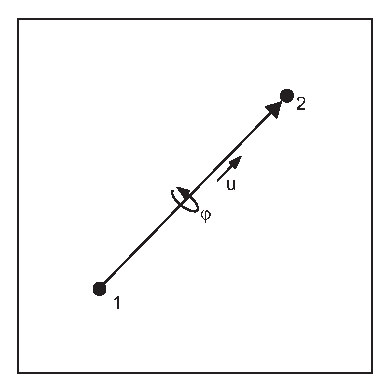
\includegraphics{figures/connetti2}
%DIFDELCMD <         %%%
%DIFDELCMD < \caption{%
{%DIFAUXCMD
\DIFdelFL{Conventional representation of an angular motion of a rotation $\varphi$ around a fixed rotation axis $u$ between 2 frames.}}
        %DIFAUXCMD
%DIFDELCMD < \label{fig:connetti2}
%DIFDELCMD <     \end{minipage}
%DIFDELCMD <     \hfill
%DIFDELCMD <     \begin{minipage}[t]{0.49\textwidth}
%DIFDELCMD <         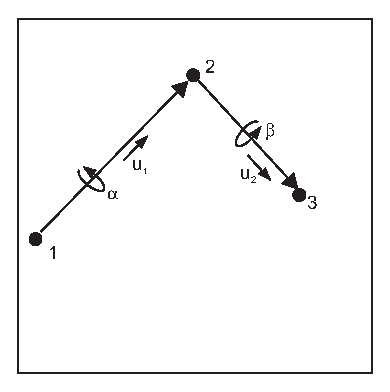
\includegraphics{figures/connetti3}
%DIFDELCMD <         %%%
%DIFDELCMD < \caption{%
{%DIFAUXCMD
\DIFdelFL{Conventional representation of an angular motion from frame (1) to frame (3) passing through frame (2) adopting the strategy of section \ref{subsec:connetti3appr}.}}
        %DIFAUXCMD
%DIFDELCMD < \label{fig:connetti3}
%DIFDELCMD <     \end{minipage}
%DIFDELCMD < \end{figure}
%DIFDELCMD < 

%DIFDELCMD < %%%
\DIFdelend \subsection{Interpolation between 3 poses}
\DIFaddbegin \label{subsec:connetti3}
\DIFaddend If we want to \DIFdelbegin \DIFdel{move }\DIFdelend \DIFaddbegin \DIFadd{rotate }\DIFaddend frame (1) \DIFdelbegin \DIFdel{to }\DIFdelend \DIFaddbegin \DIFadd{into }\DIFaddend frame (3) passing through frame (2), it is possible to adopt twice the strategy of section \ref{subsec:connetti2} (see Fig. \ref{fig:connetti3}). Since in general the unit vectors \DIFdelbegin \DIFdel{$u_1$ and $u_2$ }\DIFdelend \DIFaddbegin \DIFadd{$\vect{u}_1$ and $\vect{u}_2$ }\DIFaddend are different from each other, to preserve the continuity of angular velocity it is necessary to smoothly stop in (2) and then to start again. In the next sections we will present two methodologies to generate the desired motion without the necessity to stop but preserving the velocity and acceleration continuity.

%DIF >  Direct angular motion (2-3 poses)
\DIFaddbegin \begin{figure}[tbp]
    \begin{minipage}[t]{0.49\textwidth}
        \centering
        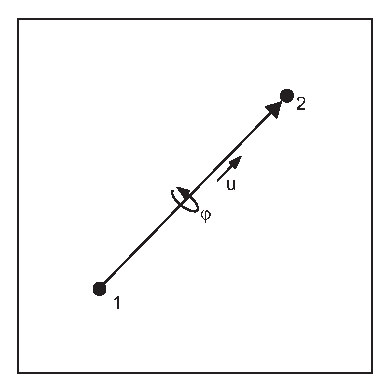
\includegraphics{figures/connetti2}
        \caption{\DIFaddFL{Conventional representation of an angular motion between two frames, consisting in a rotation of angle $\varphi$ about a fixed rotation axis $\vect{u}$. The strategy adopted is described in Section \ref{subsec:connetti2}.}}
        \label{fig:connetti2}
    \end{minipage}
    \hfill
    \begin{minipage}[t]{0.49\textwidth}
        \centering
        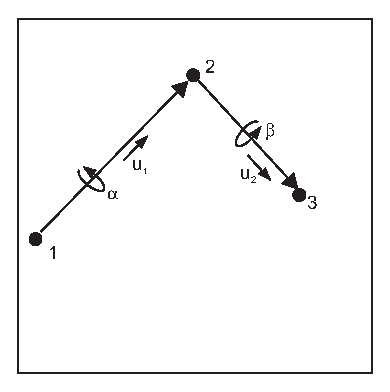
\includegraphics{figures/connetti3}
        \caption{\DIFaddFL{Conventional representation of an angular motion between three frames, starting from frame (1) and ending to frame (3) while passing through frame (2). The strategy adopted is described in Section \ref{subsec:connetti3}.}}
        \label{fig:connetti3}
    \end{minipage}
\end{figure}


\DIFaddend \subsection{Approximate method}
\label{subsec:connetti3appr}
In this section we present a methodology to generate a trajectory from frame (1) to frame (3) passing near frame (2) (Fig. \ref{fig:connetti3a}). This is an approximate solution to our problem.

We initially observe that the frames (2) and (3) can be reached from the previous frames by suitable rotations $\overline{\alpha}$ and $\overline{\beta}$ around suitable axes $\vect{u}_1$ and $\vect{u}_2$
\begin{equation}
    \begin{array}{l}
        R_{02} = R_{01}R_{12} 
        \qquad\qquad 
        R_{12} = \overline{R}(\vect{u}_1,\overline{\alpha})\\[2ex]
        R_{03} = R_{02}R_{23} 
        \qquad\qquad  
        R_{23} = \overline{R}(\vect{u}_2,\overline{\beta})
    \end{array}
    \label{eq:rotA,B}
\end{equation}

%DIF >  Approx interpolation of 3 poses
\begin{figure}[tbp]
    \begin{minipage}[t]{0.49\textwidth}
        \DIFaddbeginFL \centering
        \DIFaddendFL 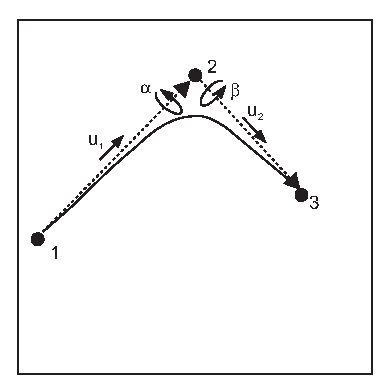
\includegraphics{figures/connetti3a}
        \caption{Approximate \DIFaddbeginFL \DIFaddFL{angular }\DIFaddendFL trajectory between \DIFdelbeginFL \DIFdelFL{3 }\DIFdelendFL \DIFaddbeginFL \DIFaddFL{three }\DIFaddendFL frames (first definition). \DIFaddbeginFL \DIFaddFL{The strategy adopted is described in Section \ref{subsec:connetti3appr}.}\DIFaddendFL }
        \label{fig:connetti3a}
    \end{minipage}
    \hfill
    \begin{minipage}[t]{0.49\textwidth}
        \DIFaddbeginFL \centering
        \DIFaddendFL 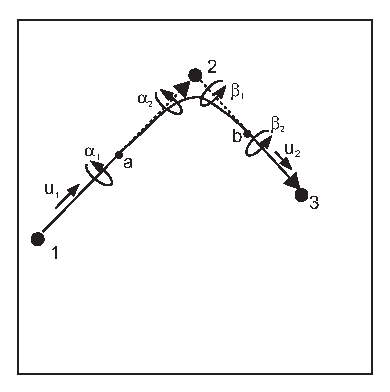
\includegraphics{figures/connetti3b}
        \caption{Approximate \DIFaddbeginFL \DIFaddFL{angular }\DIFaddendFL trajectory between \DIFdelbeginFL \DIFdelFL{3 }\DIFdelendFL \DIFaddbeginFL \DIFaddFL{three }\DIFaddendFL frames (variant \DIFaddbeginFL \DIFaddFL{to pass closer to intermediate frame}\DIFaddendFL ). \DIFaddbeginFL \DIFaddFL{The strategy adopted is described in Section \ref{subsec:connetti3appr}. }\DIFaddendFL See also Fig. \ref{fig:sfera1}}
        \label{fig:connetti3b}
    \end{minipage}
\end{figure}

%DIF >  Motion laws
\begin{figure}[tbp]
    \begin{minipage}[t]{0.49\textwidth}
        \DIFaddbeginFL \centering
        \DIFaddendFL 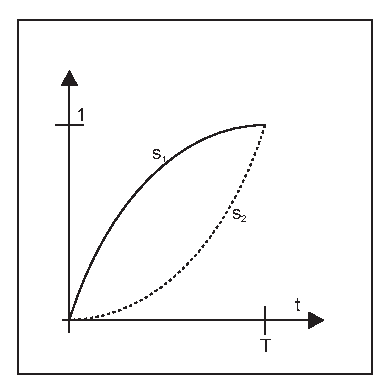
\includegraphics{figures/Legge1}
        \caption{Unitary \DIFdelbeginFL \DIFdelFL{law of }\DIFdelendFL motion \DIFaddbeginFL \DIFaddFL{laws }\DIFaddendFL for the angles $\alpha$ and $\beta$\DIFaddbeginFL \DIFaddFL{, }\DIFaddendFL to be used in the approximate connection of the three frames \DIFaddbeginFL \DIFaddFL{with Eq}\DIFaddendFL . \DIFaddbeginFL \DIFaddFL{\ref{eq:cambiaA,B}.}\DIFaddendFL }
        \label{fig:legge1}
    \end{minipage}
    \hfill
    \begin{minipage}[t]{0.49\textwidth}
        %DIF < \includegraphics{legge1sva}
        \DIFaddbeginFL \centering
        \DIFaddendFL 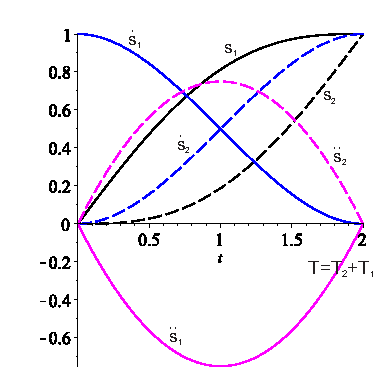
\includegraphics{figures/legge5sva-j}
        \caption{Position, velocity ed acceleration of the \DIFdelbeginFL \DIFdelFL{law of motions }\DIFdelendFL \DIFaddbeginFL \DIFaddFL{motion laws }\DIFaddendFL $s_1$ and $s_2$ \DIFaddbeginFL \DIFaddFL{presented in Fig}\DIFaddendFL . \DIFaddbeginFL \DIFaddFL{\ref{fig:legge1}.}\DIFaddendFL }
        \label{fig:legge1sva}
    \end{minipage}
\end{figure}

So a trajectory from pose (1) to pose (3) can be obtained by the following equation
\begin{equation}
    R = R_{01}\overline{R}(\vect{u}_{1(1)},\alpha)\overline{R}(\vect{u}_{2(2)},\beta) 
    \qquad\qquad 
    % \alpha=0,...,\overline{\alpha}, \beta=0,...,\overline{\beta}
    \alpha \in \left[ 0, \overline{\alpha} \right], \beta \in \left[ 0, \overline{\beta} \right]
    \label{eq:raccordo}
\end{equation}
where for $\alpha=\beta=0$ we get $R=R_{01}$, while for $\alpha=\overline{\alpha}$ and $\beta=\overline{\beta}$ we get  $R=R_{03}$.

To pass near frame (2) it is necessary to assign suitable initial and final conditions to the variation law of  $\alpha$ and $\beta$. Initially it is necessary that $\alpha$ varies quickly and slowly in the final part. Similarly initially $\beta$ should vary slowly and quickly in the final part. As an example consider the following law (Fig. \ref{fig:legge1} and \DIFaddbegin \DIFadd{Fig. }\DIFaddend \ref{fig:legge1sva})
\begin{equation}
    \begin{array}{c}
        \alpha(t) = \overline{\alpha} s_{1}(t)
        \qquad\qquad
        \beta(t)=\overline{\beta} s_{2}(t)
        \qquad\qquad
        % t=0,...,T\\[2ex]
        t \in \left[ 0, T \right] \\[2ex]
        \dot{s}_1(0)>0 \qquad \dot{s}_1(T)=0
        \qquad\qquad
        \ddot{s}_1(0)=\ddot{s}_1(T)=0\\[2ex]
        \dot{s}_2(0)=0 \qquad \dot{s}_2(T)>0
        \qquad\qquad
        \ddot{s}_2(0)=\ddot{s}_2(T)=0
    \end{array}
    \label{eq:cambiaA,B}
\end{equation}

To pass \DIFdelbegin \DIFdel{more close }\DIFdelend \DIFaddbegin \DIFadd{closer }\DIFaddend to pose (2) it is possible to adopt the following strategy (Figure \ref{fig:connetti3b})
\begin{itemize}
    \item perform an initial rotation  $\alpha_1$ around a $\vect{u}_1$ and reach frame \DIFdelbegin \DIFdel{(a)}\DIFdelend \DIFaddbegin \DIFadd{$(a)$}\DIFaddend ,
    \item then move from frame  $(a)$ to $(b)$ using the previously described algorithm shown in Fig. \ref{fig:connetti3a} and Eq. \ref{eq:raccordo} with rotations $\alpha_2$ and $\beta_1$
    \item finally move from frame \DIFdelbegin \DIFdel{(b) to (3) }\DIFdelend \DIFaddbegin \DIFadd{$(b)$ to $(3)$ }\DIFaddend rotating around $\vect{u}_2$ \DIFdelbegin \DIFdel{of }\DIFdelend \DIFaddbegin \DIFadd{by }\DIFaddend an angle $\beta_2$.
\end{itemize}
The mentioned operations are performed assuming $\overline{\alpha}=\alpha_1+\alpha_2$, $\overline{\beta}=\beta_1+\beta_2$.
So the trajectory is generated by the following three steps

\begin{equation}
    \begin{array}{lll}
        step\ 1: & R=R_{01}\overline{R}(\vect{u}_1,\alpha) & \alpha \in [0, \alpha_1]\\

        step\ 2: & R=R_{01}\overline{R}(\vect{u}_1,\alpha_1)\overline{R}(\vect{u}_1,\alpha)\overline{R}(\vect{u}_2,\beta) & \alpha \in [0, \alpha_2], \beta \in [0,\beta_1]\\

        step\ 3: &
        R=R_{01}\overline{R}(\vect{u}_1,\overline{\alpha})\overline{R}(\vect{u}_2,\beta_1)\overline{R}(\vect{u}_2,\beta) & \beta \in [0, \beta_2]
    \end{array}
    \label{eq:3step}
\end{equation}

In practice steps 1 and 3 are classical SLERP interpolations segments smoothly connected by step 2. The adoption of the law of motions similar to those of Figure  \ref{fig:legge1sva} guarantees continuity of velocity and acceleration in the connection points (a) and (b) if the following  conditions are assigned
\begin{equation}
    \begin{array}{lcl}
        s_1(0)= 0 && s_2(0)=0\\
        \dot{s}_1(0)=\dot{\overline{\alpha}} && \dot{s}_2(0)=0 \\
        \ddot{s}_1(0)=0 && \ddot{s}_2(0)=0\\
        s_1(T)= \alpha_2 && s_2(T)=\beta_1\\
        \dot{s}_1(T)=0 && \dot{s}_2(T)=\dot{\overline{\beta}} \\
        \ddot{s}_1(T)=0 && \ddot{s}_2(T)=0
    \end{array}
    \label{eq:limits}
\end{equation}
where $\dot{\overline{\alpha}}$ and $\dot{\overline{\beta}}$ are, respectively, the angular velocity during the first and third step of the motion. These conditions can be easily obtained by the polynomial law described in section \ref{app:poly5}.
By assuming $s_1+s_2=k t$ and so $s_2=kt-s_1$, $\dot{s}_2=k-\dot{s}_1$, $\ddot{s}_2=-\ddot{s}_1$ for the particular law adopted $s_2(t)=s_1(T-t)$. Moreover $s_1(0)=0$, $\dot{s}_1(0)=1$, $\ddot{s}_1(0)=0$, $s_1(T)=1$,  $\dot{s}_1(T)=0$, $\ddot{s}_1(T)=0$ (see \DIFdelbegin \DIFdel{section }\DIFdelend \ref{app:poly5}). 

A numerical example \DIFaddbegin \DIFadd{of the exposed procedure }\DIFaddend is presented in Fig. \ref{fig:legnani_approx_compo} and Fig. \ref{fig:legnani_approx_vel}. The law of motion can be adjusted to obtain constant angular velocity as shown in Fig. \ref{fig:raccordo3-qNorm} and Fig. \ref{fig:raccordo3-wNorm}.

To generate the motion with constant velocity it is possible to adopt the following numerical approach. The motion description of \DIFdelbegin \DIFdel{figure }\DIFdelend \DIFaddbegin \DIFadd{Figure }\DIFaddend \ref{fig:legnani_approx_compo} is sampled at predefined time intervals $i=0, 1, 2,\ldots n$ then, for any time interval, the absolute value of the angular rotation is evaluated. Finally the absolute time $t_i$ for the $i-th$ sampled orientation is determined as
\begin{equation}
    \begin{array}{l}
        t_0=0\\
        t_i=t_{i-1}+\cfrac{\Delta\varphi_i}{\norm{\vect{\omega}}}
    \end{array}
    \DIFaddbegin \label{eq:deltaT}
\DIFaddend \end{equation}
where $\Delta\varphi_i$ is the angular rotation in the $i-th$ interval (between the time instant $i$ and $i-1$) and $\norm{\vect{\omega}}$ is the desired angular velocity ($\norm{\vect{\omega}}$=1 for the example of Fig. \ref{fig:raccordo3-qNorm} and Fig. \ref{fig:raccordo3-wNorm}). The proposed methodology can be simply adapted to any velocity profile by assigning the required value of $\norm{\vect{\omega}}$ as a function of time. For example it is possible to start the motion with null velocity, increase it until a predefined value is reached and slowing down to smoothly stop at the end of the motion.

% Legnani approx between 3 poses
\begin{figure}[tbp]
    \begin{minipage}[t]{0.49\textwidth}
        \DIFaddbeginFL \centering
        \DIFaddendFL 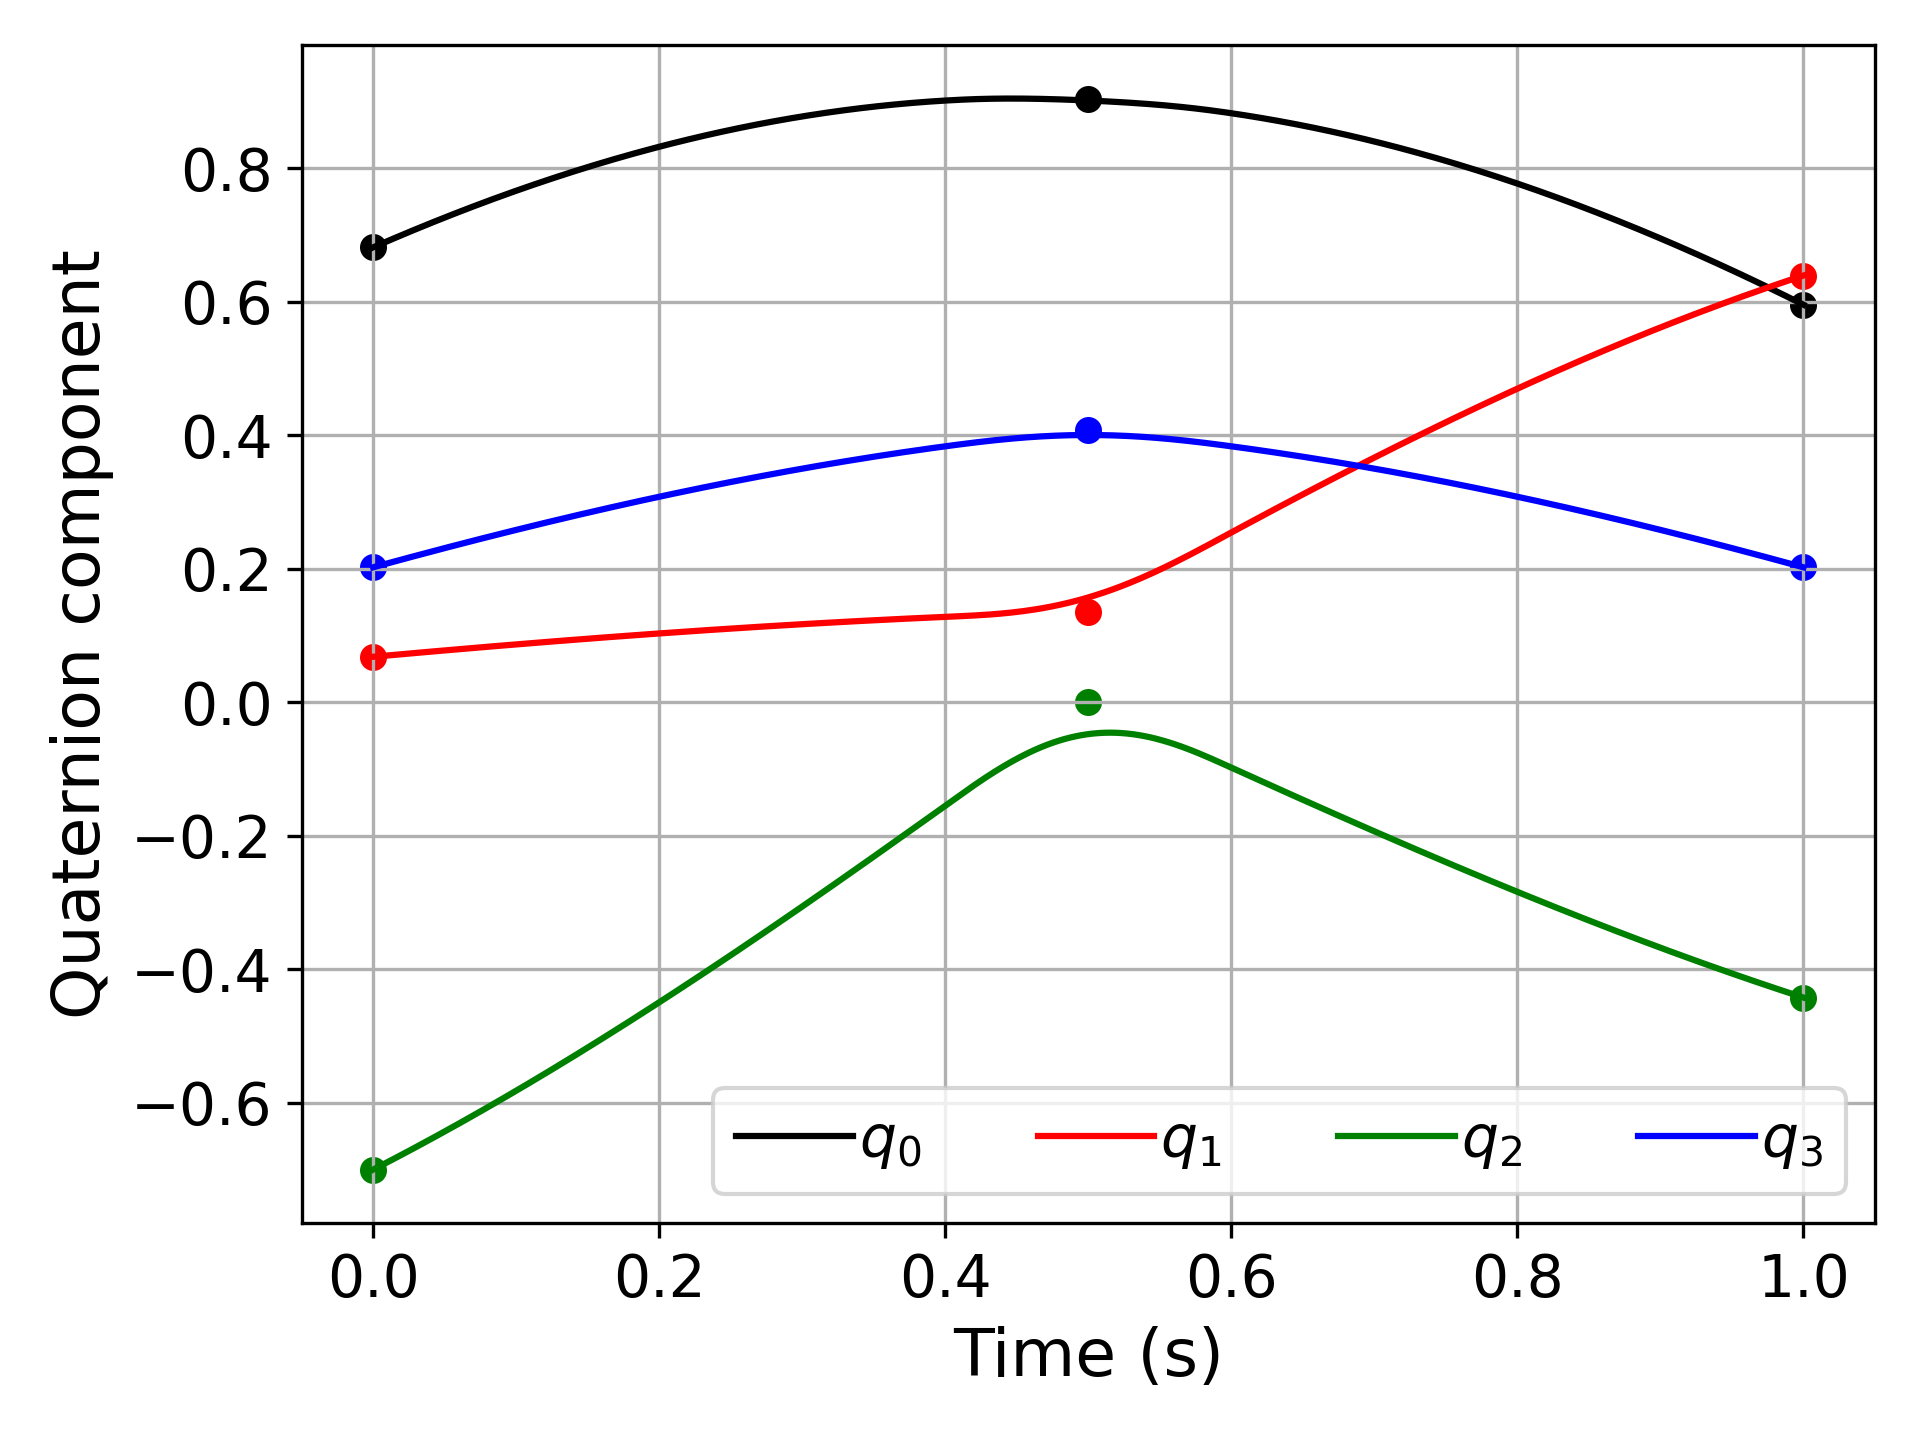
\includegraphics[width=6.5cm]{figures/legnani_approx_compo.png}
        \caption{Numerical example of a trajectory connecting two poses \DIFaddbeginFL \DIFaddFL{and }\DIFaddendFL passing near to an intermediate pose (quaternion components versus time). \DIFaddbeginFL \DIFaddFL{The strategy adopted is described in \ref{subsec:connetti3appr}.}\DIFaddendFL }
        \label{fig:legnani_approx_compo}
    \end{minipage}
    \hfill
    \begin{minipage}[t]{0.49\textwidth}
        \DIFaddbeginFL \centering
        \DIFaddendFL 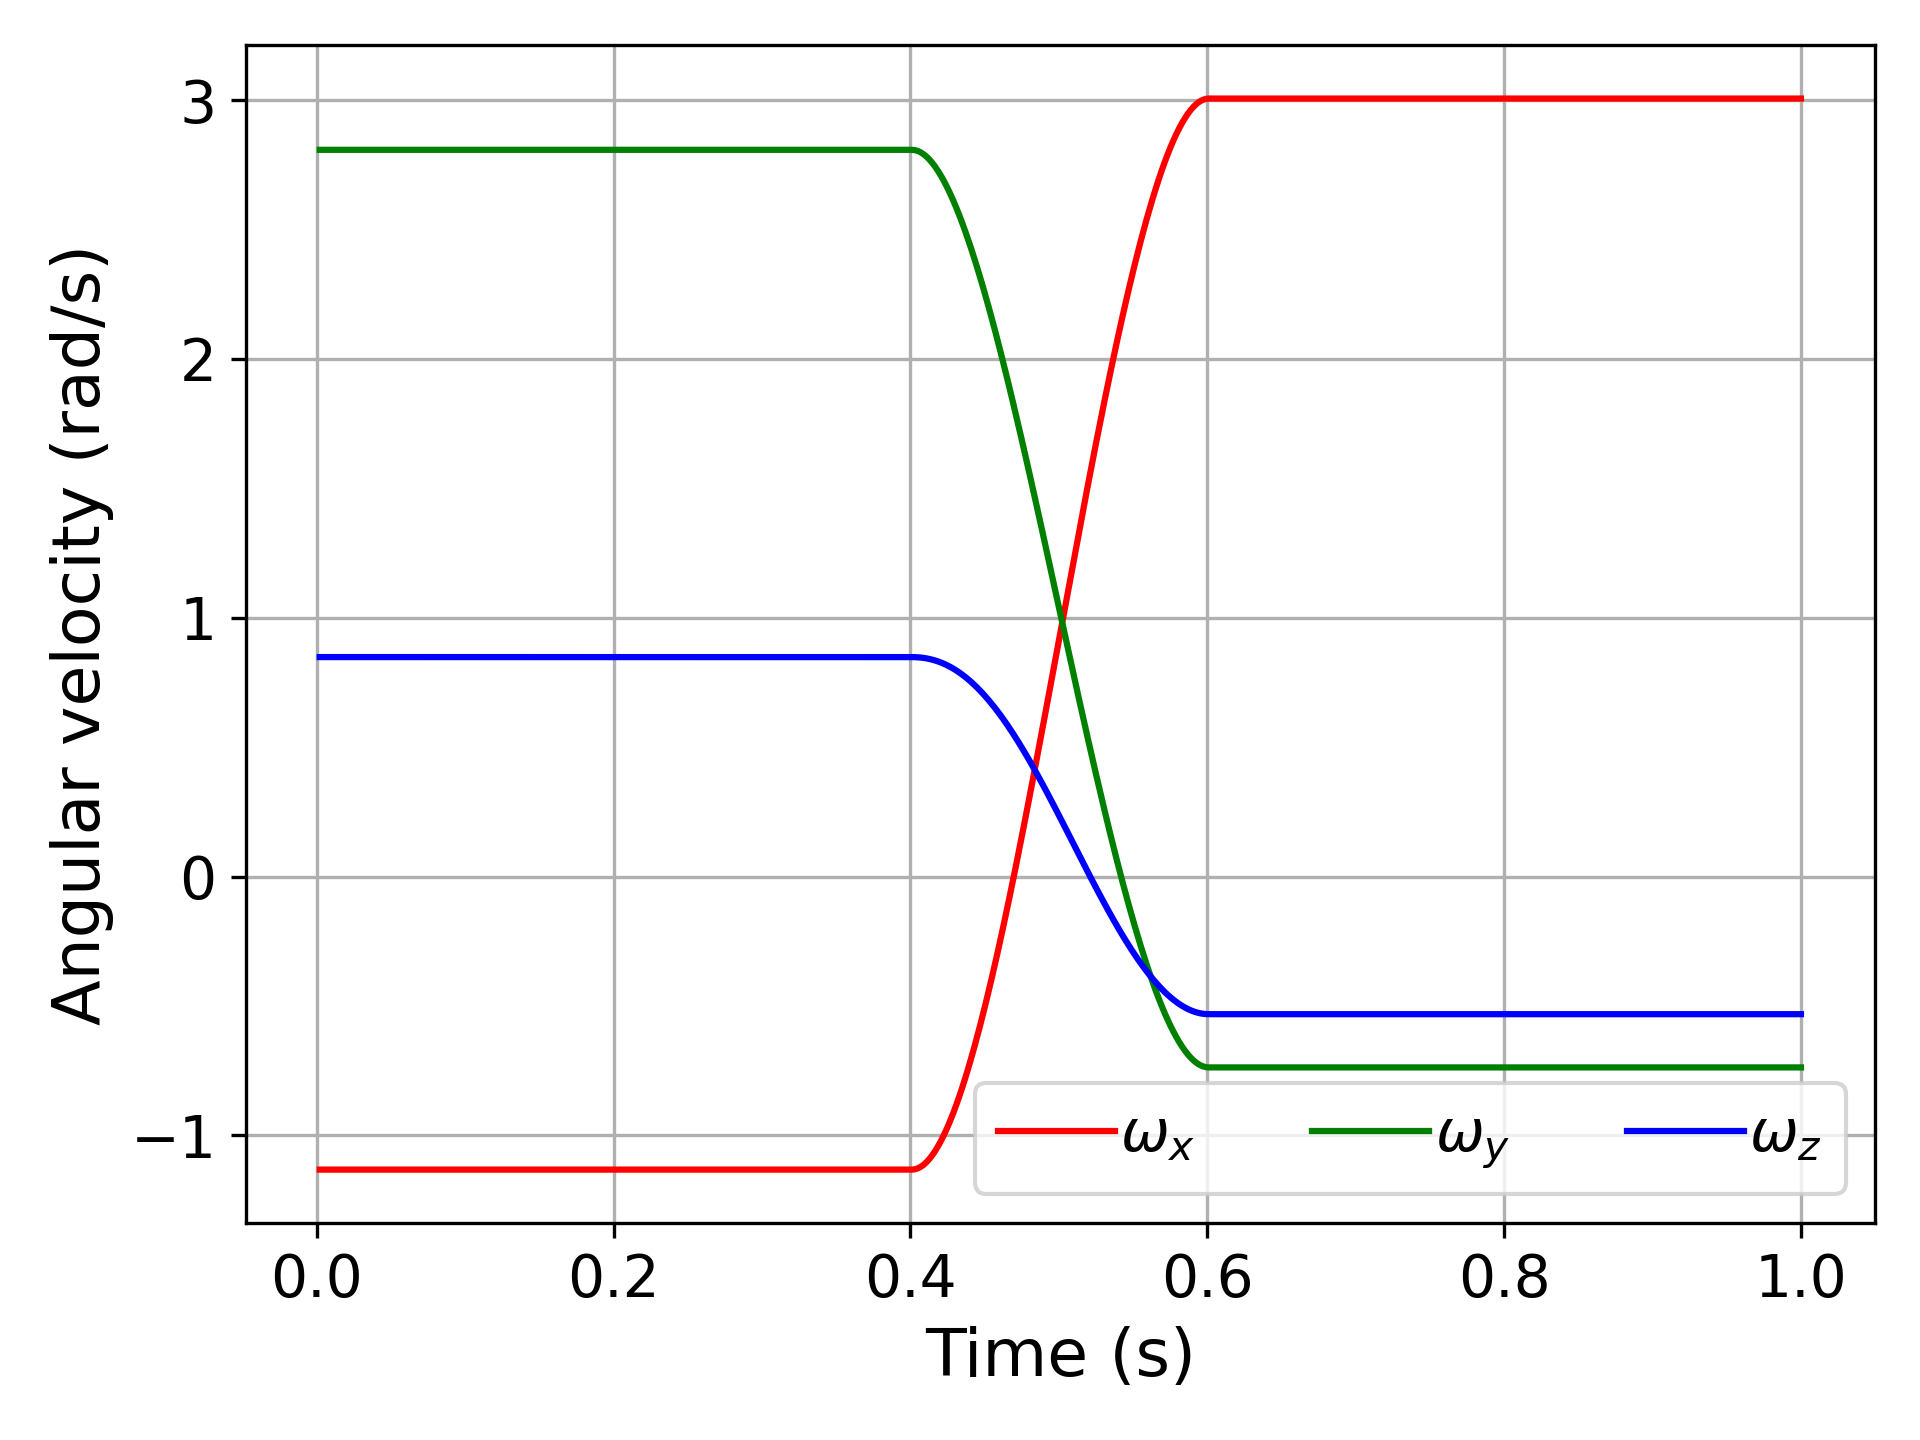
\includegraphics[width=6.5cm]{figures/legnani_approx_vel.png}
        \caption{Angular velocity of interpolation method shown in Fig. \ref{fig:legnani_approx_compo}.}
        \label{fig:legnani_approx_vel}
    \end{minipage}
\end{figure}

% Legnani approx constant vel between 3 poses
\begin{figure}[tbp]
    \begin{minipage}[t]{0.49\textwidth}
        \DIFaddbeginFL \centering
        \DIFaddendFL 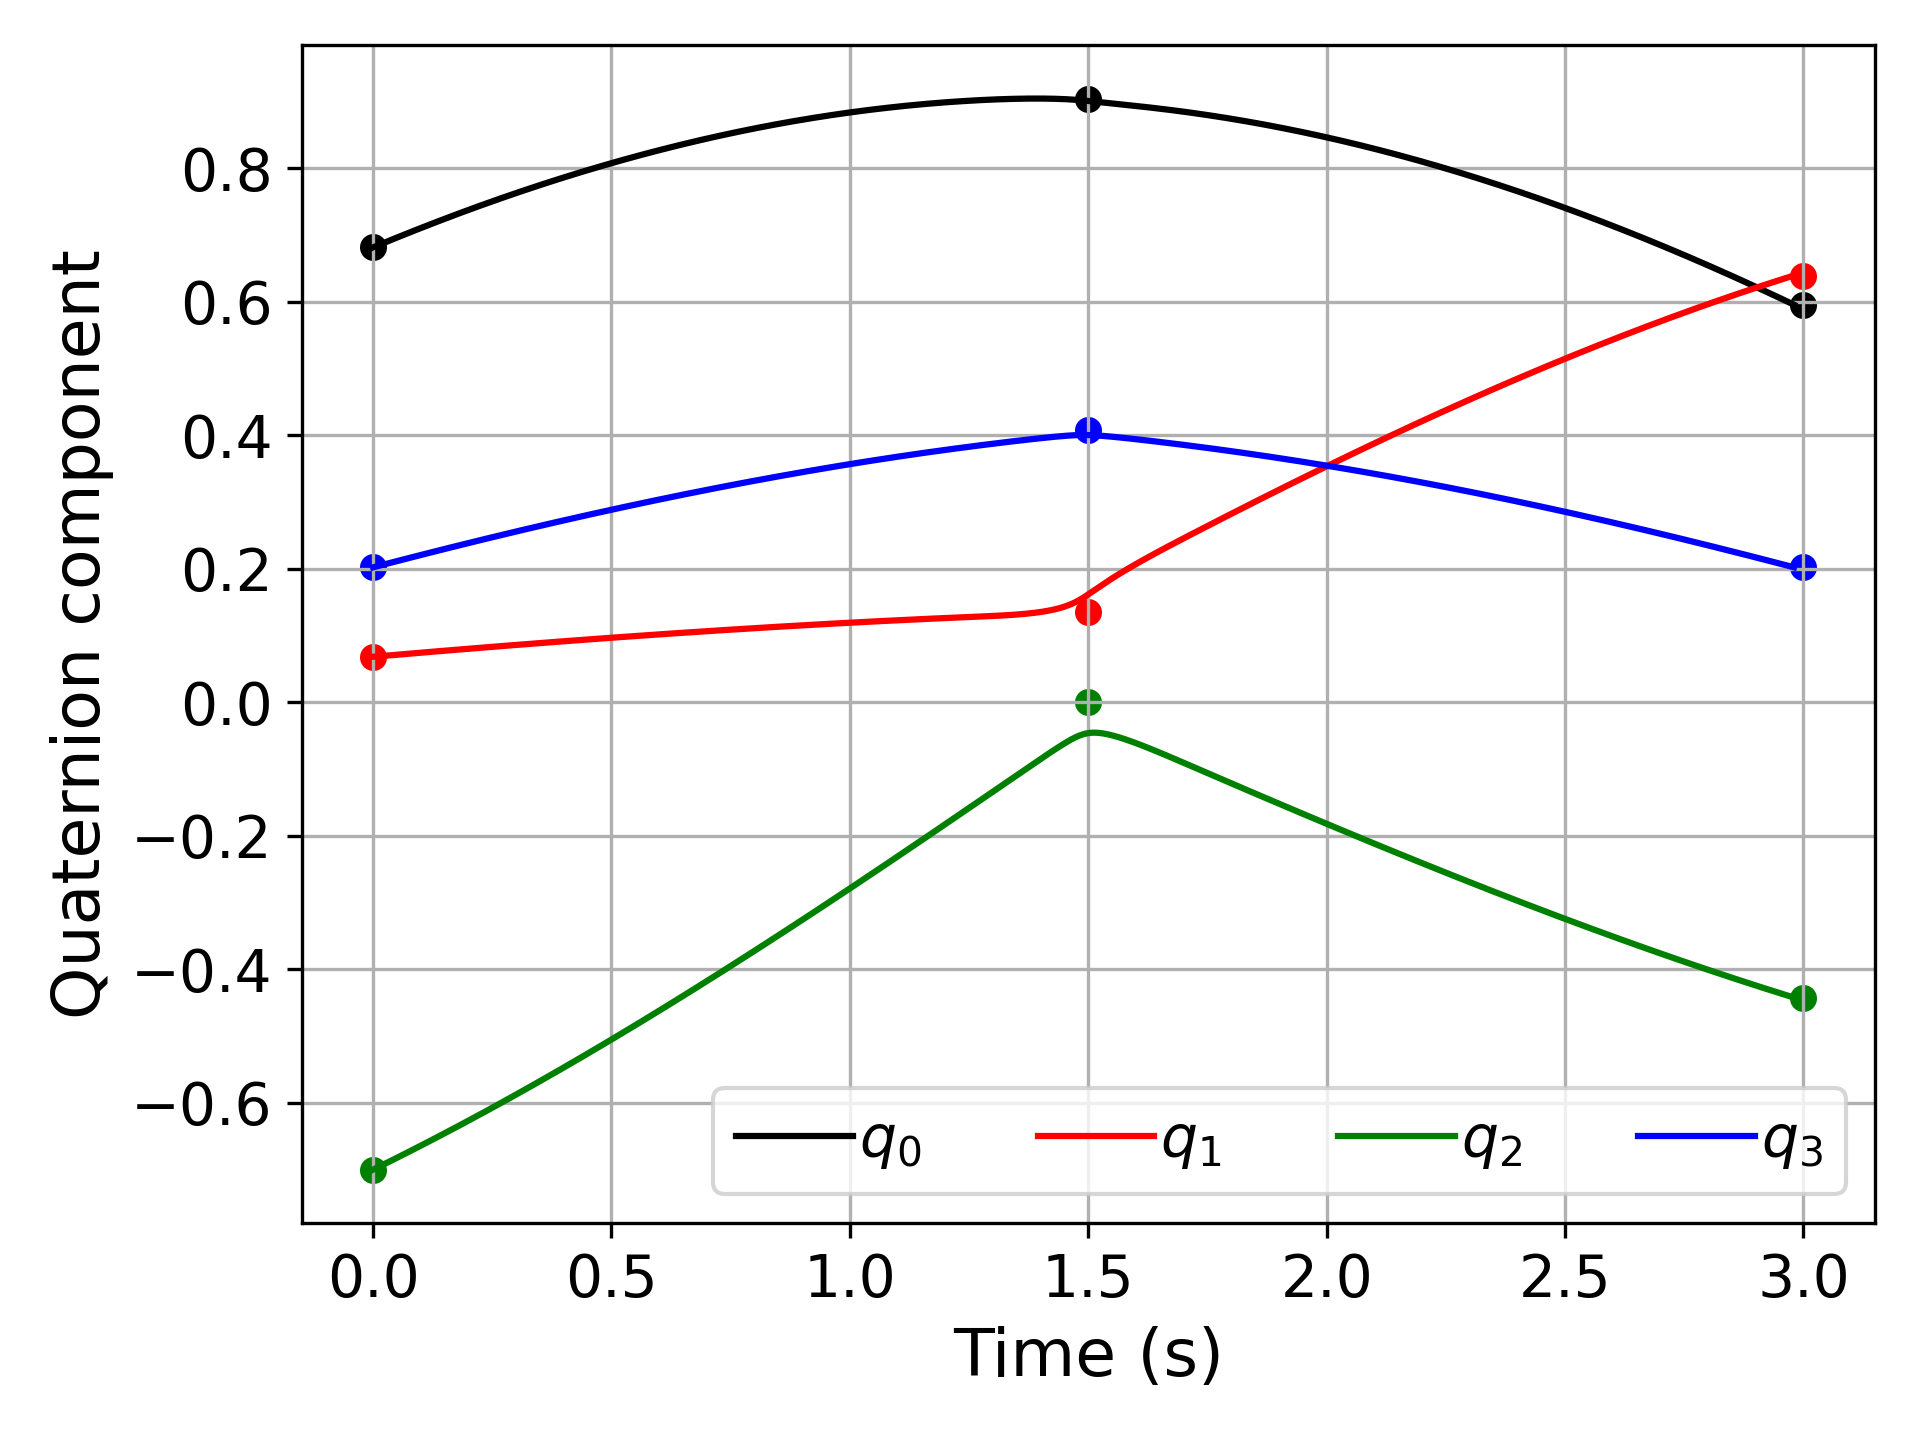
\includegraphics[width=6.5cm]{figures/legnani_constvel_compo.png}
        %DIF <  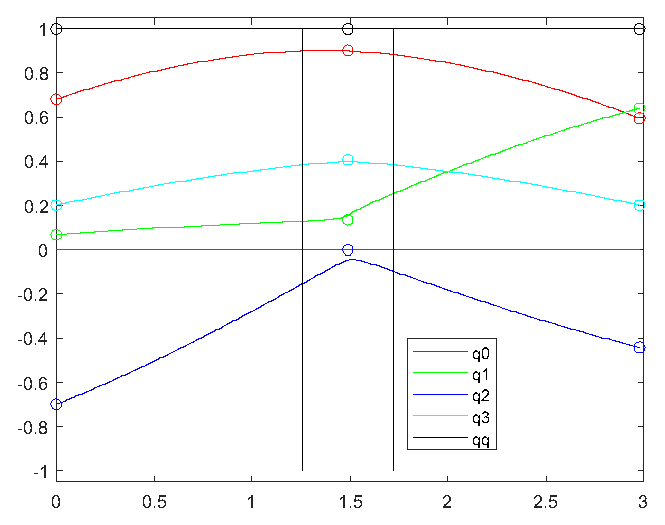
\includegraphics[width=6cm]{figures/raccordo3-qNorm}
        \caption{Numerical example of a trajectory connecting two poses \DIFaddbeginFL \DIFaddFL{and }\DIFaddendFL passing near to an intermediate pose, with constant angular velocity (quaternion components versus time). \DIFaddbeginFL \DIFaddFL{The strategy adopted is described in \ref{subsec:connetti3appr}.}\DIFaddendFL }
        \label{fig:raccordo3-qNorm}
    \end{minipage}
    \hfill
    \begin{minipage}[t]{0.49\textwidth}
        \DIFaddbeginFL \centering
        \DIFaddendFL 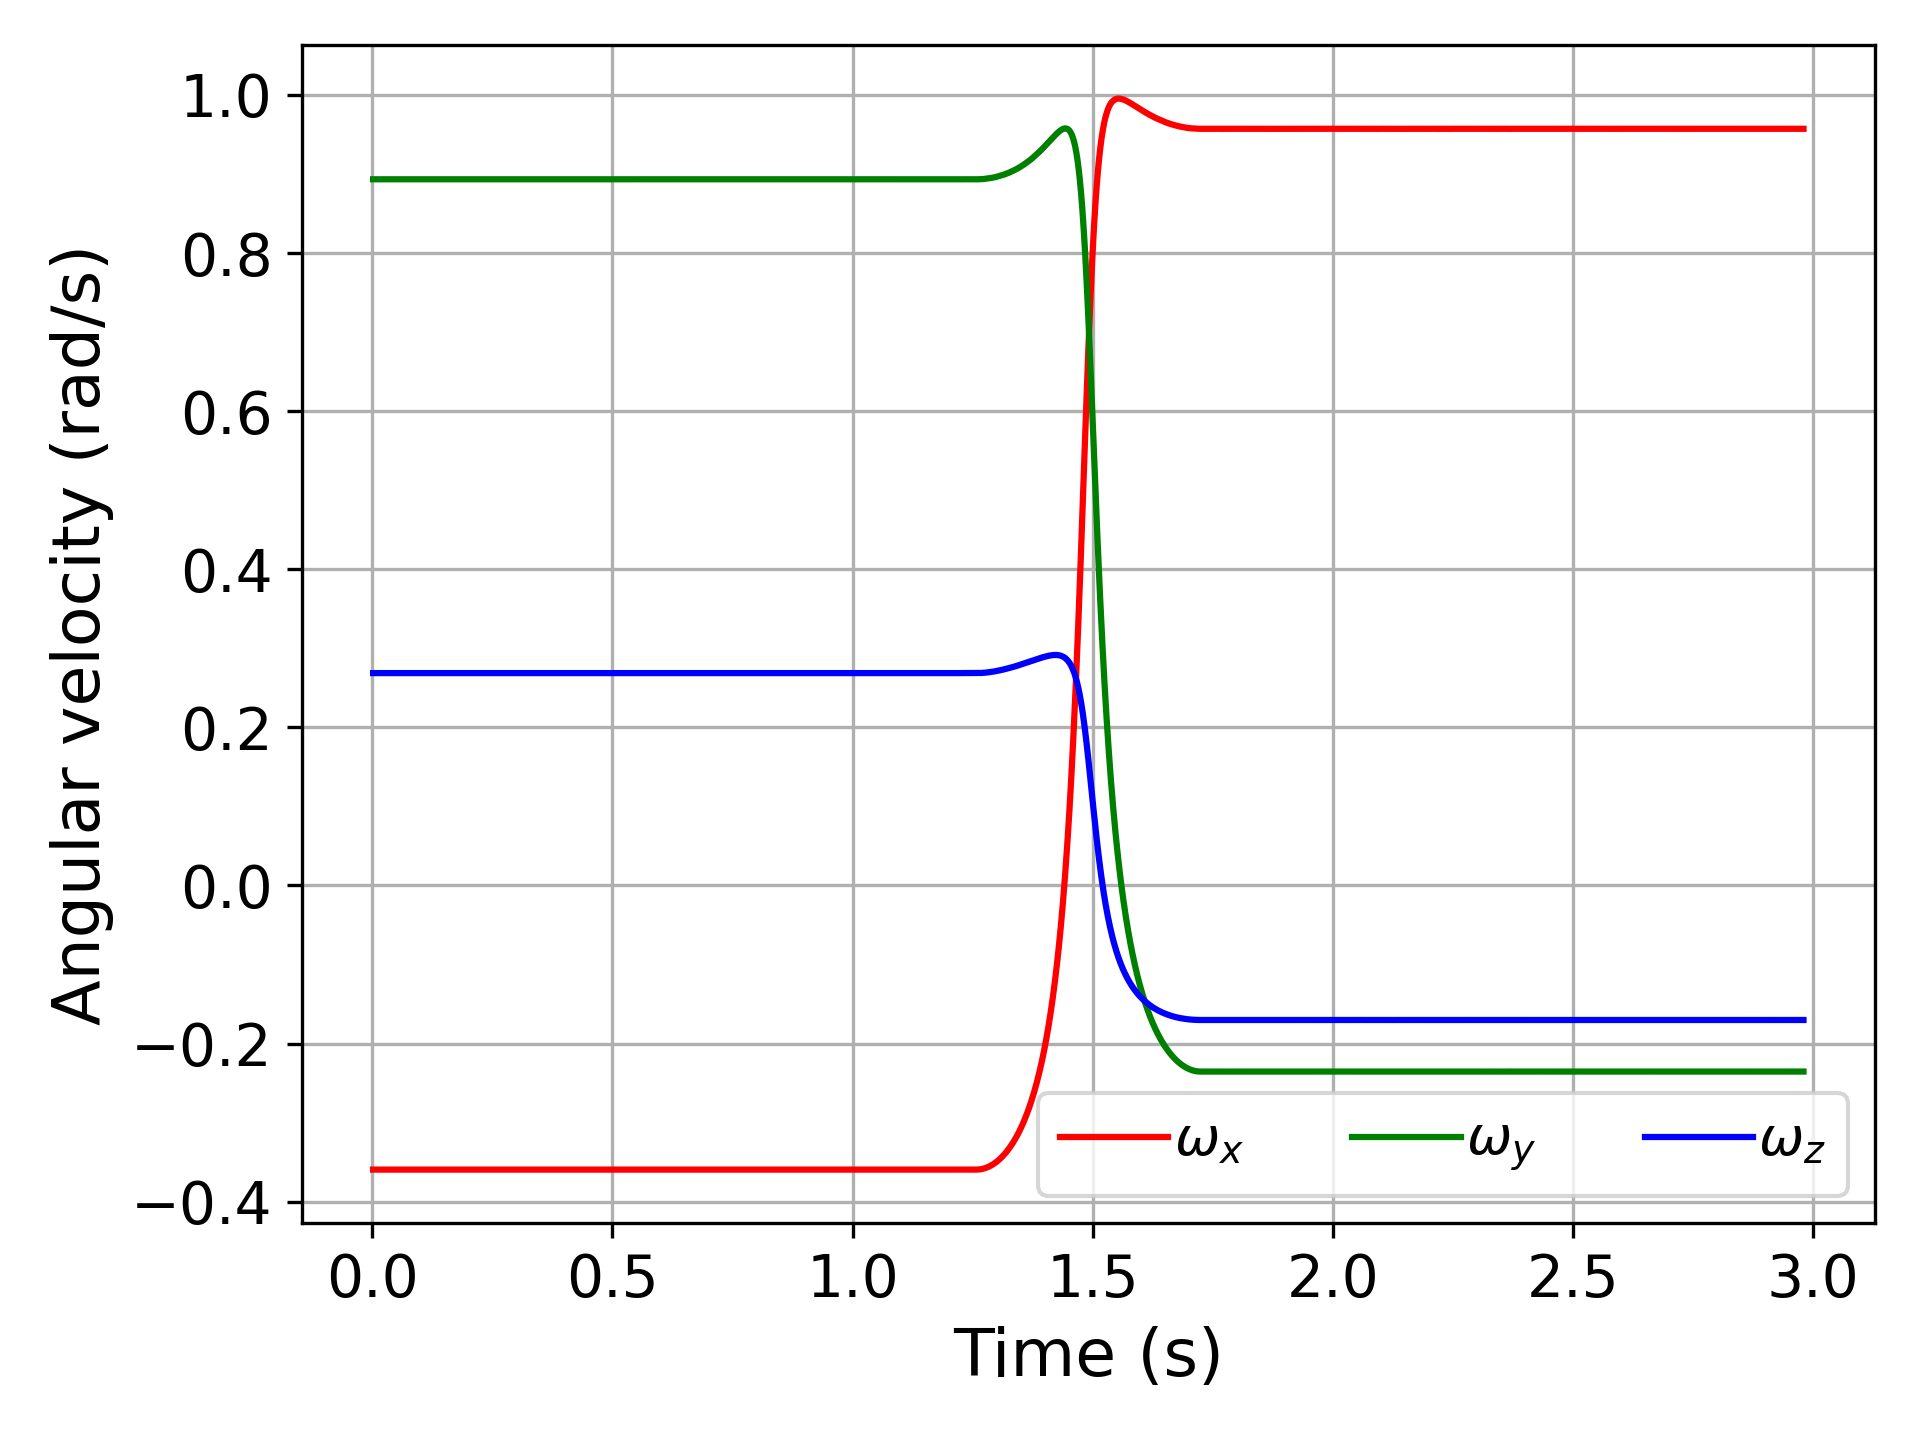
\includegraphics[width=6.5cm]{figures/legnani_constvel_vel.png}
        %DIF <  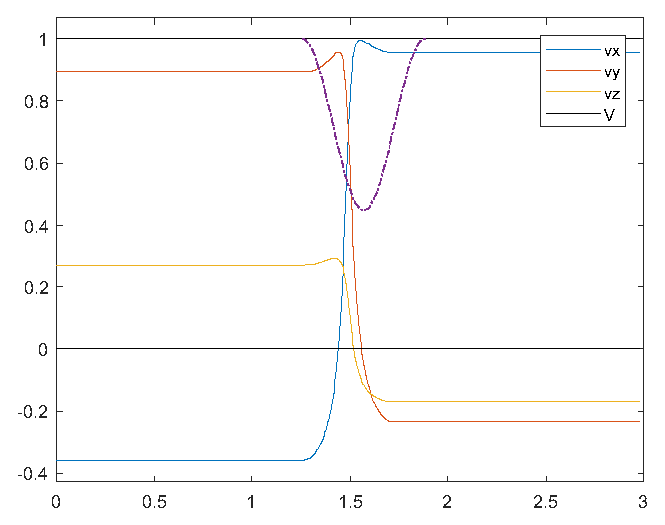
\includegraphics[width=6cm]{figures/raccordo3-wNorm}
        \caption{Angular velocity of interpolation method shown in Fig. \ref{fig:raccordo3-qNorm}.}
        \label{fig:raccordo3-wNorm}
    \end{minipage}
\end{figure}


\subsection{Exact method}
\label{subsec:connetti3esatto}
In order to generate a trajectory that rotates from frame (1) to (3) and passes exactly through frame (2), it is possible to apply twice the algorithm  seen in Section \ref{subsec:connetti3appr}.

At first (see Fig. \ref{fig:connetti3esatto}), a suitable rotation axis $\vect{u}_r$ is chosen to be between $\vect{u}_1$ and $\vect{u}_2$ by using positive arbitrary weights $k_1$ and $k_2$
\begin{equation}
    \vect{u}_r= \cfrac{k_1 \vect{u}_1 + k_2 \vect{u}_2}{\norm{k_1 \vect{u}_1 + k_2 \vect{u}_2}}
    \DIFdelbegin %DIFDELCMD < \label{eq:ur}
%DIFDELCMD < %%%
\DIFdelend %DIF > \label{eq:ur}
    \DIFaddbegin \label{eq:Ur}
\DIFaddend \end{equation}
and, chosen suitable rotation value  $\alpha'$ e $\beta'$ it is possible to generate the frames $(a')$ e $(b')$ by rotation around the axis $\vect{u}_r$. The intermediate auxiliary poses are determined as
\begin{equation}
    R_{0a'}=R(\vect{u}_r,-\alpha')R_{02} 
    \qquad\qquad   
    R_{0b'}=R(\vect{u}_r,\beta')R_{02}
    \label{eq:auxiliary}
\end{equation}
Then it is possible to apply twice the described algorithm: the first time along the poses $(1)-(a')-(2)$ and then along $(2)-(b')-(3)$. A comparison between the approximate and the exact algorithm is presented on the unitary sphere in Fig. \ref{fig:sfera1} and Fig. \ref{fig:sfera2}, while a numerical example is reported in Fig. \ref{fig:q3_legnani_exact} and Fig. \ref{fig:q3_legnani_exact_velocity}.


%DIF <  Schematic exact/extended exact method concept
\DIFdelbegin %DIFDELCMD < \begin{figure}[tbp]
%DIFDELCMD <     \begin{minipage}[t]{0.49\textwidth}
%DIFDELCMD <         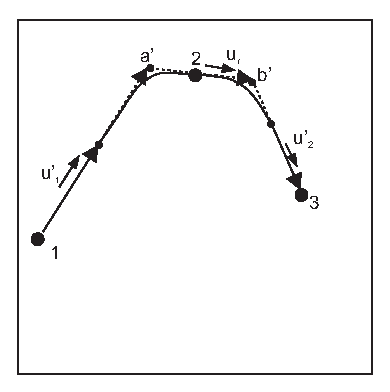
\includegraphics{figures/connetti3esatto}
%DIFDELCMD <         %%%
%DIFDELCMD < \caption{%
{%DIFAUXCMD
\DIFdelFL{Exact trajectory connecting three different frames by using the intermediate poses $(a')$ and $(b')$; see also Fig. \ref{fig:sfera2}}}
        %DIFAUXCMD
%DIFDELCMD < \label{fig:connetti3esatto}
%DIFDELCMD <     \end{minipage}
%DIFDELCMD <     \hfill
%DIFDELCMD <     \begin{minipage}[t]{0.49\textwidth}
%DIFDELCMD <         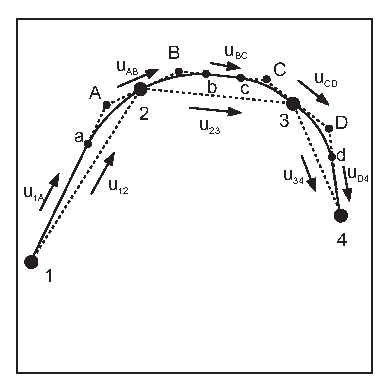
\includegraphics[width=6cm]{figures/connetti4esatto.eps}
%DIFDELCMD <         %%%
%DIFDELCMD < \caption{%
{%DIFAUXCMD
\DIFdelFL{Exact trajectory connecting four different frames by using the intermediate poses $(A)$, $(B)$, $(C)$ and $(D)$}}
        %DIFAUXCMD
%DIFDELCMD < \label{fig:legnani_general_method}
%DIFDELCMD <     \end{minipage}
%DIFDELCMD < \end{figure}
%DIFDELCMD < 

%DIFDELCMD < %%%
%DIF <  Unit sphere representation of approx/exact Legnani
%DIFDELCMD < \begin{figure}[tbp]
%DIFDELCMD <     \begin{minipage}[t]{0.49\textwidth}
%DIFDELCMD <         %%%
%DIF < 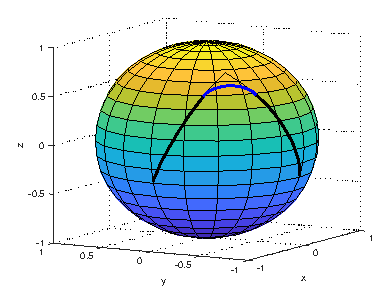
\includegraphics{figures/sfera1}
        %DIFDELCMD < 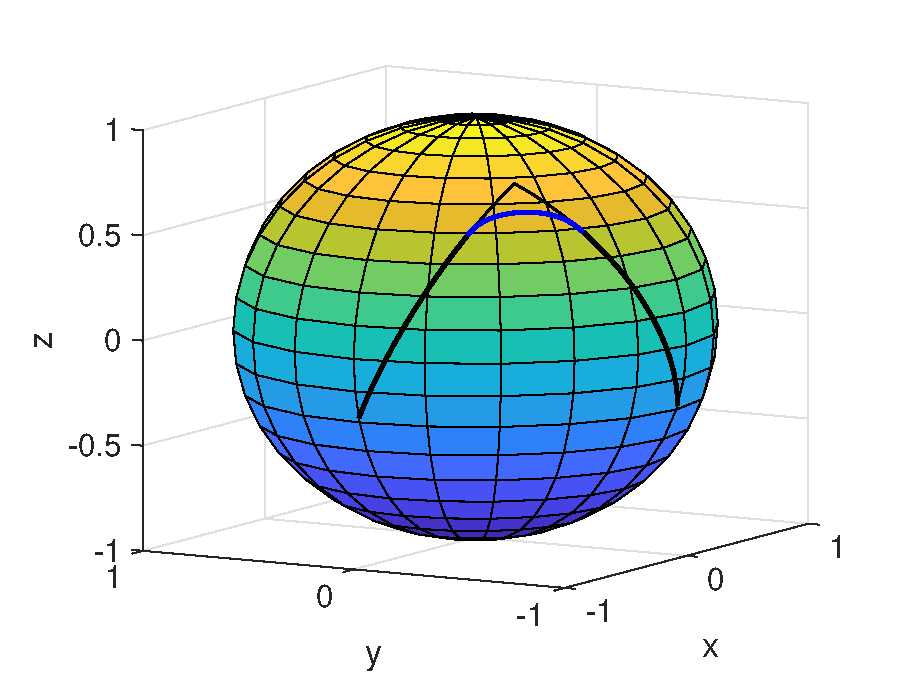
\includegraphics[width=0.95\textwidth]{figures/sfera1a}
%DIFDELCMD <         %%%
%DIFDELCMD < \caption{%
{%DIFAUXCMD
\DIFdelFL{Representation on the unitary sphere of the approximate algorithm (cfr Fig. \ref{fig:connetti3b}).}}
        %DIFAUXCMD
%DIFDELCMD < \label{fig:sfera1}
%DIFDELCMD <     \end{minipage}
%DIFDELCMD <     \hfill
%DIFDELCMD <     \begin{minipage}[t]{0.49\textwidth}
%DIFDELCMD <         %%%
%DIF < \includegraphics{legge1sva}
        %DIF < 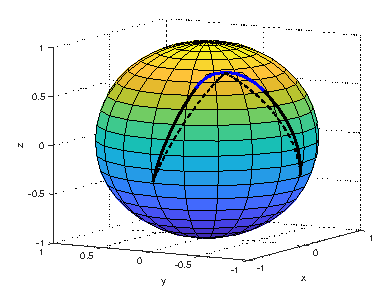
\includegraphics{figures/sfera2}
        %DIFDELCMD < 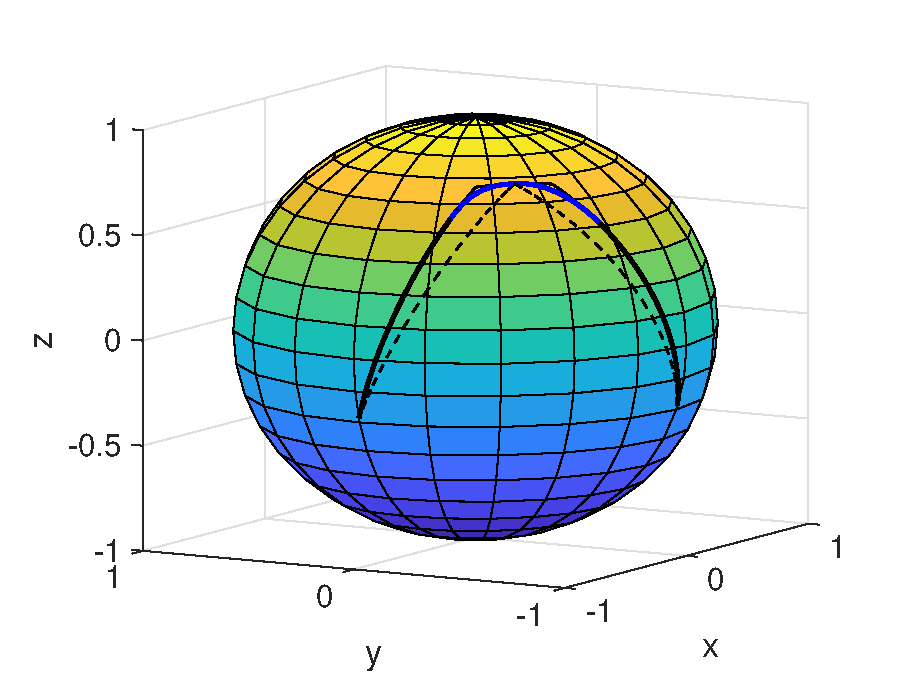
\includegraphics[width=0.95\textwidth]{figures/sfera2a}
%DIFDELCMD <         %%%
%DIFDELCMD < \caption{%
{%DIFAUXCMD
\DIFdelFL{Representation on the unitary sphere of the exact algorithm (cfr Fig. \ref{fig:connetti3esatto}).}}
        %DIFAUXCMD
%DIFDELCMD < \label{fig:sfera2}
%DIFDELCMD <     \end{minipage}  
%DIFDELCMD < \end{figure}
%DIFDELCMD < 

%DIFDELCMD < %%%
%DIF <  Numerical example of 3 quat interp: Legnani exact (q and w)
%DIFDELCMD < \begin{figure}[tbp]
%DIFDELCMD <     \begin{minipage}[t]{0.49\textwidth}
%DIFDELCMD <         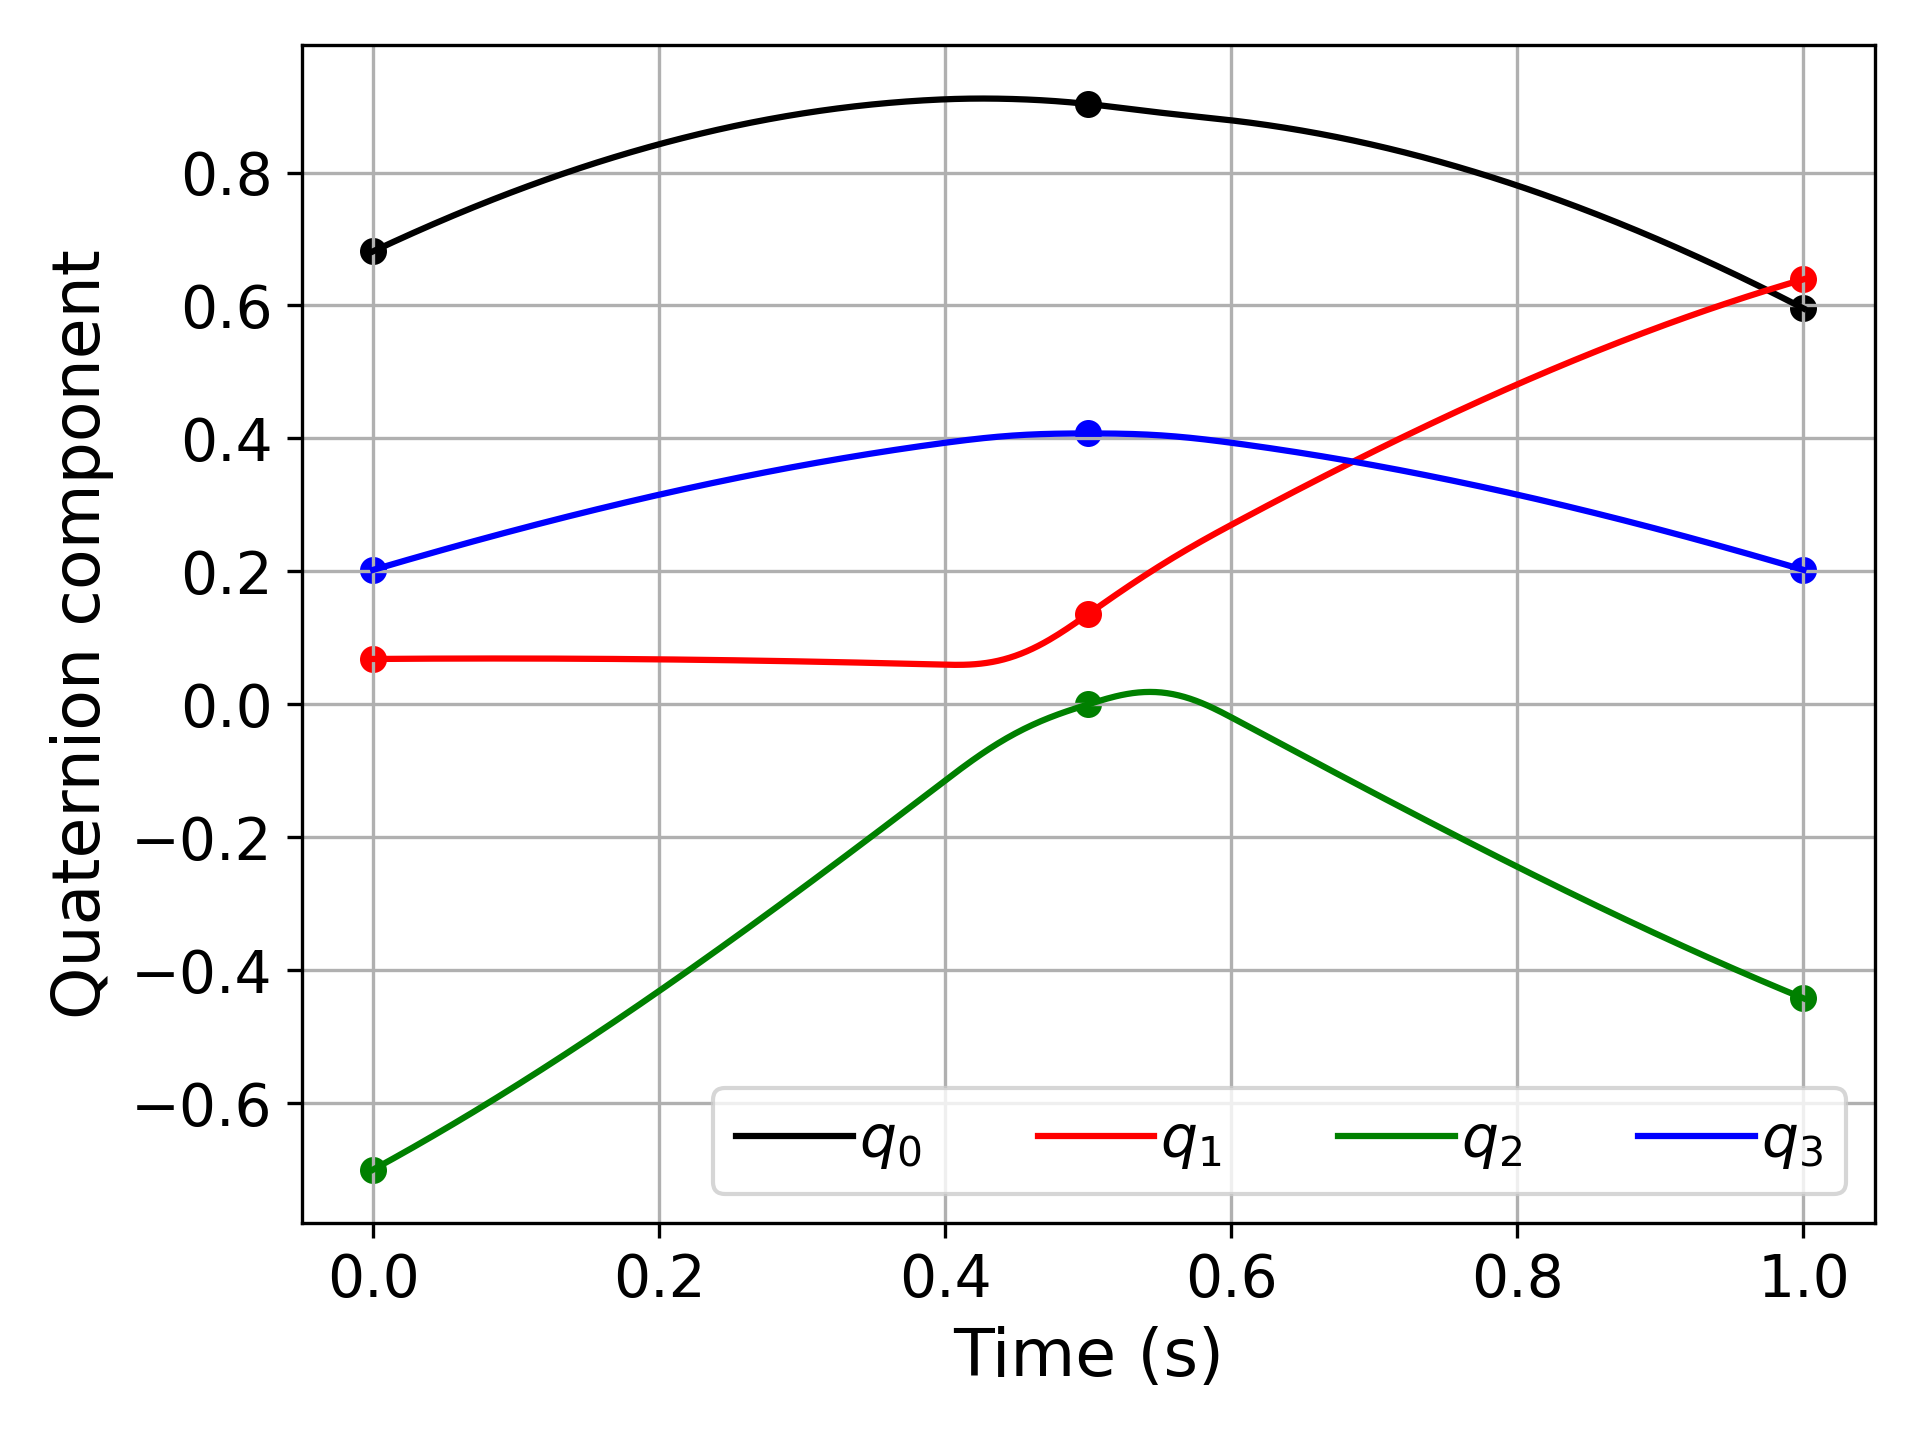
\includegraphics[width=6.5cm]{figures/legnani_exact_compo.png}
%DIFDELCMD <         %%%
%DIFDELCMD < \caption{%
{%DIFAUXCMD
\DIFdelFL{Numerical example of a trajectory connecting two poses and passing exactly through an intermediate pose (quaternion components versus time).}}
        %DIFAUXCMD
%DIFDELCMD < \label{fig:q3_legnani_exact}
%DIFDELCMD <     \end{minipage}
%DIFDELCMD <     \hfill
%DIFDELCMD <     \begin{minipage}[t]{0.49\textwidth}
%DIFDELCMD <         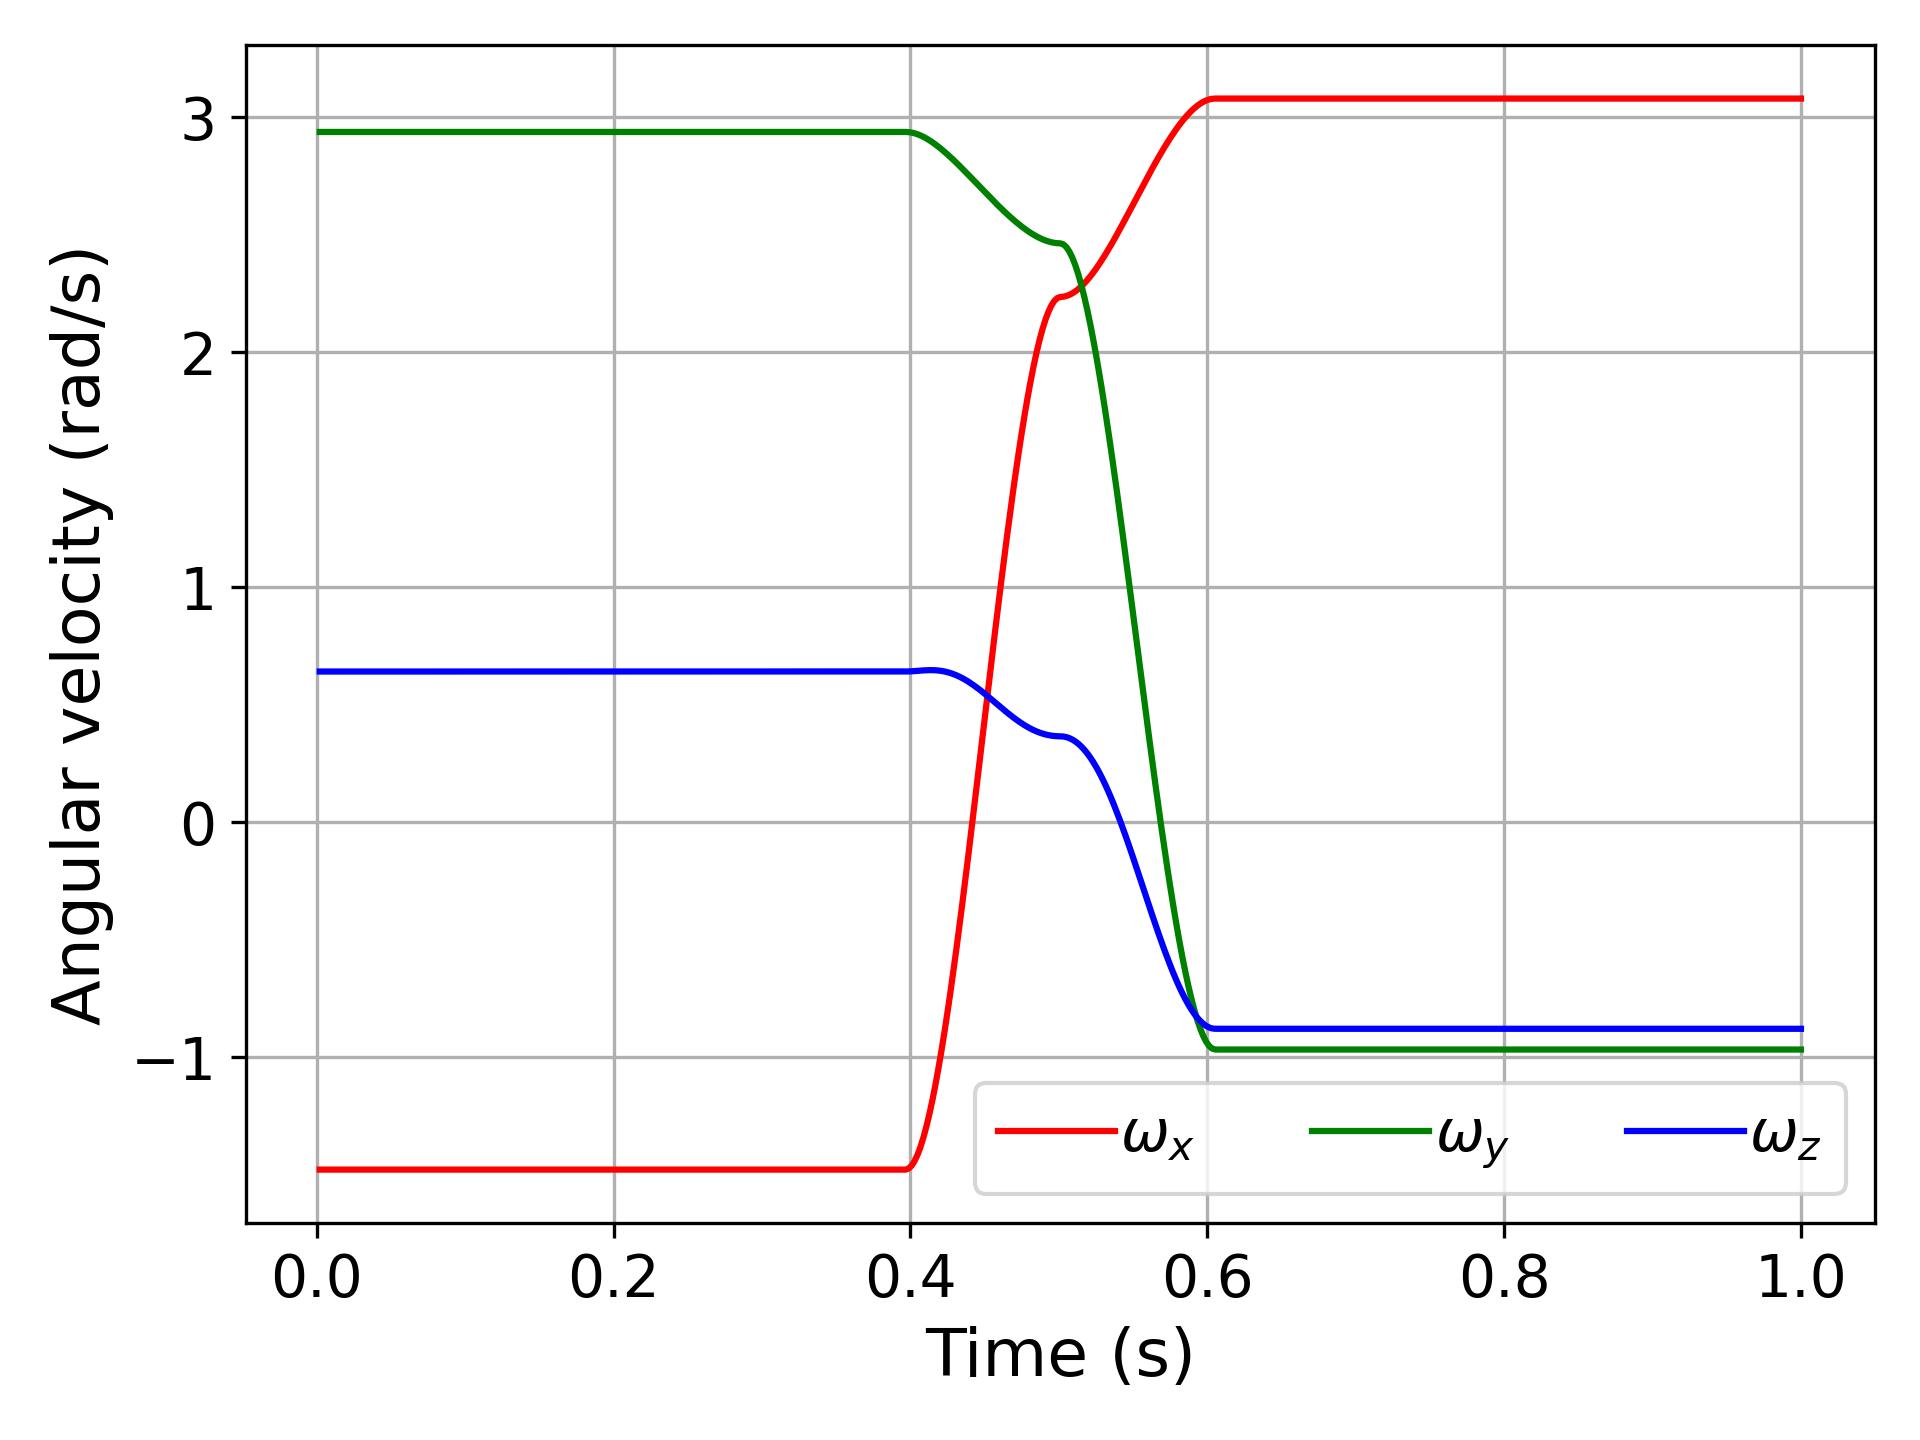
\includegraphics[width=6.5cm]{figures/legnani_exact_vel.png}
%DIFDELCMD <         %%%
%DIFDELCMD < \caption{%
{%DIFAUXCMD
\DIFdelFL{Angular velocity of interpolation method shown in Fig. \ref{fig:q3_legnani_exact}.}}
        %DIFAUXCMD
%DIFDELCMD < \label{fig:q3_legnani_exact_velocity}
%DIFDELCMD <     \end{minipage}
%DIFDELCMD < \end{figure}
%DIFDELCMD < 

%DIFDELCMD < %%%
\DIFdelend \subsection{Exact method for \DIFdelbegin \DIFdel{N }\DIFdelend \DIFaddbegin \DIFadd{arbitrary number of }\DIFaddend rotations}
\DIFaddbegin \label{subsec:connetti_esatto_general}
\DIFaddend The presented exact algorithm can be extended to interpolate an arbitrary number of rotations. For each intermediate frame $(i)$, i.e. from $(2)$ to $(N-1)$, the fillet rotation axes are computed by weighted average of the axes connecting $(i)$ with $(i-1)$ and $(i+1)$. Next, the auxiliary poses $(A)$, $(B)$, $(C)$, \ldots, $(X)$ (see Fig. \ref{fig:legnani_general_method}) are chosen on the fillet axes by rotating of suitable desired angles. Finally, it is possible to compute the axes $\vect{u}_{1A}$, $\vect{u}_{BC}$, $\vect{u}_{D4}$, \ldots, $\vect{u}_{X-1, X}$ and introduce the additional knots $(a)$, $(b)$, $(c)$, \ldots, $(x)$ at desired angular position. For example, assuming 4 input rotations to be interpolated and referring to Fig. \ref{fig:legnani_general_method}, we can create the desired trajectory through the following steps:
\begin{equation}
    \begin{array}{ll}
        step\ 1: & R = R_{01} R(\vect{u}_{1A(1)}, \varphi_{1a})\\

        step\ 2: & R = R_{0a} R(\vect{u}_{1A(1)}, \varphi_{aA}) R(\vect{u}_{AB(2)}, \varphi_{A2})\\

        step\ 3: & R = R_{02} R(\vect{u}_{AB(2)}, \varphi_{2B}) R(\vect{u}_{BC(B)}, \varphi_{Bb})\\

        step\ 4: & R = R_{0b} R(\vect{u}_{BC(B)}, \varphi_{bc})\\

        step\ 5: & R = R_{0c} R(\vect{u}_{BC(B)}, \varphi_{cC}) R(\vect{u}_{CD(3)}, \varphi_{C3})\\

        step\ 6: & R = R_{03} R(\vect{u}_{CD(3)}, \varphi_{3D}) R(\vect{u}_{D4(D)}, \varphi_{Dd})\\

        step\ 7: & R = R_{0d} R(\vect{u}_{D4(D)}, \varphi_{d4})\\
    \end{array}
\end{equation}
This process can be repeated to interpolate any number of given rotations.

%DIF >  Schematic exact/extended exact method concept
\DIFaddbegin \begin{figure}[tbp]
    \begin{minipage}[t]{0.49\textwidth}
        \centering
        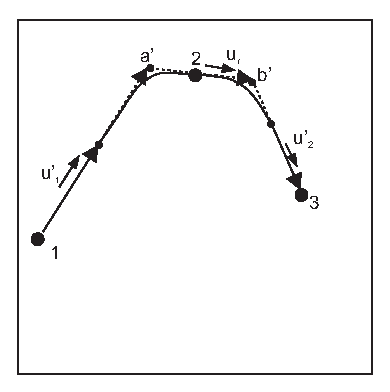
\includegraphics{figures/connetti3esatto}
        \caption{\DIFaddFL{Exact trajectory connecting three different frames by using the intermediate poses $(a')$ and $(b')$. The strategy adopted is described in \ref{subsec:connetti3esatto}.}}
        \label{fig:connetti3esatto}
    \end{minipage}
    \hfill
    \begin{minipage}[t]{0.49\textwidth}
        \centering
        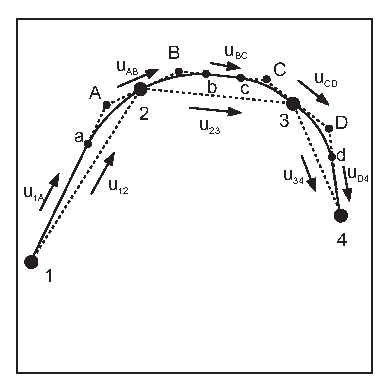
\includegraphics[width=6cm]{figures/connetti4esatto.eps}
        \caption{\DIFaddFL{Exact trajectory connecting four different frames by using the intermediate poses $(A)$, $(B)$, $(C)$ and $(D)$. The strategy adopted is described in \ref{subsec:connetti_esatto_general}}}
        \label{fig:legnani_general_method}
    \end{minipage}
\end{figure}

%DIF >  Unit sphere representation of approx/exact Legnani
\begin{figure}[tbp]
    \begin{minipage}[t]{0.49\textwidth}
        \centering
        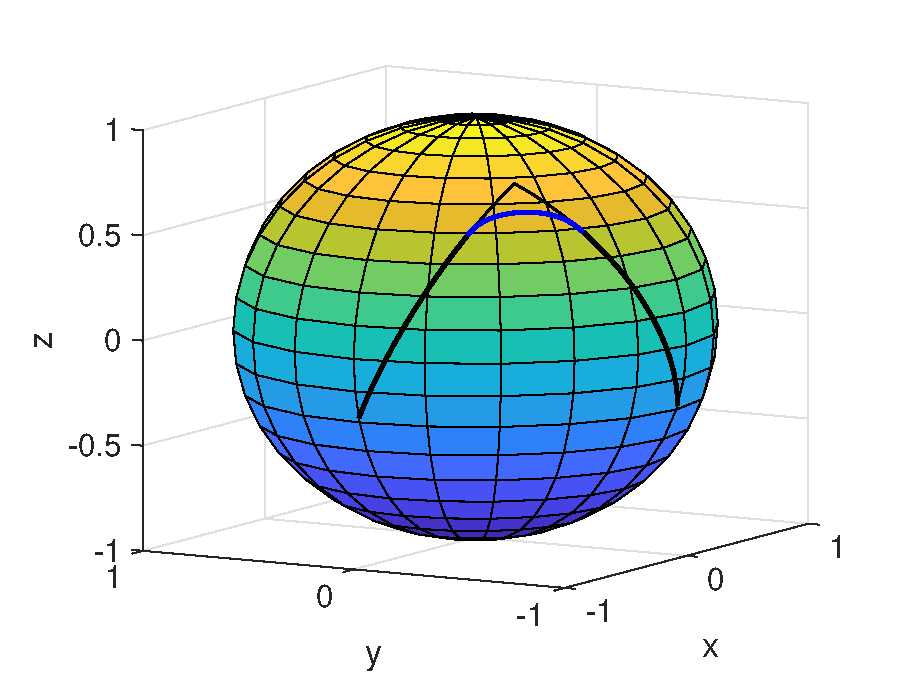
\includegraphics[width=0.95\textwidth]{figures/sfera1a}
        \caption{\DIFaddFL{Representation on the unitary sphere of the approximate algorithm (see also Fig. \ref{fig:connetti3b}).}}
        \label{fig:sfera1}
    \end{minipage}
    \hfill
    \begin{minipage}[t]{0.49\textwidth}
        \centering
        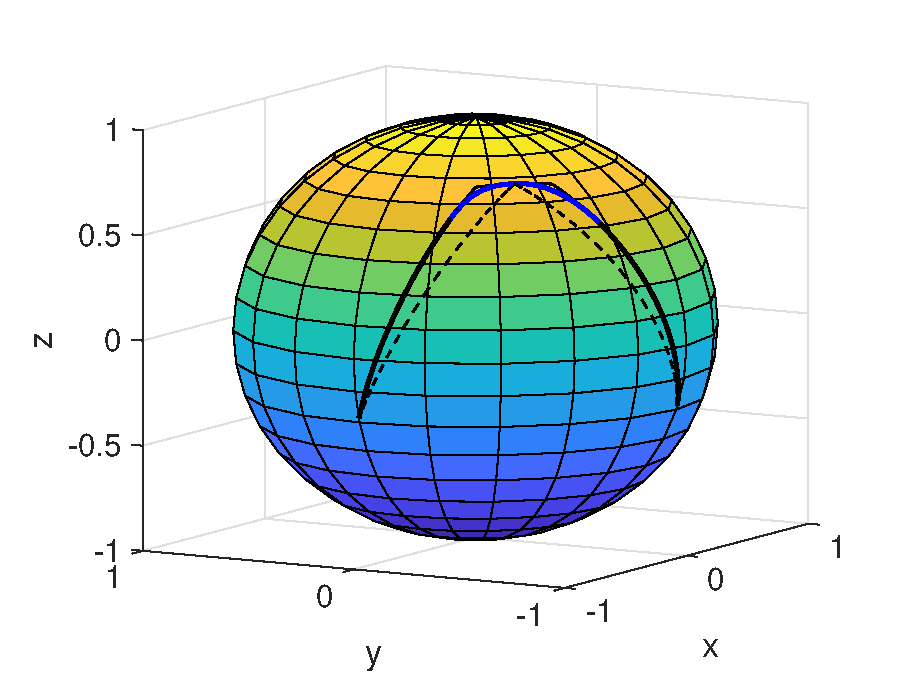
\includegraphics[width=0.95\textwidth]{figures/sfera2a}
        \caption{\DIFaddFL{Representation on the unitary sphere of the exact algorithm (see also Fig. \ref{fig:connetti3esatto}).}}
        \label{fig:sfera2}
    \end{minipage}  
\end{figure}

%DIF >  Numerical example of 3 quat interp: Legnani exact (q and w)
\begin{figure}[tbp]
    \begin{minipage}[t]{0.49\textwidth}
        \centering
        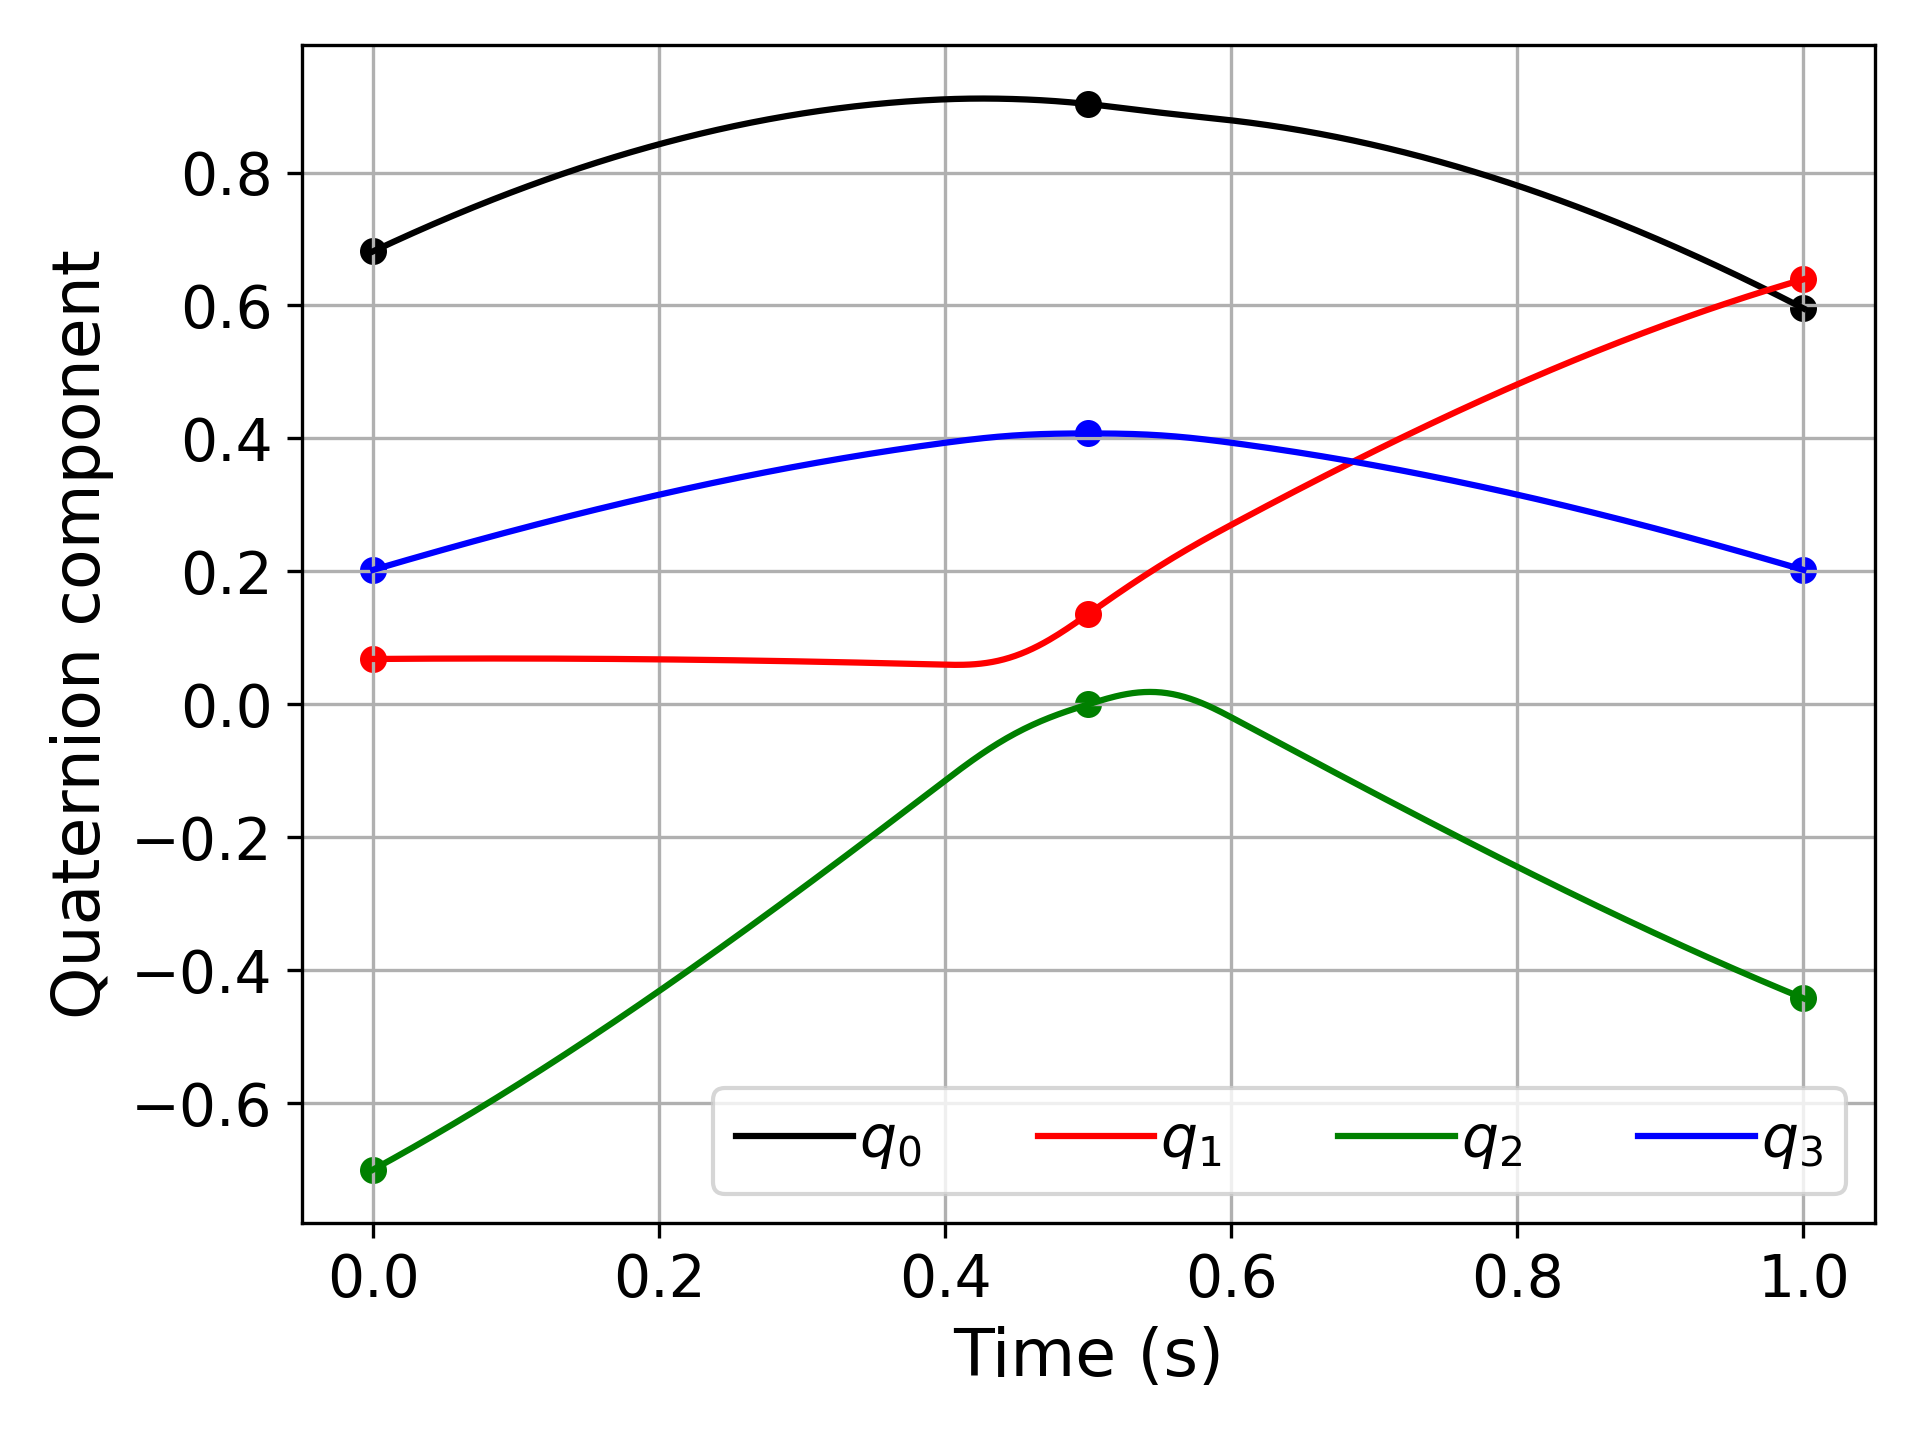
\includegraphics[width=6.5cm]{figures/legnani_exact_compo.png}
        \caption{\DIFaddFL{Numerical example of a trajectory connecting two poses and passing exactly through an intermediate pose (quaternion components versus time). The strategy adopted is described in \ref{subsec:connetti3esatto}.}}
        \label{fig:q3_legnani_exact}
    \end{minipage}
    \hfill
    \begin{minipage}[t]{0.49\textwidth}
        \centering
        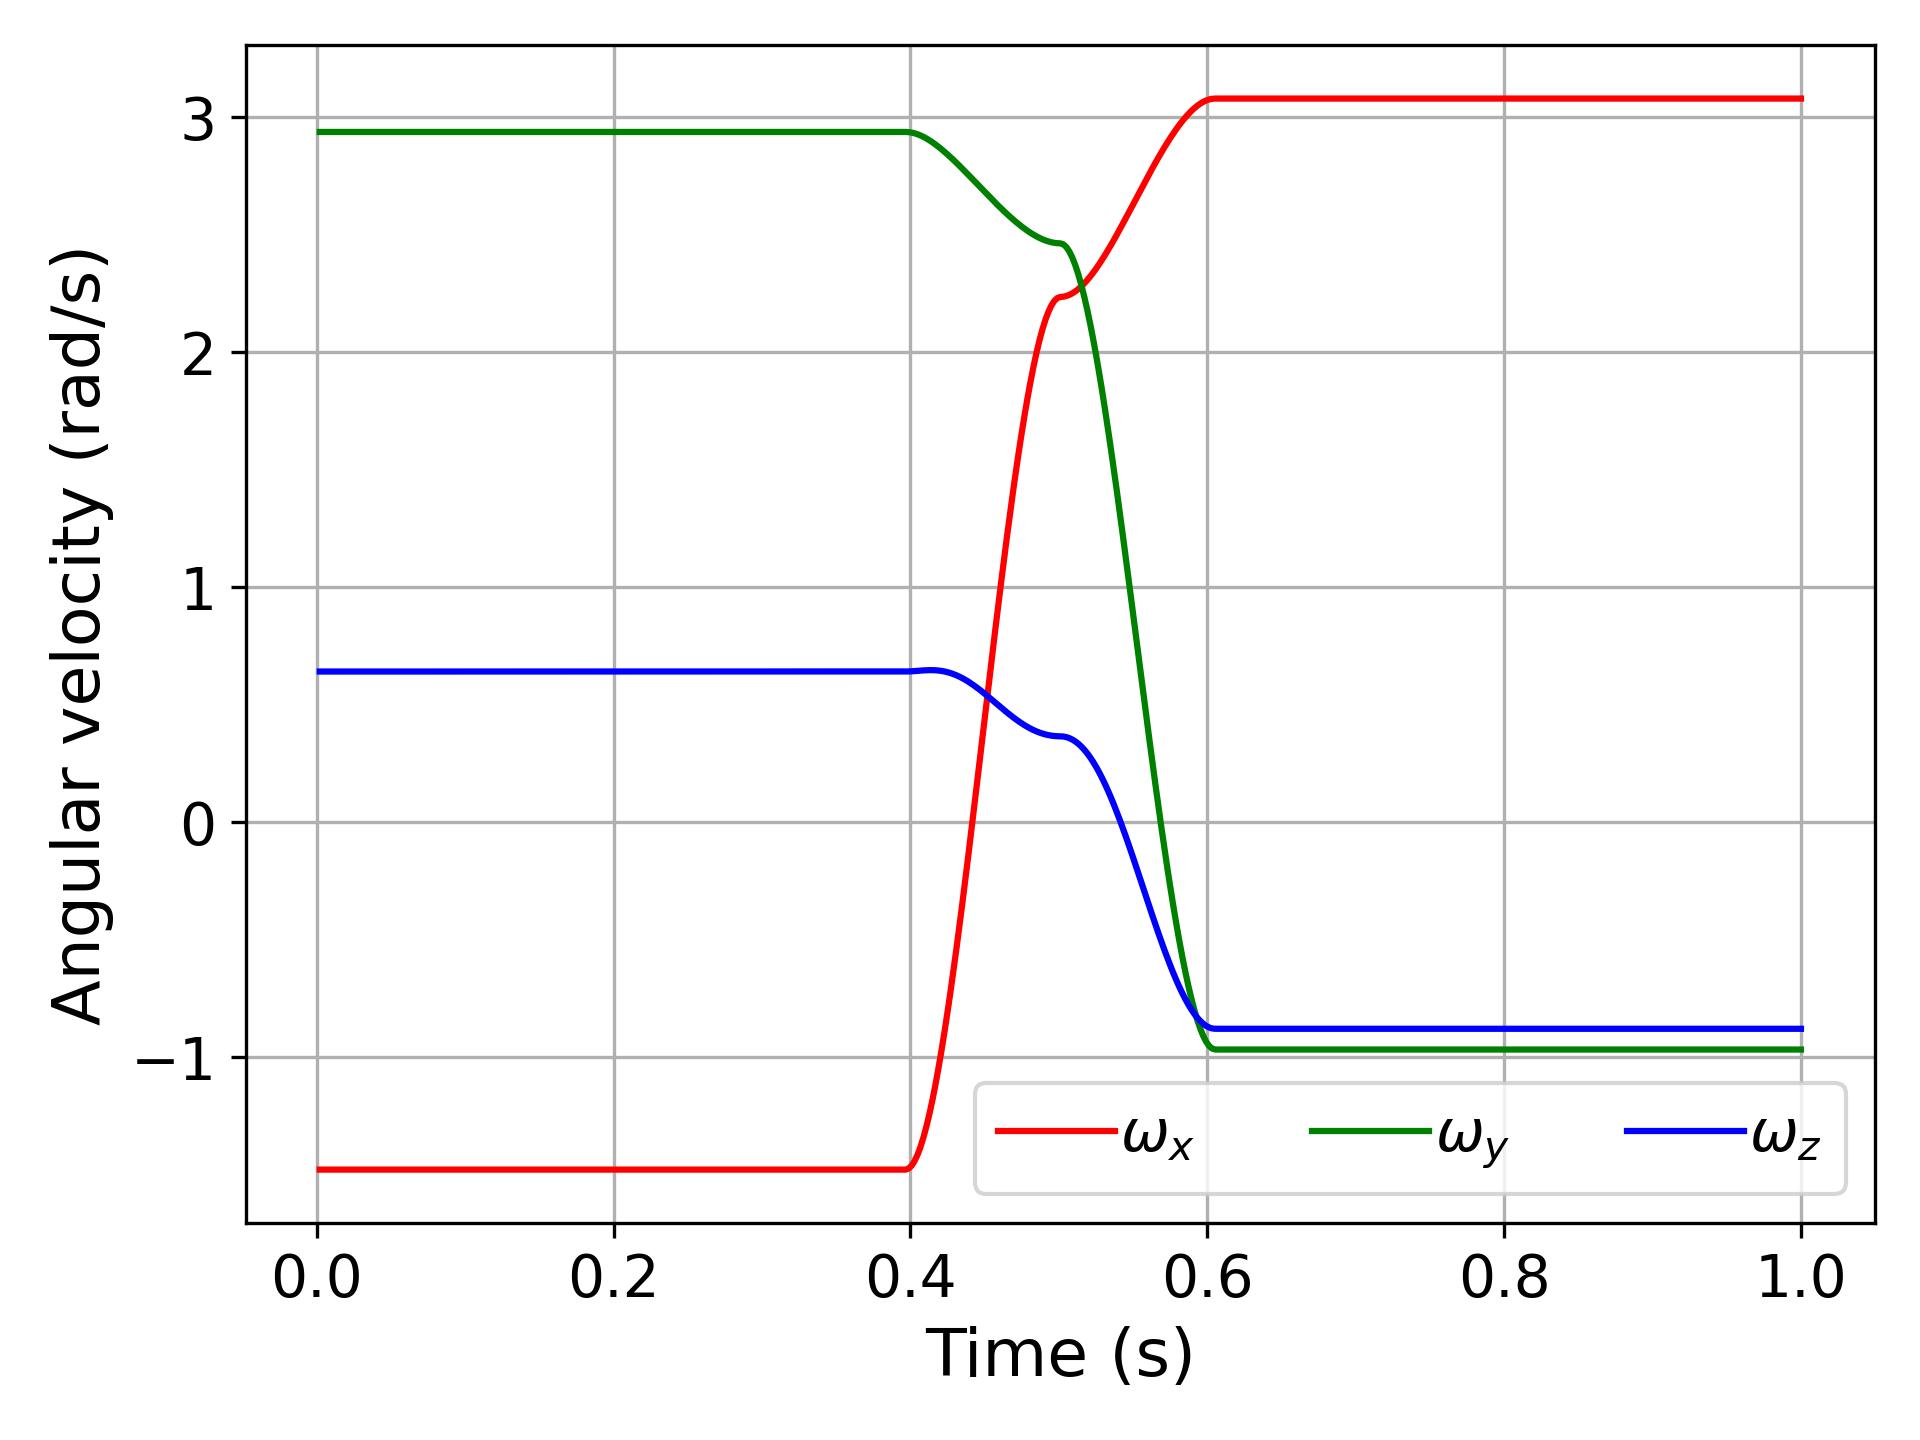
\includegraphics[width=6.5cm]{figures/legnani_exact_vel.png}
        \caption{\DIFaddFL{Angular velocity of interpolation method shown in Fig. \ref{fig:q3_legnani_exact}.}}
        \label{fig:q3_legnani_exact_velocity}
    \end{minipage}
\end{figure}

\subsection{\DIFadd{Assigning predefined velocity at the assigned poses}}
\DIFadd{The proposed algorithm generates 3D orientation trajectories connecting the assigned poses. The angular velocity profile can be easily adjusted using the following guidelines which permit to assign exact angular velocity values (modulus and direction) in the initial, intermediate and final points.}\\
\DIFadd{To assign the direction of the angular velocity it is possible to freely assign the orientation vectors used to generate the trajectory near the points (e.g. $\vect{u}_r$ in Figure \ref{fig:connetti3esatto}, and $\vect{u}_{AB}$ and $\vect{u}_{CD}$ in Figure \ref{fig:legnani_general_method}), in fact the adoption of Eq. \ref{eq:Ur} is a suggestion that generally smooth the trajectory but it is not mandatory.}\\
\DIFadd{To assign the desired modulus of the angular velocity it sufficient to apply eq. \ref{eq:deltaT} using a suitable variable value of $||\omega||$ along the trajectory. 
At first the whole trajectory is considered to evaluate the total rotation around the trajectory $\overline{\varphi}=\sum \varphi_i$. Then the desired law of variation of $\varphi$ with respect to the time is chosen ($0\leq \varphi \leq \overline{\varphi}$) respecting the desired velocity in the points of interest. This procedure permits to assign the desired value of $||\omega_i||$ for each time interval.
}

\DIFaddend %-------------------------------------------------------------------------------
\section{Numerical examples}
\label{sec:numerical_examples}
In this section we present \DIFaddbegin \DIFadd{some }\DIFaddend numerical examples of rotation interpolation, followed by some \DIFaddbegin \DIFadd{illustrated }\DIFaddend applications.

First of all, we can quantitatively compare the presented interpolation method with other common algorithms available in literature (refer to \ref{app:otherinterpolations} for further information). To this purpose, we assign some rotation \DIFaddbegin \DIFadd{key }\DIFaddend frames and observe the four quaternion component trends together with the corresponding angular velocity components, both of which with respect to \DIFdelbegin \DIFdel{the interpolation parameter $s \in [0, 1]$}\DIFdelend \DIFaddbegin \DIFadd{time $t \in [0, 1]$}\DIFaddend . In particular, we compare the SLERP \cite{shoemake1985animating} method, a \DIFdelbegin \DIFdel{2nd-order }\DIFdelend \DIFaddbegin \DIFadd{2\textsuperscript{nd}-order }\DIFaddend quaternion B-Spline method (based on \cite{kim1995ac}), the SQUAD method (based on \cite{Shoemake1987QuaternionCA} implementation) and the proposed method. We observe that:

\begin{itemize}
    \item SLERP passes though all the imposed frames without overshoots and minimizes the angular path. Velocity is piecewise constant but manifests abrupt discontinuities at curve joints \DIFaddbegin \DIFadd{(step variations); consequently, angular acceleration locally presents infinite values}\DIFaddend . See Fig. \ref{fig:chrono_spline1_compo} and Fig. \ref{fig:chrono_spline1_vel}.
    \item \DIFdelbegin \DIFdel{2nd-order }\DIFdelend \DIFaddbegin \DIFadd{2\textsuperscript{nd}-order }\DIFaddend quaternion B-Spline is very smooth, but \DIFdelbegin \DIFdel{passes quite far from }\DIFdelend \DIFaddbegin \DIFadd{does not exactly reach }\DIFaddend the intermediate imposed frames. Velocity is continuous \DIFaddbegin \DIFadd{and mainly constituted by linear tracts}\DIFaddend , but presents drastically rapid changes at curve joints\DIFaddbegin \DIFadd{; consequently, angular acceleration will locally be very high}\DIFaddend . See Fig. \ref{fig:chrono_spline2_compo} and Fig. \ref{fig:chrono_spline2_vel}.
    \item SQUAD exactly interpolates all the given poses \DIFdelbegin \DIFdel{but slightly increases the }\DIFdelend \DIFaddbegin \DIFadd{at the cost of a slight increase of the }\DIFaddend angular path. Velocity is continuous and \DIFdelbegin \DIFdel{mostly }\DIFdelend smooth but it manifests a continuously variable and bouncy trend. See Fig. \ref{fig:chrono_squad_compo} and Fig. \ref{fig:chrono_squad_vel}.
    \item The proposed \DIFdelbegin \DIFdel{extended }\DIFdelend method produces a smooth trajectory, exactly passing through all the given poses with \DIFdelbegin \DIFdel{moderate oscillations about the minimal path (with respect to the ``optimal'' SLERP ); it presents, however, }\DIFdelend \DIFaddbegin \DIFadd{modest deviation from the minimal SLERP path and }\DIFaddend slight overshoots at curve joints. \DIFdelbegin \DIFdel{Velocity }\DIFdelend \DIFaddbegin \DIFadd{As for SLERP, velocity }\DIFaddend is preserved constant through the in-between interpolation tracts, \DIFdelbegin \DIFdel{while }\DIFdelend \DIFaddbegin \DIFadd{but with the advantage of smooth connections }\DIFaddend at curve joints\DIFdelbegin \DIFdel{is smoothly connected with the next segment. }\DIFdelend \DIFaddbegin \DIFadd{. The transitions can be arbitrarily adapted to fulfil specific local constraints. }\DIFaddend See Fig. \ref{fig:legnani_eqspaced_compo} and \DIFaddbegin \DIFadd{Fig. }\DIFaddend \ref{fig:legnani_eqspaced_vel}.
\end{itemize}

To better visualize the achieved results in rotation interpolation, we present \DIFdelbegin \DIFdel{snapshots from }\DIFdelend \DIFaddbegin \DIFadd{some snapshots of a }\DIFaddend 3D \DIFdelbegin \DIFdel{animations generated with a }\DIFdelend \DIFaddbegin \DIFadd{simulation as well. The task was performed by leveraging an open-source }\DIFaddend multibody simulation engine (Chrono::Engine \cite{tasora2015chrono})\DIFdelbegin \DIFdel{where we implementedour algorithm. 
}\DIFdelend \DIFaddbegin \DIFadd{, in which the discussed algorithms were implemented. 
}

\DIFaddend Fig. \ref{fig:strobo_trail} shows a free body subject to the spatial and rotational interpolation of four key poses (blue). The red/green/blue curves are integral with the X/Y/Z local axes of the moving body, while in gray we shown the stroboscopic trail of the configurations. \DIFaddbegin \DIFadd{All the poses are smoothly and exactly connected. }\DIFaddend Fig. \ref{fig:axes_trail} shows a comparison between the proposed method and SLERP; the four imposed rotation frames are the same as the previous ones (Fig. \ref{fig:strobo_trail}), but there is no spatial motion. One can observe the undesired spikes produced by SLERP by looking at the red/green/blue axes curves. \DIFdelbegin %DIFDELCMD < 

%DIFDELCMD < %%%
\DIFdel{Finally, in }\DIFdelend \DIFaddbegin \DIFadd{Finally, }\DIFaddend Fig. \ref{fig:chrono_robot} \DIFdelbegin \DIFdel{we show the }\DIFdelend \DIFaddbegin \DIFadd{shows a potential application of the proposed algorithm: the }\DIFaddend smooth interpolation of poses performed by the end-effector of an industrial robot \DIFdelbegin \DIFdel{, }\DIFdelend \DIFaddbegin \DIFadd{(}\DIFaddend namely a 6-DOF robot arm equipped with painting tools\DIFaddbegin \DIFadd{)}\DIFaddend .

% Numerical example of 6 quat interp: SLERP (q and w)
\begin{figure}[tbp]
    \begin{minipage}[t]{0.49\textwidth}
        \DIFaddbeginFL \centering
        \DIFaddendFL 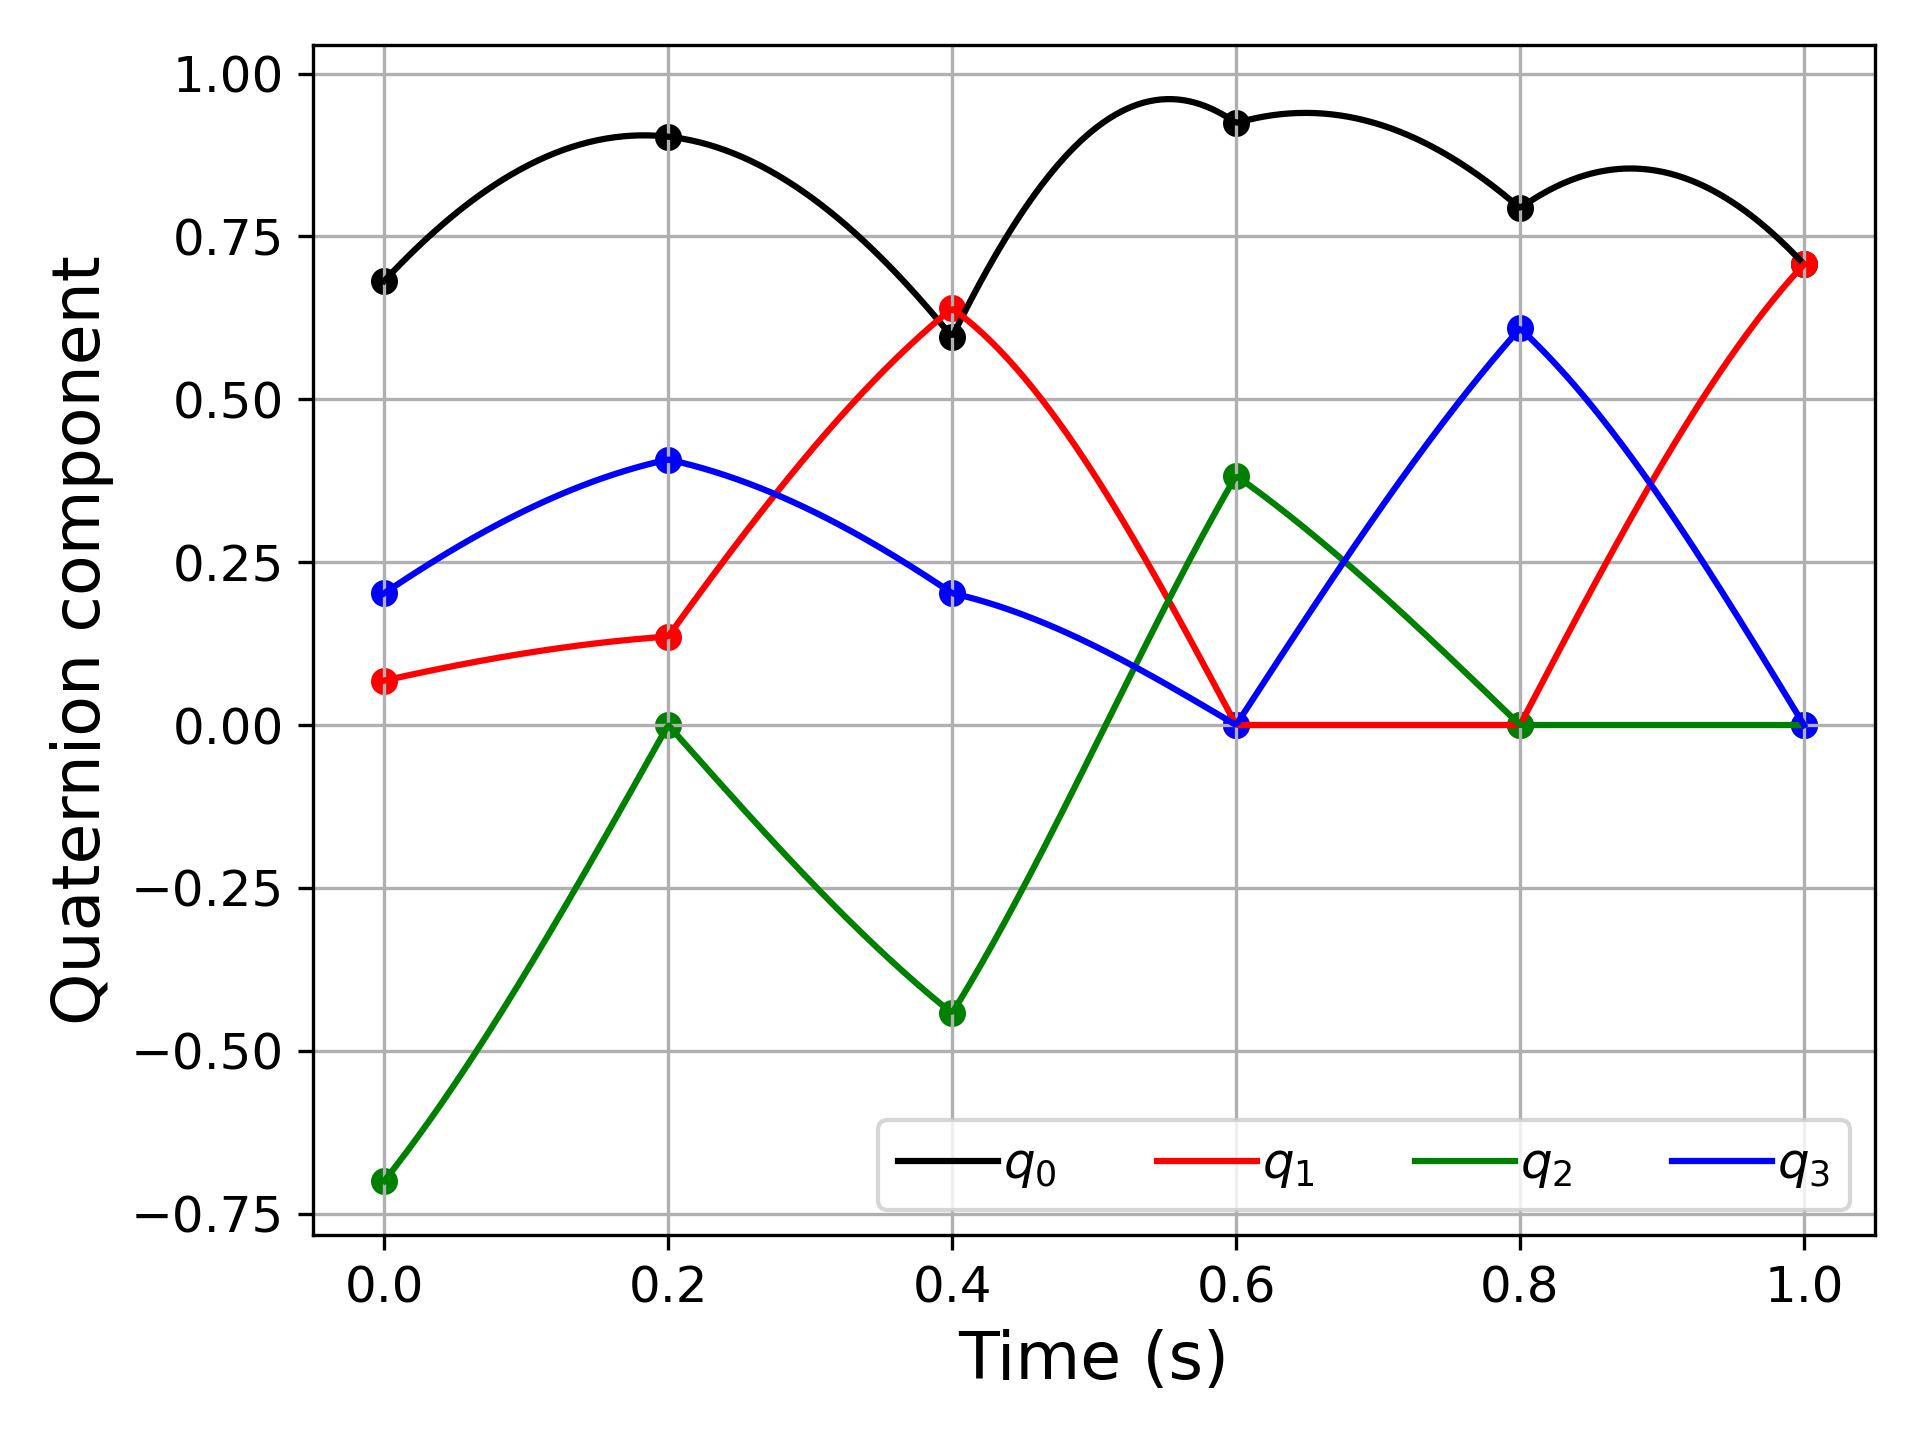
\includegraphics[width=6cm]{figures/chrono_spline1_compo.png}
        \caption{Numerical example of a trajectory connecting six poses using the SLERP interpolation method (quaternion components versus time). \DIFaddbeginFL \DIFaddFL{All the given frames are exactly reached by a non-smooth trajectory, having minimum angular length.}\DIFaddendFL }
        \label{fig:chrono_spline1_compo}
    \end{minipage}
    \hfill
    \begin{minipage}[t]{0.49\textwidth}
        \DIFaddbeginFL \centering
        \DIFaddendFL 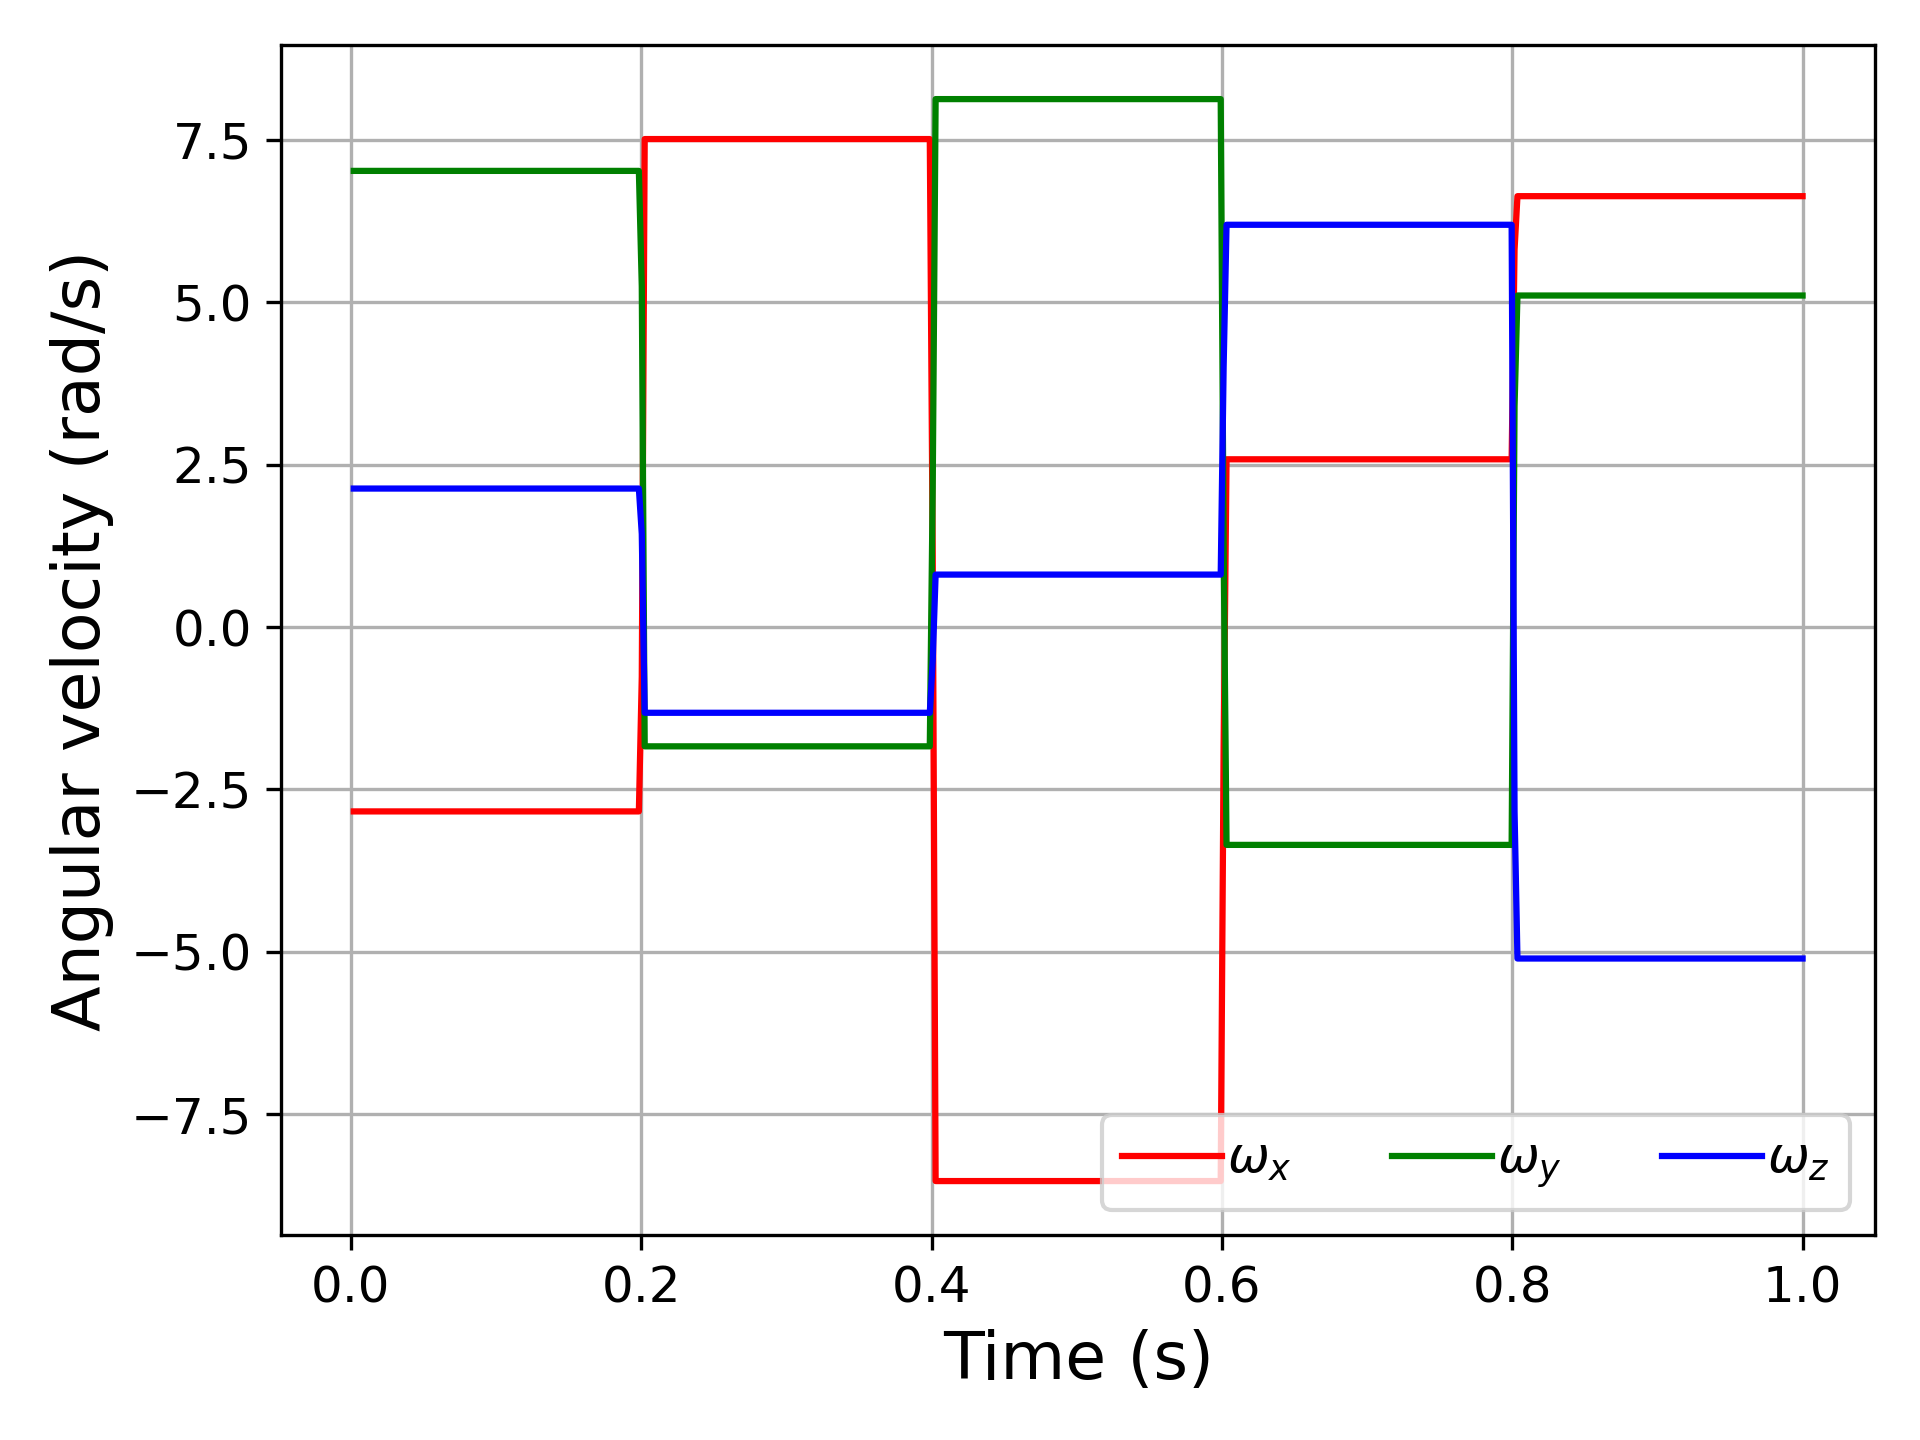
\includegraphics[width=6.5cm]{figures/chrono_spline1_vel.png}
        \caption{Angular velocity of SLERP interpolation method shown in Fig. \ref{fig:chrono_spline1_compo}\DIFaddbeginFL \DIFaddFL{. Severe discontinuities at curve joints are notable.}\DIFaddendFL }
        \label{fig:chrono_spline1_vel}
    \end{minipage}
\end{figure}

% Numerical example of 6 quat interp: BSpline2 (q and w)
\begin{figure}[tbp]
    \begin{minipage}[t]{0.49\textwidth}
        \DIFaddbeginFL \centering
        \DIFaddendFL 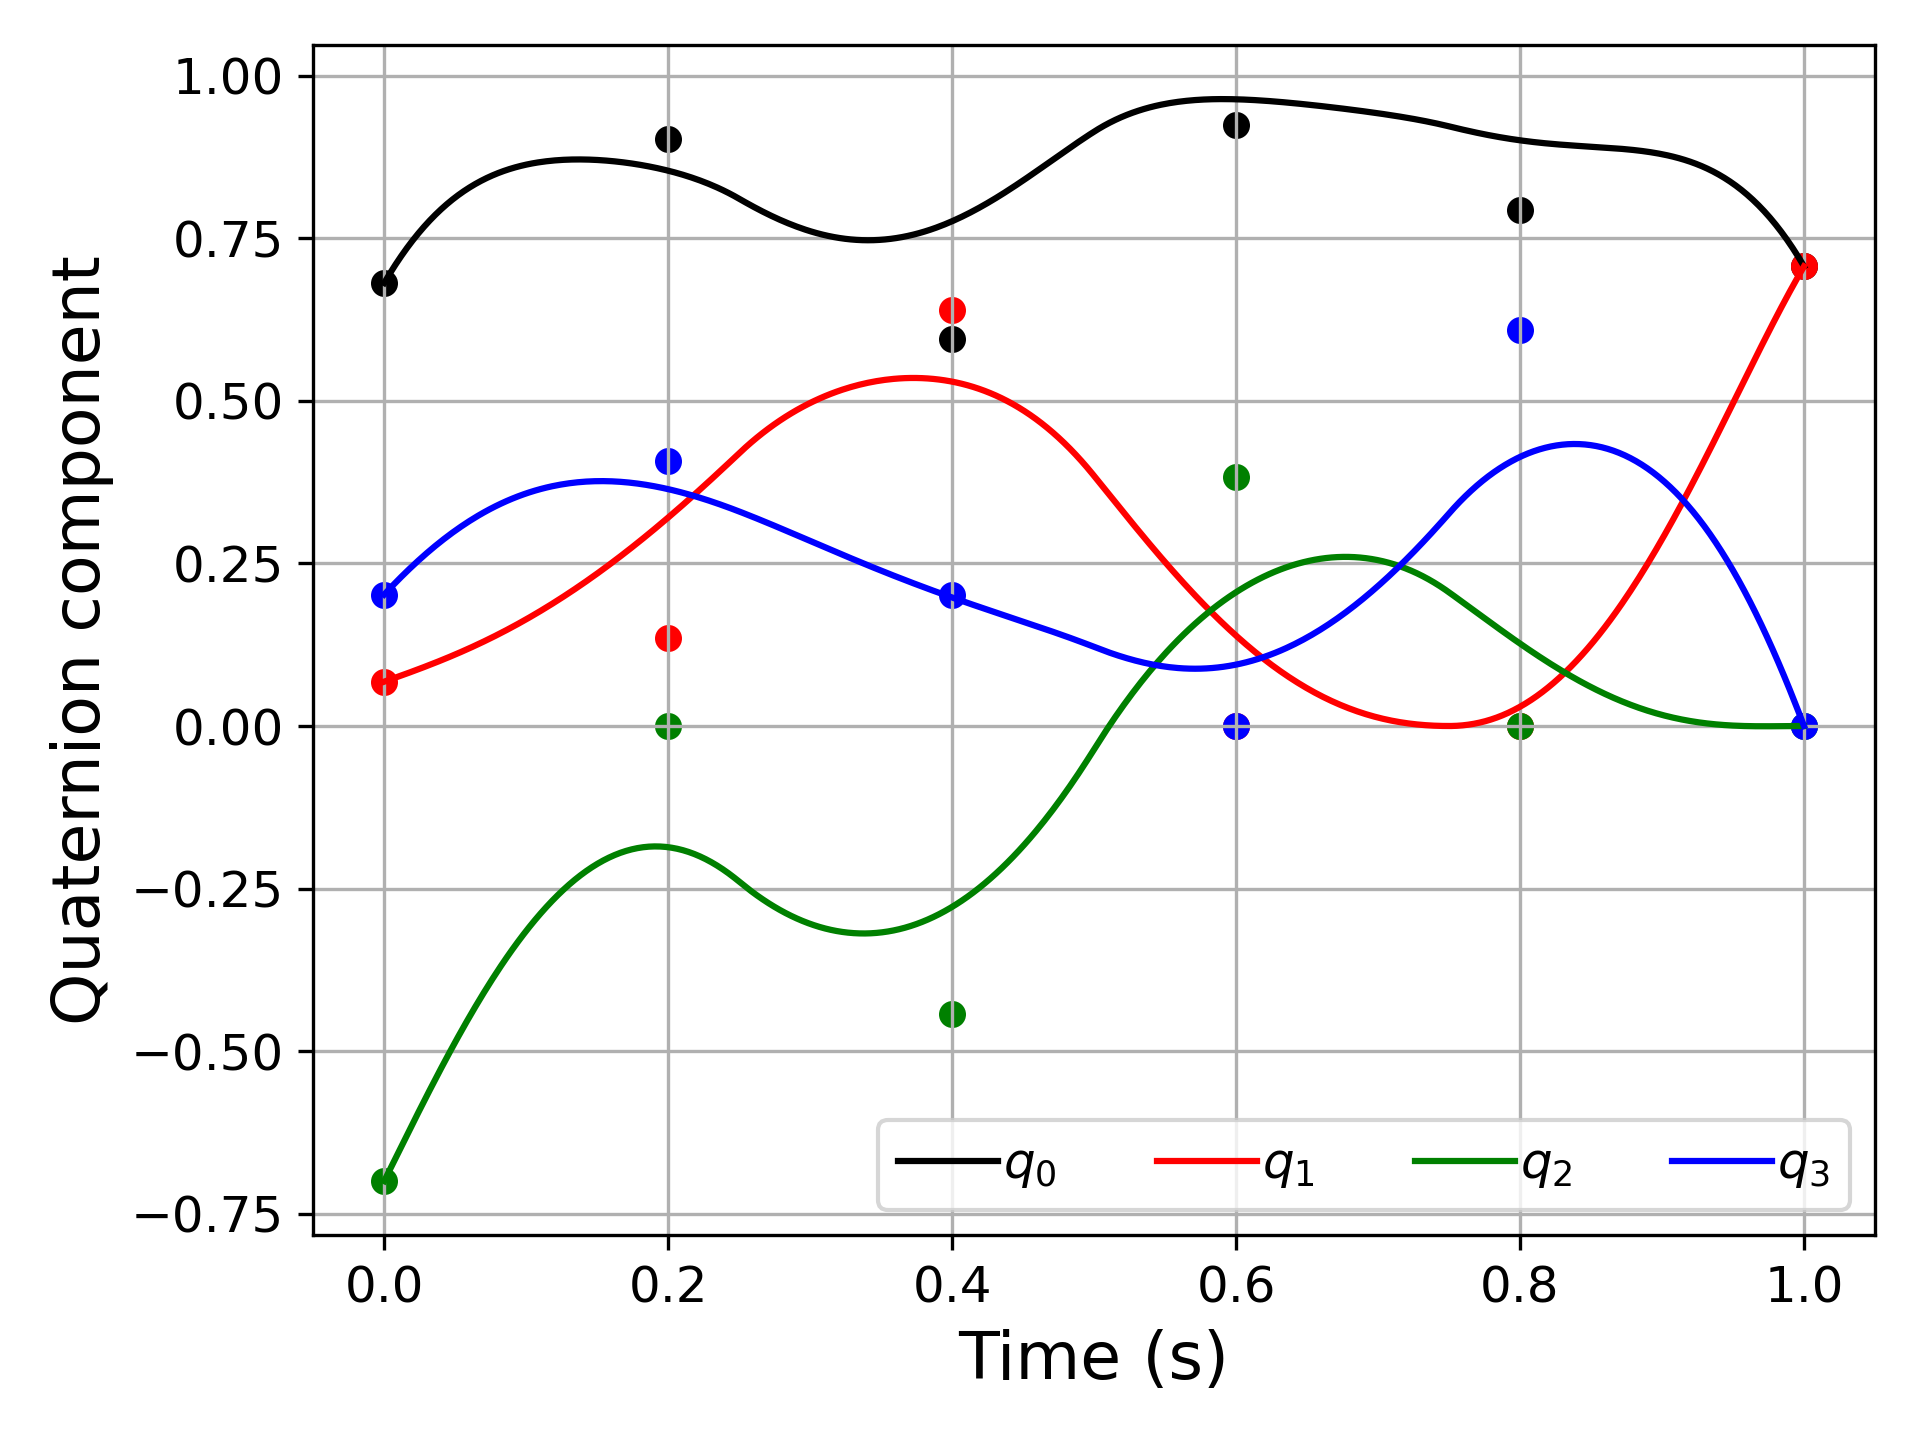
\includegraphics[width=6.5cm]{figures/chrono_spline2_compo.png}
        \caption{Numerical example of a trajectory connecting six poses using a \DIFdelbeginFL \DIFdelFL{2nd-order }\DIFdelendFL \DIFaddbeginFL \DIFaddFL{2\textsuperscript{nd}-order }\DIFaddendFL quaternion B-Spline (quaternion components versus time). \DIFaddbeginFL \DIFaddFL{Angular trajectory is very smooth, but does not exactly pass through all the given frames.}\DIFaddendFL }
        \label{fig:chrono_spline2_compo}
    \end{minipage}
    \hfill
    \begin{minipage}[t]{0.49\textwidth}
        \DIFaddbeginFL \centering
        \DIFaddendFL 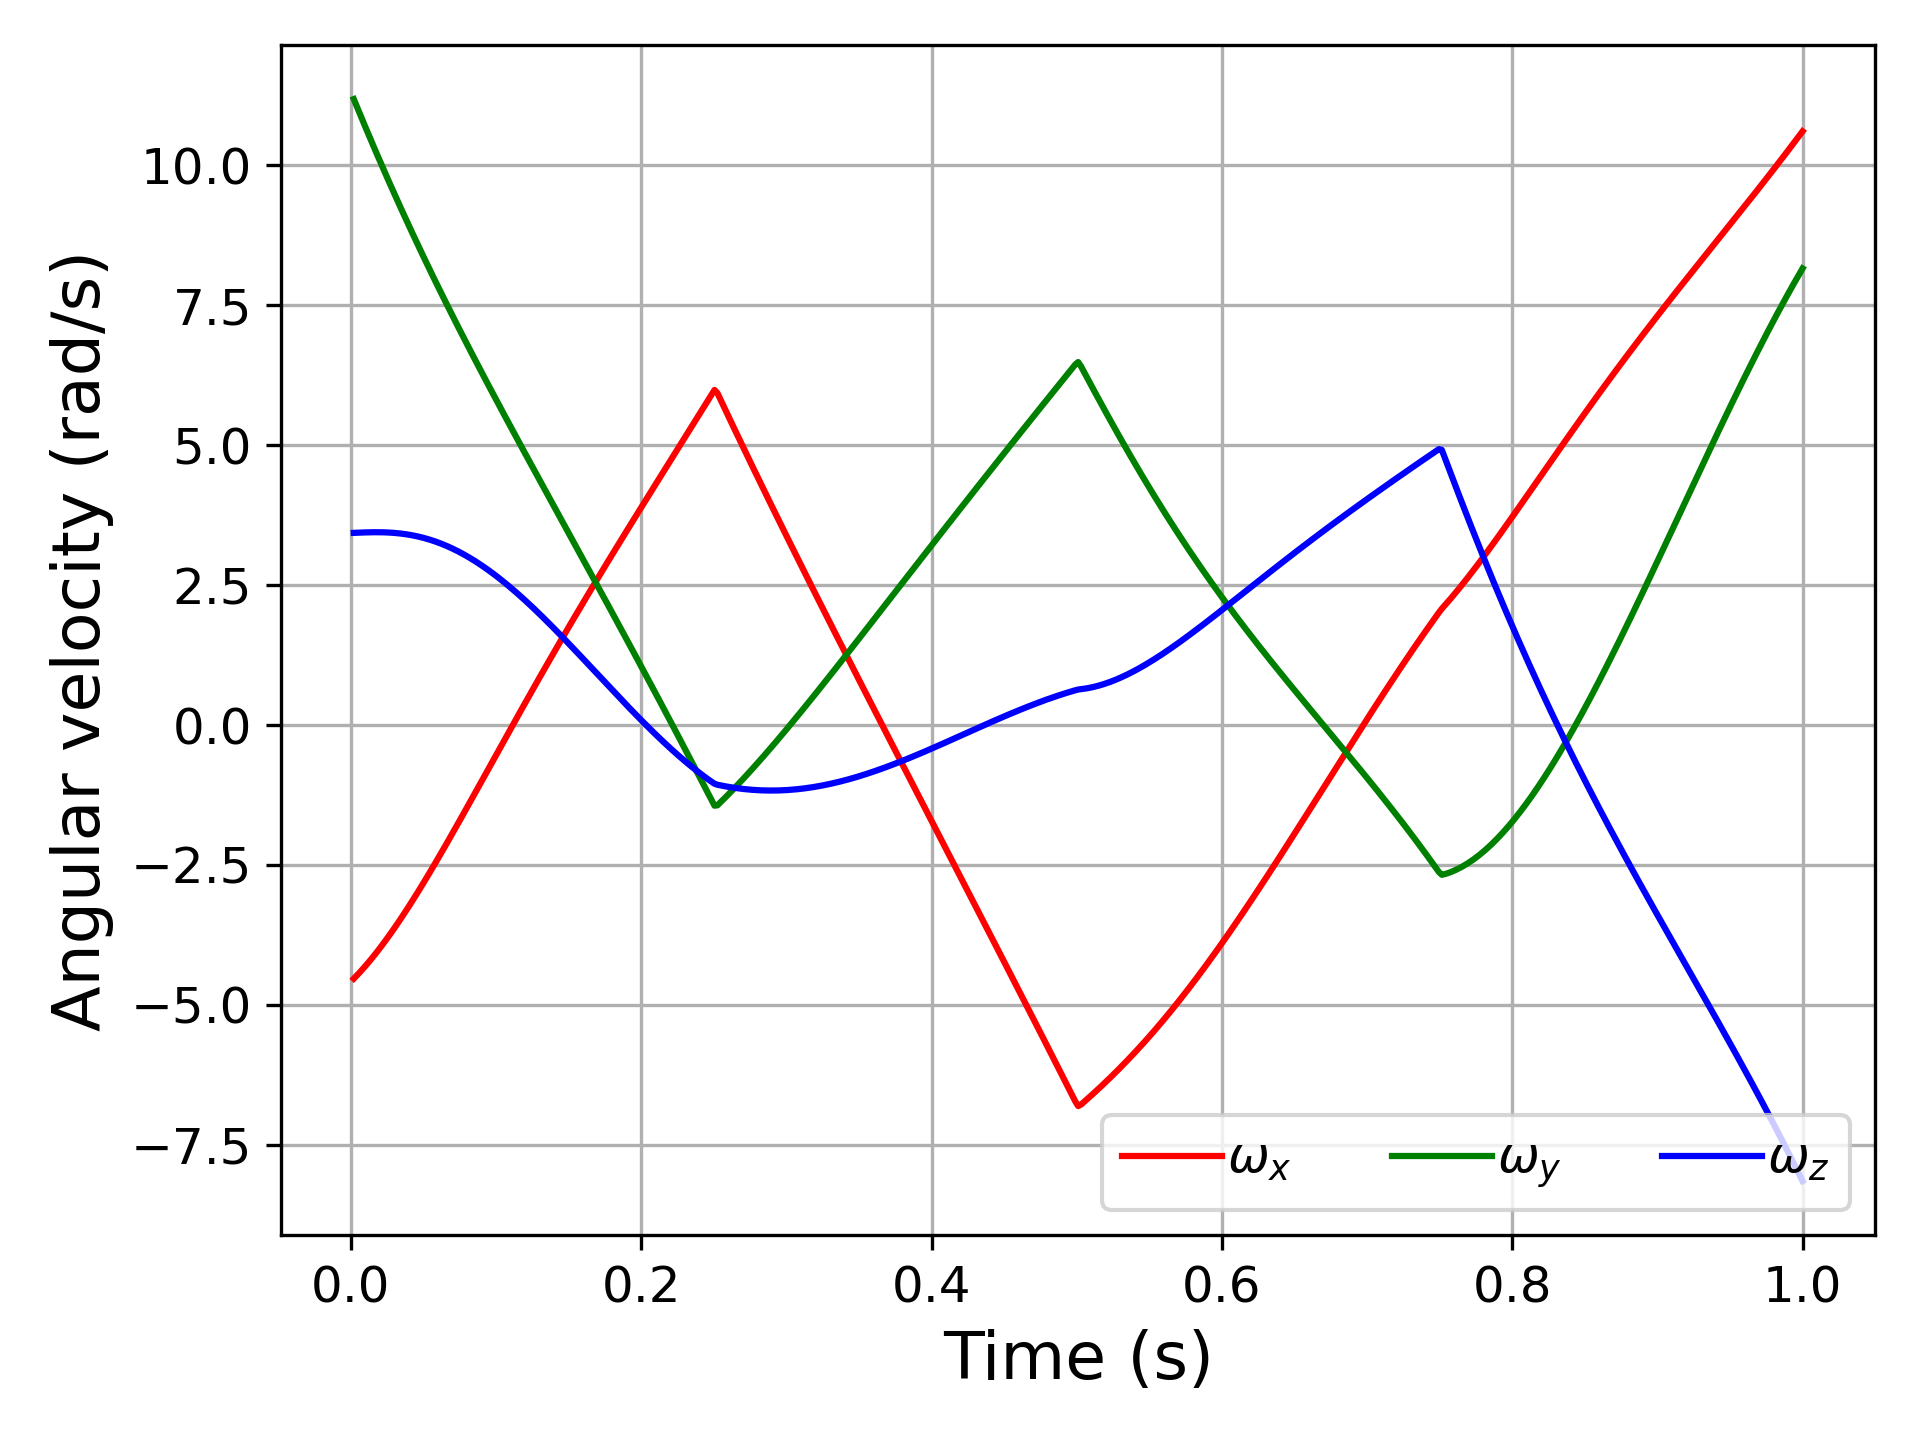
\includegraphics[width=6.5cm]{figures/chrono_spline2_vel.png}
        \caption{Angular velocity of \DIFdelbeginFL \DIFdelFL{2nd-order }\DIFdelendFL \DIFaddbeginFL \DIFaddFL{2\textsuperscript{nd}-order }\DIFaddendFL quaternion B-Spline interpolation method shown in Fig. \ref{fig:chrono_spline2_compo}. \DIFaddbeginFL \DIFaddFL{The trend is continuous, but with abrupt spikes at curve joints.}\DIFaddendFL }
        \label{fig:chrono_spline2_vel}
    \end{minipage}
\end{figure}

% Numerical example of 6 quat interp: SQUAD (q and w)
\begin{figure}[tbp]
    \begin{minipage}[t]{0.49\textwidth}
        \DIFaddbeginFL \centering
        \DIFaddendFL 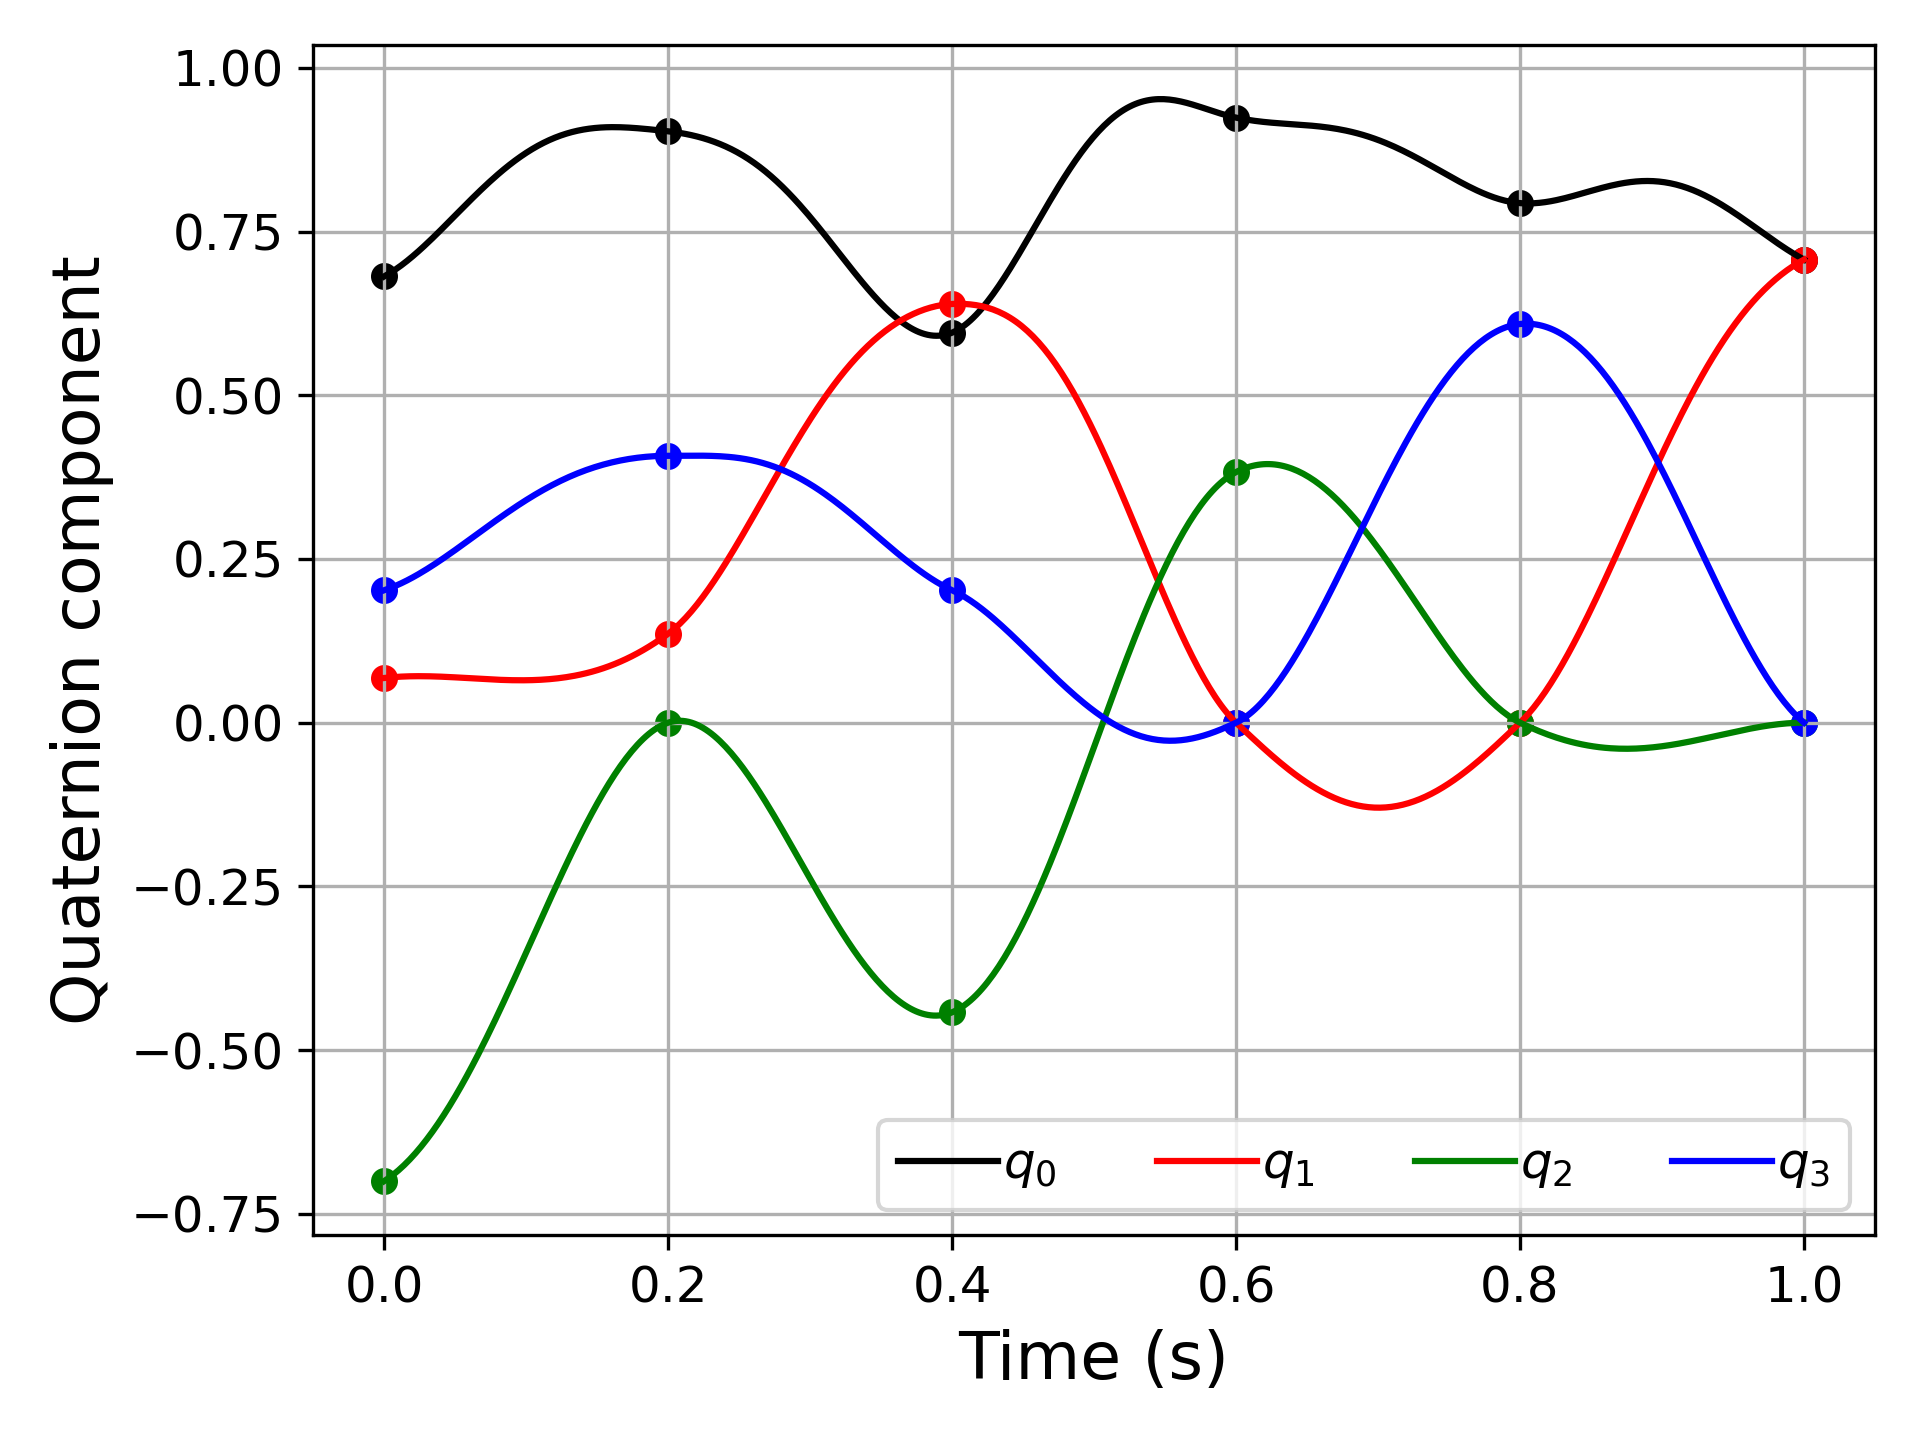
\includegraphics[width=6.5cm]{figures/chrono_squad_compo.png}
        \caption{Numerical example of a trajectory connecting six poses using the SQUAD interpolation method (quaternion components versus time). \DIFaddbeginFL \DIFaddFL{All the given frames are exactly reached by a smooth trajectory.}\DIFaddendFL }
        \label{fig:chrono_squad_compo}
    \end{minipage}
    \hfill
    \begin{minipage}[t]{0.49\textwidth}
        \DIFaddbeginFL \centering
        \DIFaddendFL 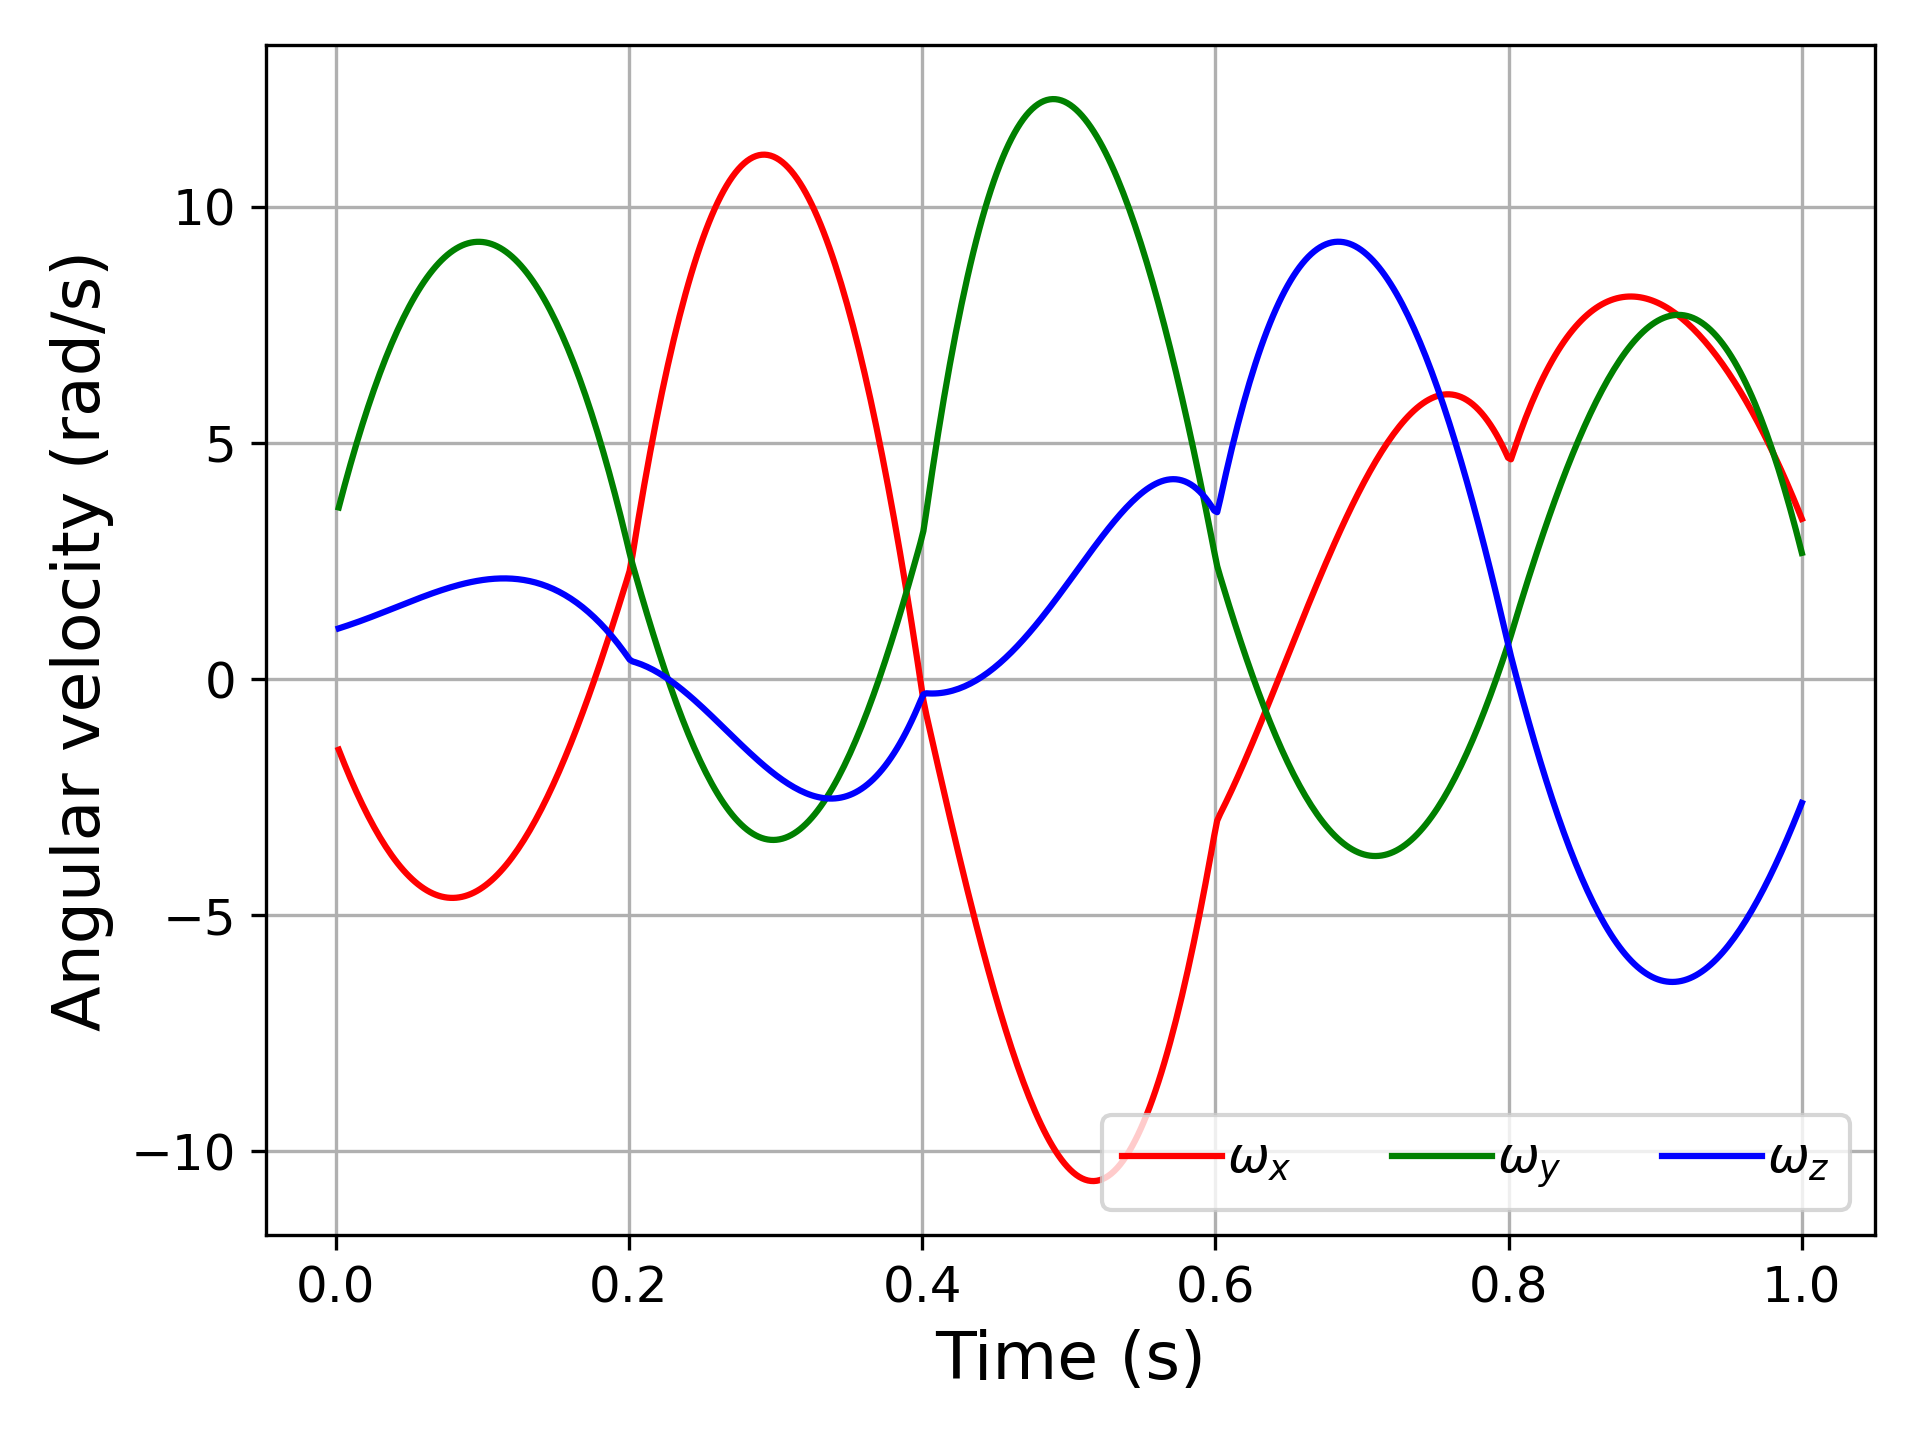
\includegraphics[width=6.5cm]{figures/chrono_squad_vel.png}
        \caption{Angular velocity of SQUAD interpolation method shown in Fig. \ref{fig:chrono_squad_compo}. \DIFaddbeginFL \DIFaddFL{The trend is continuous but highly oscillating.}\DIFaddendFL }
        \label{fig:chrono_squad_vel}
    \end{minipage}
\end{figure}

% Numerical example of 6 quat interp: Legnani exact (q and w)
\begin{figure}[tbp]
    \begin{minipage}[t]{0.49\textwidth}
        \DIFaddbeginFL \centering
        \DIFaddendFL 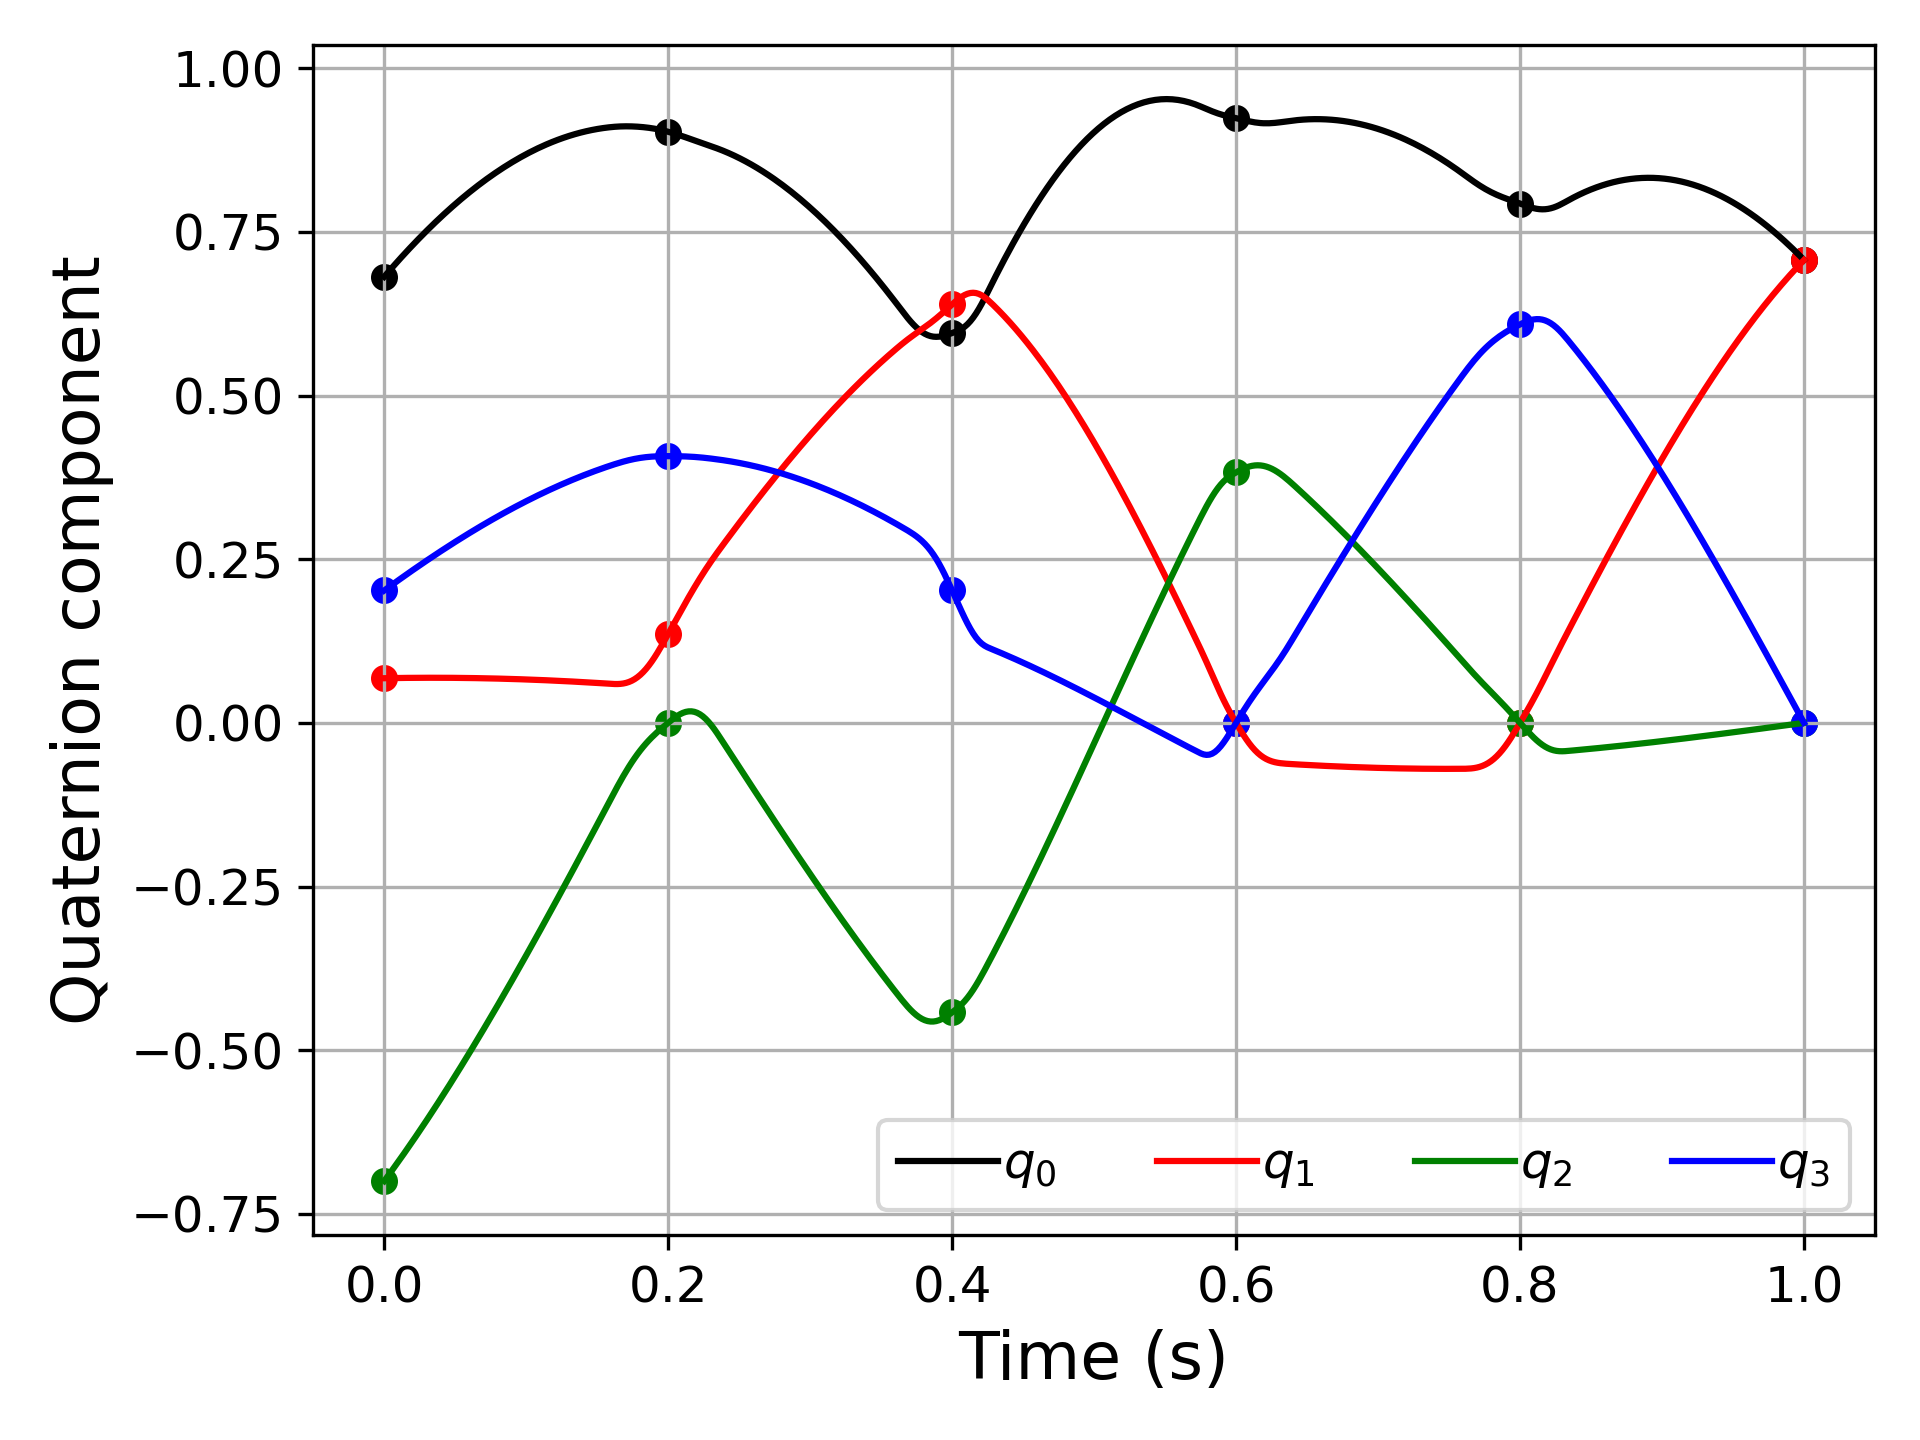
\includegraphics[width=6.5cm]{figures/legnani_eqspaced_compo.png}
        \caption{Numerical example of a trajectory connecting six poses using the proposed extended exact interpolation method (quaternion components versus time). \DIFaddbeginFL \DIFaddFL{All the given frames are exactly reached by a smooth trajectory.}\DIFaddendFL }
        \label{fig:legnani_eqspaced_compo}
    \end{minipage}
    \hfill
    \begin{minipage}[t]{0.49\textwidth}
        \DIFaddbeginFL \centering
        \DIFaddendFL 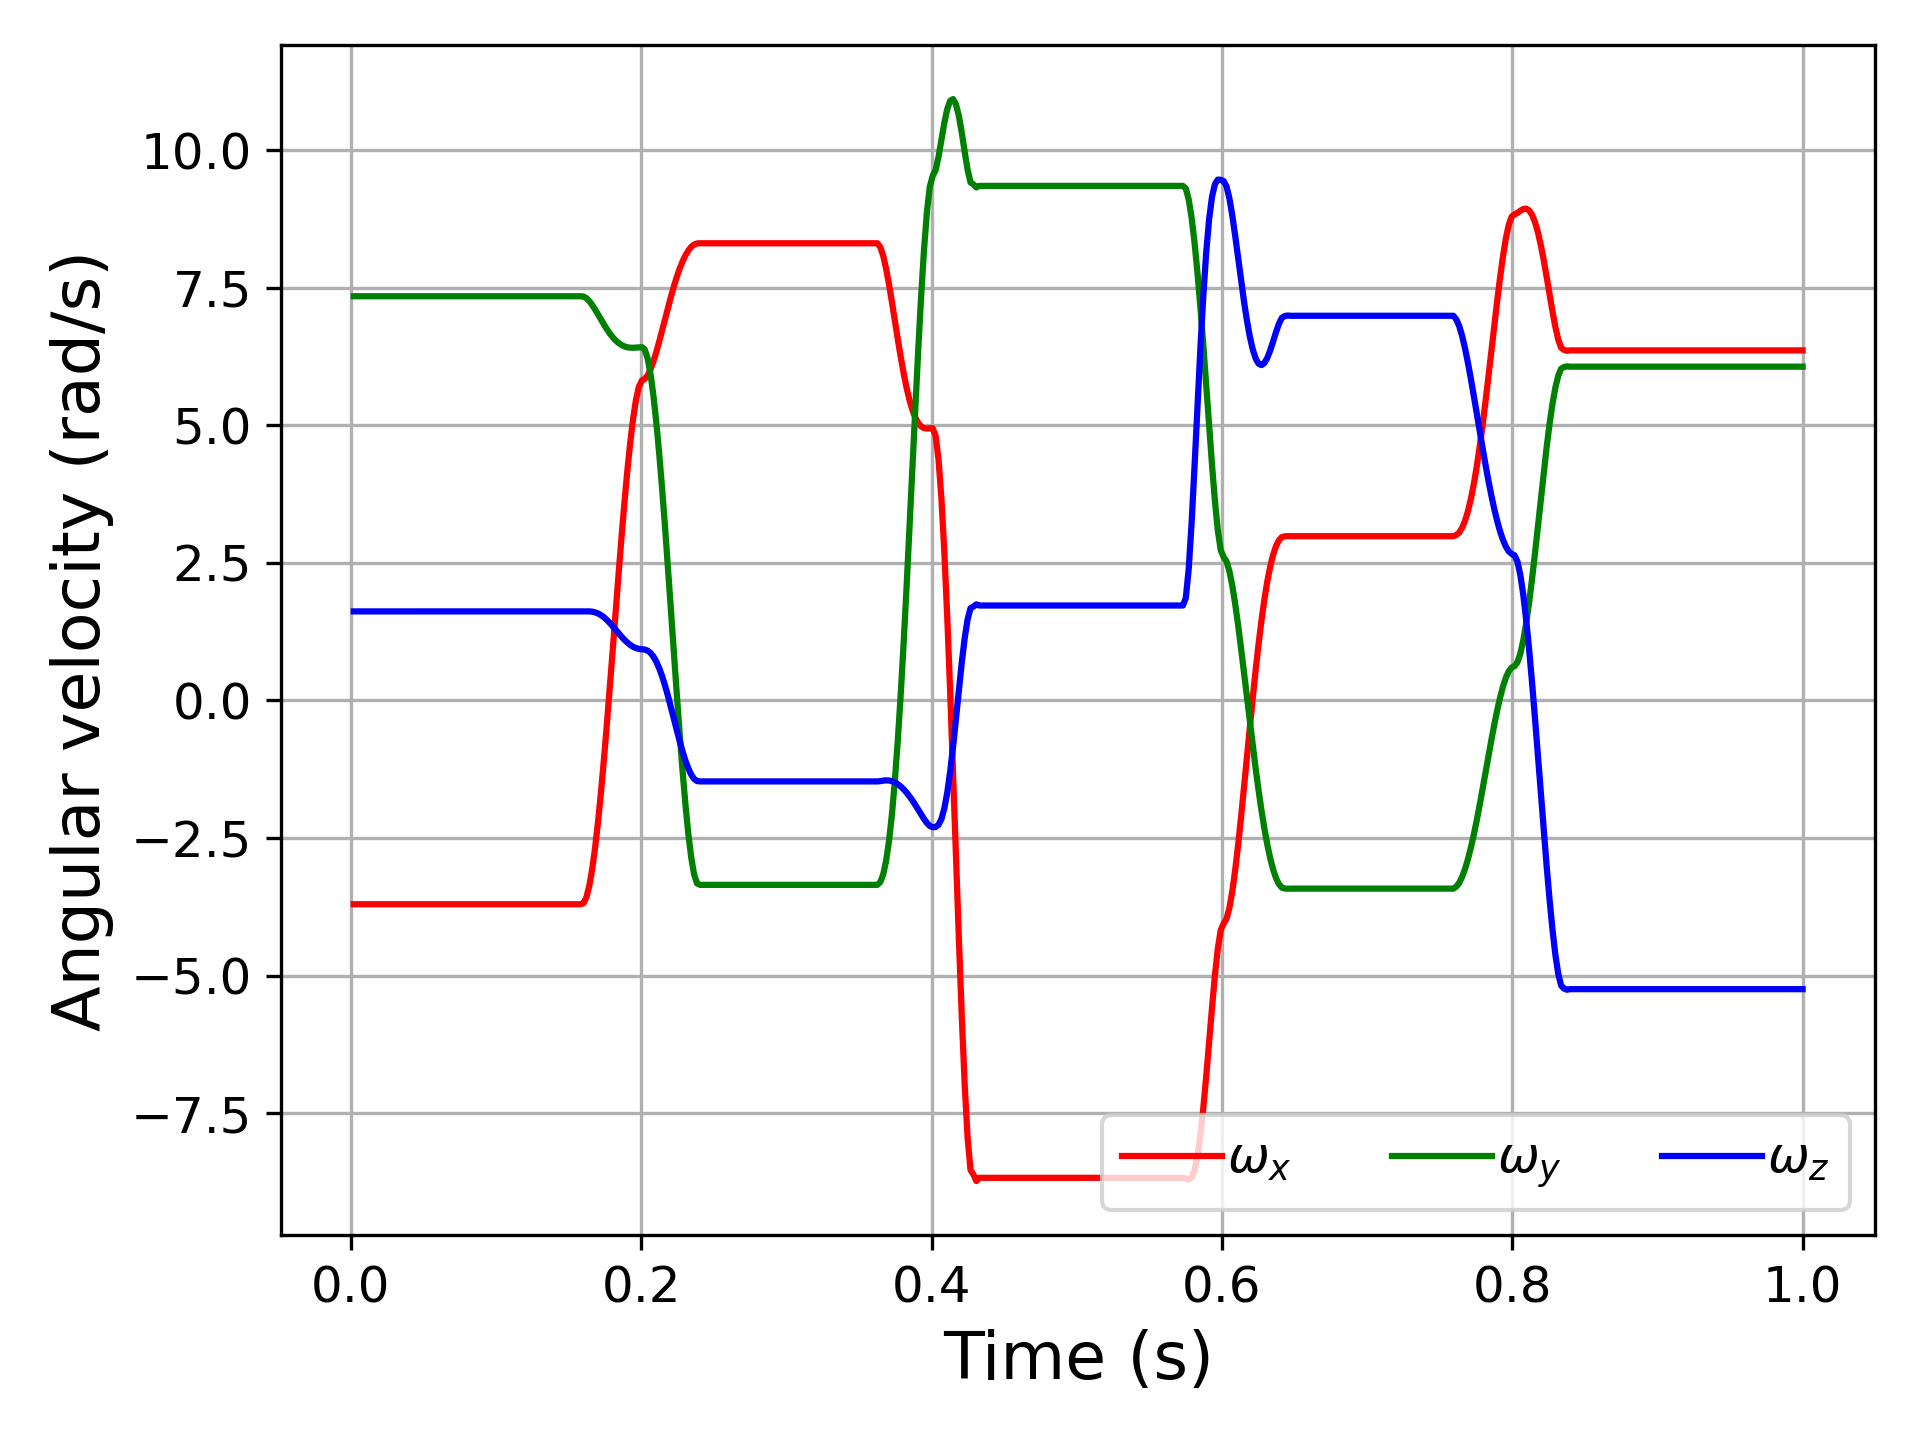
\includegraphics[width=6.5cm]{figures/legnani_eqspaced_vel.png}
        \caption{Angular velocity of the proposed extended exact interpolation method shown in Fig. \ref{fig:legnani_eqspaced_compo}. \DIFaddbeginFL \DIFaddFL{The trend remains constant over the intermediate phases and smoothly transitions from one tract to the other.}\DIFaddendFL }
        \label{fig:legnani_eqspaced_vel}
    \end{minipage}
\end{figure}

% Chrono simulation: stroboscopic trail
\begin{figure}[tbp]
    \DIFaddbeginFL \centering
    \DIFaddendFL 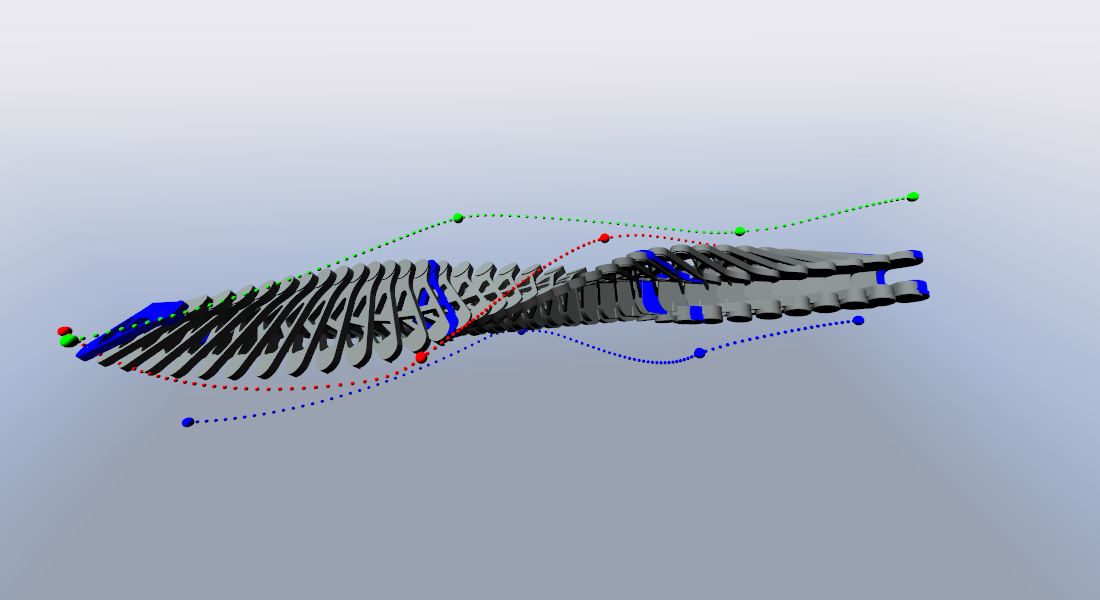
\includegraphics[trim=0 1cm 0 3cm,clip,width=0.99\textwidth]{figures/strobo_trail.PNG}
    \caption{Simulated interpolation of four poses using the proposed method in association with a spatial motion \DIFaddbeginFL \DIFaddFL{ 
\cite{tasora2015chrono} 
}\DIFaddendFL . The assigned key frames are shown in blue, while the moving body axes are represented by RGB trails (key frame passages are highlighted)\DIFdelbeginFL \DIFdelFL{ 
\cite{tasora2015chrono} 
}\DIFdelendFL . \DIFaddbeginFL \DIFaddFL{It is notable that the generated trajectory is smooth and exactly passes though all the given rotations.}\DIFaddendFL }
    \label{fig:strobo_trail}
\end{figure}

% Chrono simulation: axes trail  
\begin{figure}[tbp]
    \begin{minipage}[t]{0.49\textwidth}
        \DIFaddbeginFL \centering
        \DIFaddendFL 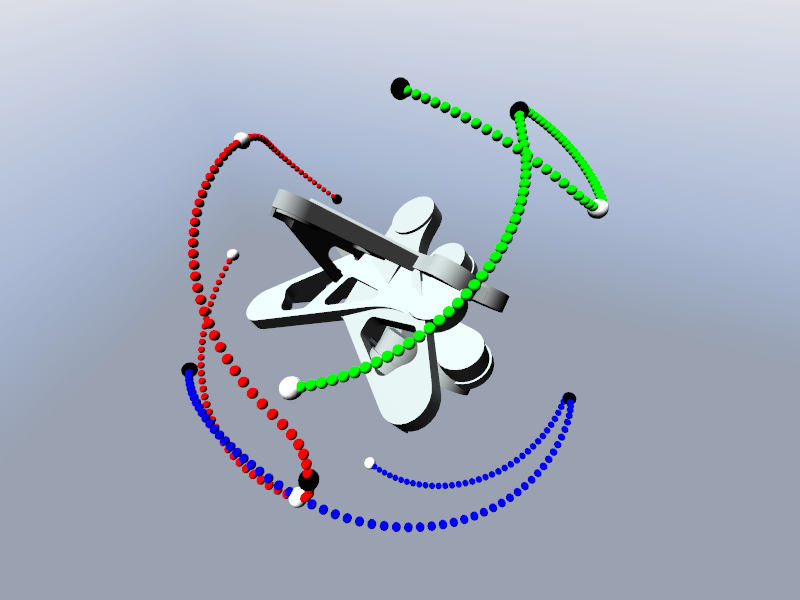
\includegraphics[width=6.5cm]{figures/axes_trail_slerp.PNG}
    \end{minipage}
    \hfill
    \begin{minipage}[t]{0.49\textwidth}
        \DIFaddbeginFL \centering
        \DIFaddendFL 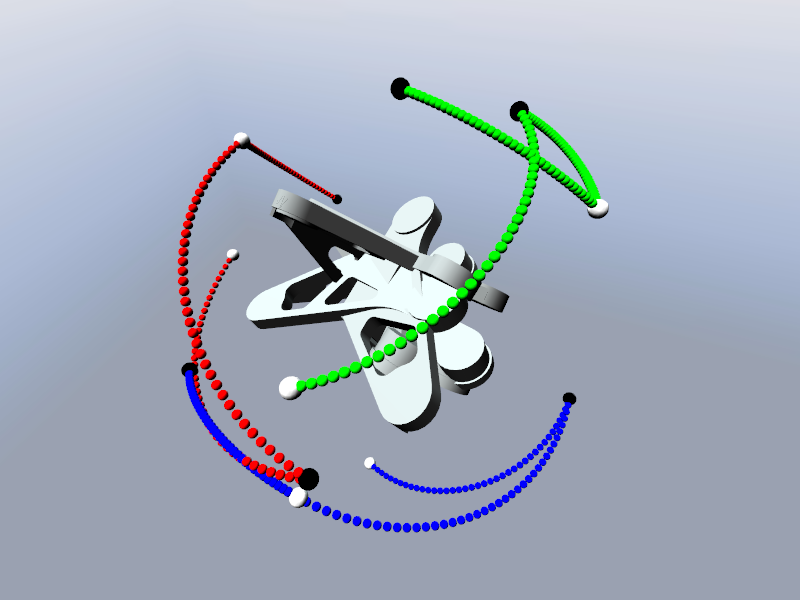
\includegraphics[width=6.5cm]{figures/axes_trail_legnani.png}
    \end{minipage}
    \caption{Simulated comparison \DIFaddbeginFL \DIFaddFL{ 
\cite{tasora2015chrono}  
}\DIFaddendFL between the proposed method (left) and SLERP (right) interpolation of the same four poses of Fig.\ref{fig:strobo_trail}, without spatial motion. The rotating body axes are represented by RGB trails and the passage through the assigned key frames is highlighted as white and black dots\DIFdelbeginFL \DIFdelFL{ 
\cite{tasora2015chrono} 
}\DIFdelendFL . It may be noted \DIFaddbeginFL \DIFaddFL{from the axes trails }\DIFaddendFL that the SLERP trajectory manifests spikes at curve joints, \DIFdelbeginFL \DIFdelFL{while our method smoothly }\DIFdelendFL \DIFaddbeginFL \DIFaddFL{therefore discontinuities in angular velocity; on the contrary, the proposed algorithm }\DIFaddendFL connects the given orientations \DIFaddbeginFL \DIFaddFL{with smooth curves}\DIFaddendFL .}
    \label{fig:axes_trail}
\end{figure}

% Chrono simulation: robot application
\begin{figure*}[tbp]
	\centering
    \subfloat[]{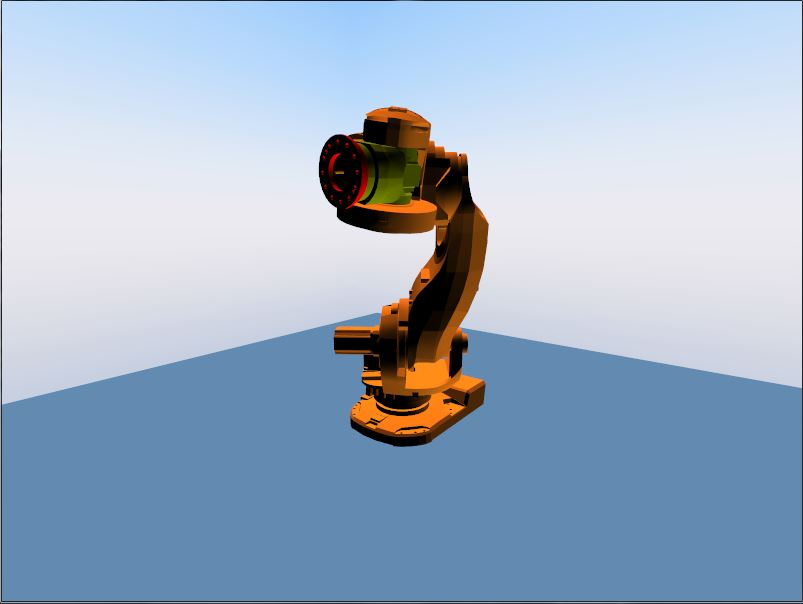
\includegraphics[width=0.45\textwidth]{figures/robot1.jpg}}
    % \hfill
    % \subfloat[]{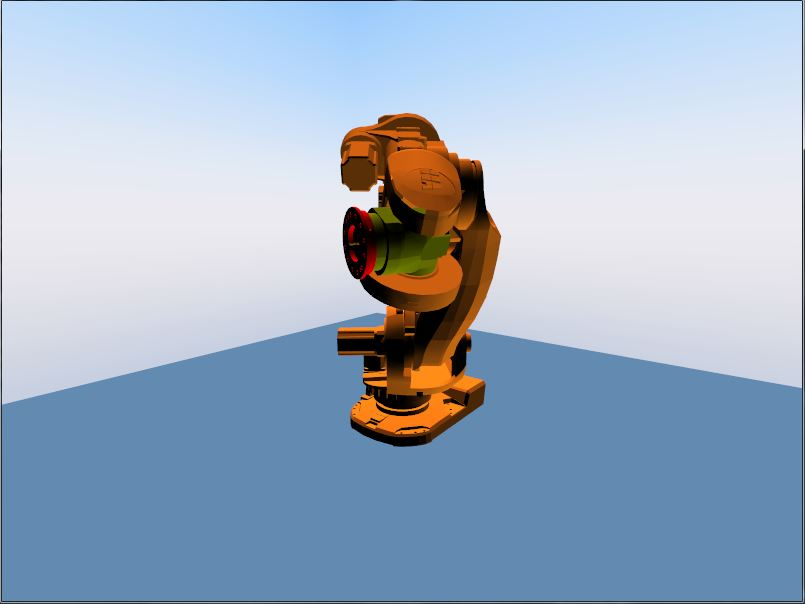
\includegraphics[width=0.25\textwidth]{figures/robot2.jpg}}
    \hfill
    \subfloat[]{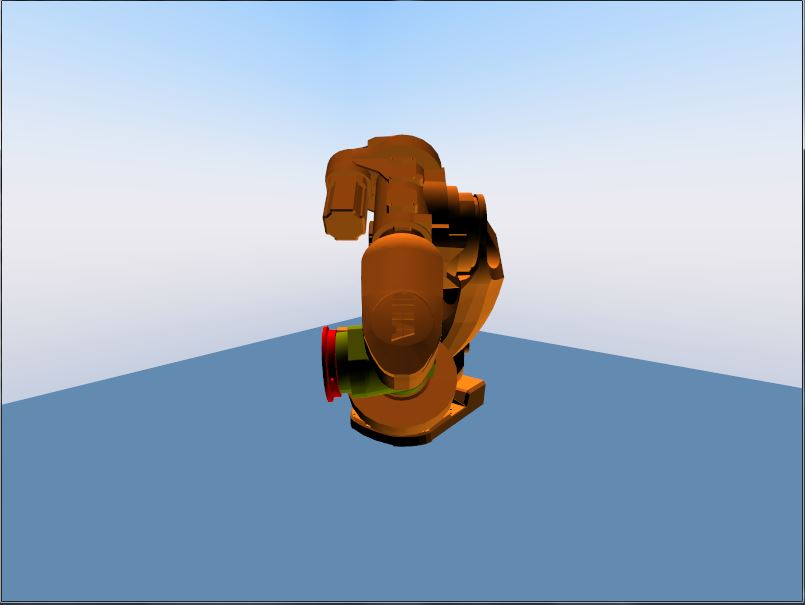
\includegraphics[width=0.45\textwidth]{figures/robot3.jpg}}
    % \hfill
    % \subfloat[]{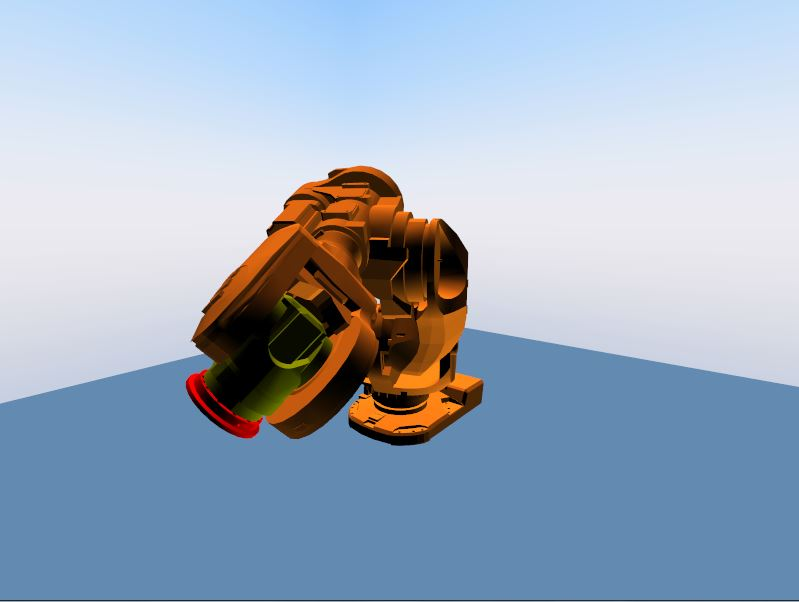
\includegraphics[width=0.25\textwidth]{figures/robot4.jpg}}
    \\
    \subfloat[]{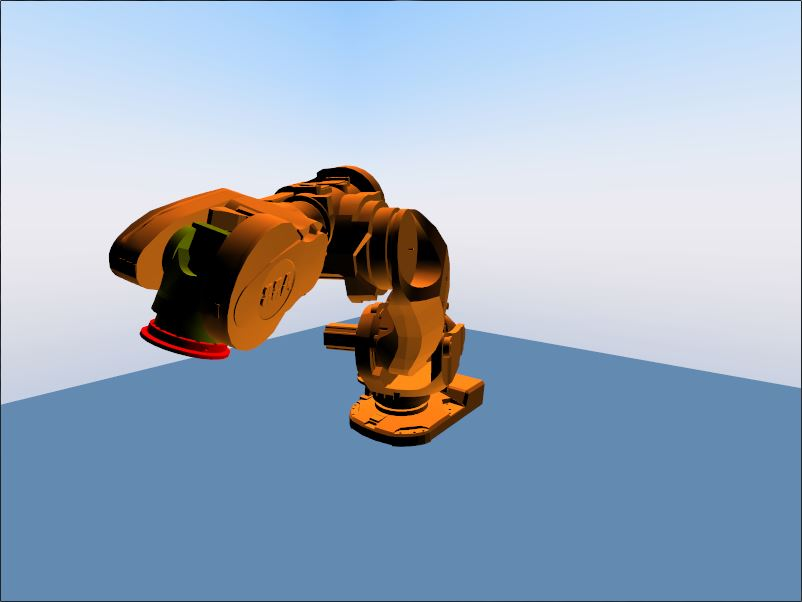
\includegraphics[width=0.45\textwidth]{figures/robot5.jpg}}
    % \hfill
    % \subfloat[]{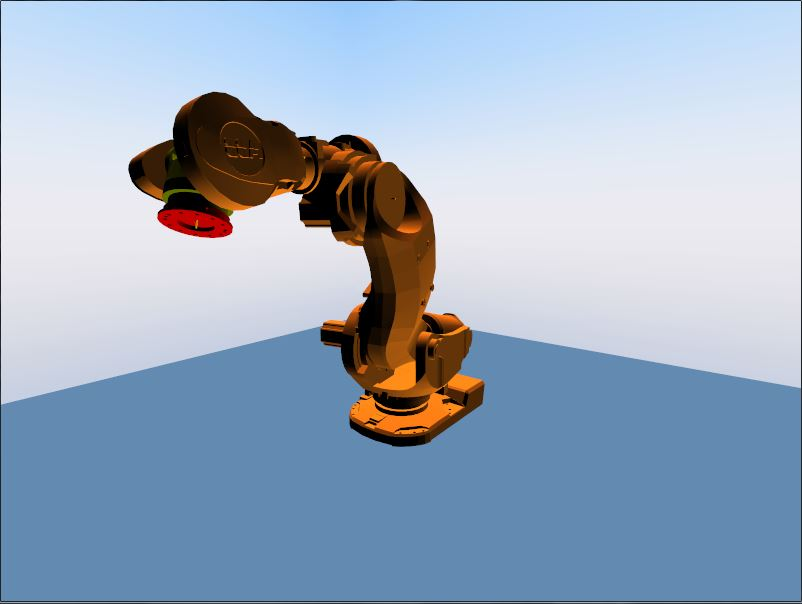
\includegraphics[width=0.25\textwidth]{figures/robot6.jpg}}
    \hfill
    \subfloat[]{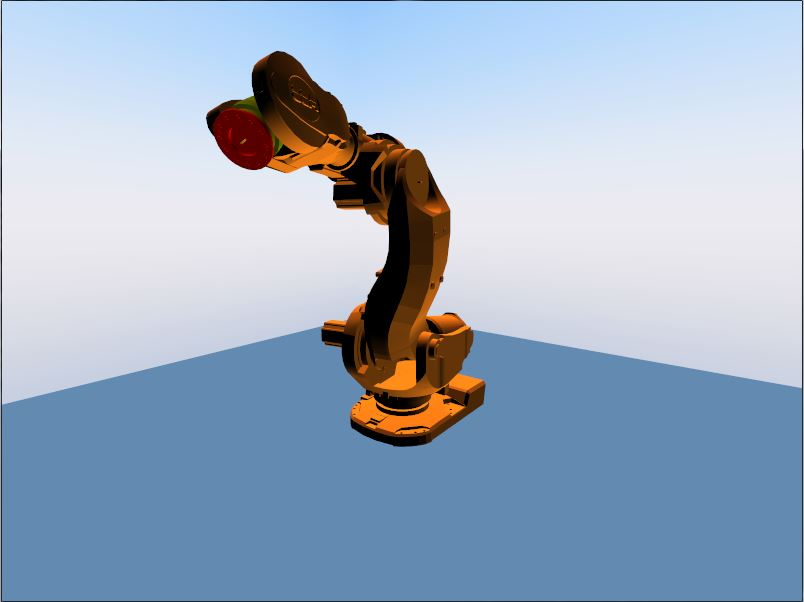
\includegraphics[width=0.45\textwidth]{figures/robot7.jpg}}
    % \hfill
    % \subfloat[]{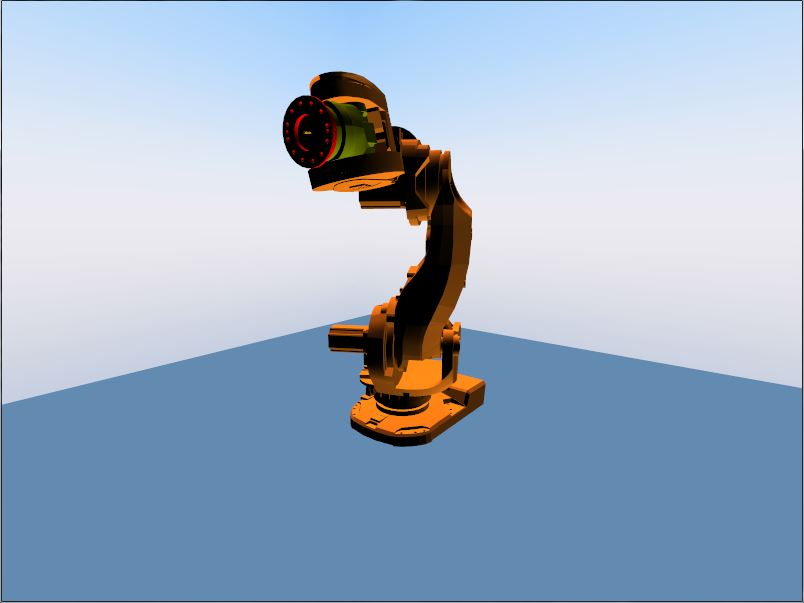
\includegraphics[width=0.25\textwidth]{figures/robot8.jpg}}
    \DIFdelbeginFL %DIFDELCMD < 

%DIFDELCMD <     %%%
\DIFdelendFL \caption{Simulation \DIFaddbeginFL \DIFaddFL{ 
\cite{tasora2015chrono}  
}\DIFaddendFL of \DIFdelbeginFL \DIFdelFL{a }\DIFdelendFL \DIFaddbeginFL \DIFaddFL{an industrial }\DIFaddendFL 6-DOF robot whose end-effector\DIFaddbeginFL \DIFaddFL{, equipped with a painting tool, }\DIFaddendFL interpolates between \DIFaddbeginFL \DIFaddFL{various }\DIFaddendFL key poses using \DIFdelbeginFL \DIFdelFL{our }\DIFdelendFL \DIFaddbeginFL \DIFaddFL{the proposed }\DIFaddendFL algorithm \DIFaddbeginFL \DIFaddFL{in association with a spatial motion}\DIFaddendFL . \DIFaddbeginFL \DIFaddFL{The provided example illustrates one of the many possible applications suitable for the algorithm.}\DIFaddendFL }
    \label{fig:chrono_robot}
\end{figure*}

%-------------------------------------------------------------------------------
\DIFaddbegin \section{\DIFadd{Benchmarks}}
\label{sec:benchmarks}
\DIFadd{In order to show that the computational effort of the proposed method is competitive with respect to other interpolation methods, we implemented a dedicated benchmark. In particular, we tested the interpolation of different number of key frames, evaluating 1E6 of intermediate samples for each. The same test has been repeated 100 times for each scenario, and the average values of computational time have been reported in Table \ref{tab:benchmark_time}. One can observe that the proposed method is indeed competitive with SLERP for a reasonably low number of given poses and, despite the progressive increase of time in function of the key frames number, its CPU time is still shorter than the 2\textsuperscript{nd}-order quaternion B-Spline and the SQUAD method. 
}

\DIFadd{The benchmarks have been computed on a Intel\textsuperscript{\textregistered} Core\textsuperscript{\texttrademark} i7-10510U CPU, clocked at  
1.80 GHz
, with 4 physical cores and  
16 GB  
of RAM. The linear algebra formulas for the benchmark have been implemented in C++ in the Chrono::Engine open-source library  
\cite{tasora2015chrono} 
, enabling the /O2 compiler optimization flag on the MSVC compiler, and using a single thread. In search of a fair comparison, no special optimization techniques have been put in place: in fact, the performance of the methods can be further improved using advanced programming techniques such as ASM assembly directives and AVX2 vectorization, that we have not considered at the moment.
}

\begin{table}[tp]
	\centering
	\caption{\DIFaddFL{Computation time required for the interpolation of different numbers of given frames by the discussed methods, expressed in $\SI{}{ms}$. The test involves the evaluation of 1E6 intermediate samples and has been repeated 100 times for each of them (average values reported).}}
	\setlength{\tabcolsep}{3pt}
	\begin{tabular}{c|ccccc}
		\toprule
		& \DIFaddFL{SLERP }& \DIFaddFL{B-Spline2 }& \DIFaddFL{SQUAD }& \DIFaddFL{Proposed method }\\
		\midrule
        \DIFaddFL{4 key frames }& \DIFaddFL{48.2 }& \DIFaddFL{479.1 }& \DIFaddFL{494.5 }& \DIFaddFL{66.1 }\\
        \DIFaddFL{50 key frames }& \DIFaddFL{49.6 }& \DIFaddFL{483.6 }& \DIFaddFL{524.1 }& \DIFaddFL{142.0 }\\
        \DIFaddFL{100 key frames }& \DIFaddFL{50.6 }& \DIFaddFL{491.9 }& \DIFaddFL{543.0 }& \DIFaddFL{194.1 }\\
		\bottomrule
	\end{tabular}
	\label{tab:benchmark_time}
\end{table}

\DIFadd{Table \ref{tab:benchmark_dist} compares a measure of the total angular distance required by each of the methods discussed to interpolate the same 100 random key frames. It is observable that, as expected, the proposed algorithm travels a longer path with respect to SLERP but, in exchange, smoothly interpolates all the given poses. On the other hand, the angular distance travelled is slightly less if compared to SQUAD. At last, the 2\textsuperscript{nd}-order quaternion B-Spline presents the shortest angular path of all methods, but sacrifices the exact passage among all the given key frames.
}

\begin{table}[tp]
	\centering
	\caption{\DIFaddFL{Example of angular distance travelled to interpolate the same 100 random key frames by the discussed methods, expressed in $\SI{}{rad}$.}}
	\setlength{\tabcolsep}{3pt}
	\begin{tabular}{c|cccc}
		\toprule
	    & \DIFaddFL{SLERP }& \DIFaddFL{B-Spline2 }& \DIFaddFL{SQUAD }& \DIFaddFL{Proposed method }\\
		\midrule
        \DIFaddFL{Angle }& \DIFaddFL{112.6 }& \DIFaddFL{84.2 }& \DIFaddFL{124.5 }& \DIFaddFL{117.1 }\\
		\bottomrule
	\end{tabular}
	\label{tab:benchmark_dist}
\end{table}



%DIF > -------------------------------------------------------------------------------
\DIFaddend \section{Conclusions}
\label{sec:conclusions}
We proposed a practical method, based on the composition of rotations and simple polynomials, that provides a smooth interpolation between an arbitrary number of given angular poses. The algorithm is rooted on repeated SLERP interpolation segments smoothly connected by suitable fillet tracts. The duration of the different segments can be arbitrarily modified by the user to optimize the trajectory. The methodology intrinsically generates transitions in orientation which preserve the continuity of angular position, velocity and acceleration. The mathematical formulation is simple \DIFaddbegin \DIFadd{because it involves simple combination of rotations }\DIFaddend and the computational burden is \DIFdelbegin \DIFdel{very limited}\DIFdelend \DIFaddbegin \DIFadd{limited, as showed by the provided benchmark}\DIFaddend . It is easy to generate constant angular velocity trajectories as well as motions with predefined velocity profiles. \DIFaddbegin \DIFadd{Specific angular velocity vectors can be imposed in the control points. }\DIFaddend The comparison with other known methodologies shows that:
1) with respect to SLERP, it does not \DIFdelbegin \DIFdel{have velocity discontinuities }\DIFdelend \DIFaddbegin \DIFadd{present velocity discontinuities but slightly increases angular distance covered and computation time}\DIFaddend ;
2) with respect to a \DIFaddbegin \DIFadd{quaternion }\DIFaddend B-Spline, the computational burden is lower \DIFdelbegin \DIFdel{, }\DIFdelend and it is easier to impose the exact crossing of \DIFaddbegin \DIFadd{the }\DIFaddend assigned angular positions;
3) with respect to SQUAD, the angular distance covered is smaller\DIFaddbegin \DIFadd{, the computation time is lower }\DIFaddend and there are no oscillations in velocities. 
\DIFdelbegin \DIFdel{Finally, the }\DIFdelend \DIFaddbegin 

\DIFadd{The }\DIFaddend proposed methodology can be easily used to generate 3D \DIFdelbegin \DIFdel{mechanical motions or to solve computer graphicsproblems; }\DIFdelend \DIFaddbegin \DIFadd{motions of mechanical parts and it can be useful in those cases where a simple formula for smooth interpolation of key poses is desired: we can mention, for instance, biomechanics (when one must interpolate between sample poses obtained via motion capture experiments) as well as computer graphics, video games and robotics. Finally, }\DIFaddend a possible application related to industrial robots has been presented to this end. 


%-------------------------------------------------------------------------------

\clearpage
\appendix

%-------------------------------------------------------------------------------
\section{Rotation matrices}
\label{app:RotatMatrix}
The present appendix section recalls, without proof, some fundamental notions on rotation matrices \cite{joe-angoli,joe-prj} and defines the notation used throughout this paper.

\subsection{Conversion between different reference frames}
\label{app:RotatMatrix1}
The conversion of vectors between two different reference frames $(i)$ and $(j)$ can be obtained by means of the rotation matrix $R_{ji}$ representing their relative pose. Naming $\vect{v}_{(i)}$ the original three-components vector and $\underline{\vect{v}}_{(i)}$ its skew-symmetric matrix representation as in
\begin{equation}
    \vect{v}_{(i)} = \left[
    \begin{array}{c}
            v_{xi} \\
            v_{yi} \\
            v_{zi} \\
    \end{array}
    \right] \qquad {\underline{\vect{v}}_{(i)}} = \left[
    \begin{array}{ccc}
            0 & -v_{zi} & v_{yi} \\
            v_{zi} & 0 & -v_{xi} \\
            -v_{yi} & v_{xi} & 0 \\
    \end{array}
    \right]
    \label{eq:VV_}
\end{equation}
we obtain the following notable relations:
\begin{equation}
    \vect{v}_{(j)} = R_{ji} \vect{v}_{(i)} \qquad\qquad \underline{\vect{v}}_{(j)} = R_{ji} \underline{\vect{v}}_{(i)} R_{ij}
    \label{eq:cambioRif}
\end{equation}
Each column of matrix $R_{ji}$ contains the unit vectors of the axes of frame  $(i)$ as seen by frame $(j)$
\begin{equation}
    R_{ji} = \left[
    \begin{array}{c|c|c}
        x_{x} & y_{x} & z_{x} \\
        x_{y} & y_{y} & z_{y} \\
        x_{z} & y_{z} & z_{z} \\
    \end{array}
    \right]
     = \left[
    \begin{array}{c|c|c}
         &  &  \\
        \vect{u}_x & \vect{u}_y & \vect{u}_z \\
         &  & \\
    \end{array}
    \right]
    \label{eq:column}
\end{equation}
This matrix also represent the orientation (or attitude) of frame $(i)$ with respect to frame $(j)$.

Since the presented properties hold for any frames, Eq. \ref{eq:cambioRif} can also be written as $\vect{v}_{(i)} = R_{ij} \vect{v}_{(j)}$; thus, we deduce  that
\begin{equation}
    R_{ij}=R_{ji}^{-1}
    \label{eq:inverseR}
\end{equation}
Considering that the columns of matrix $R$ in Eq. \ref{eq:column} are orthogonal to each other, we conclude that matrix $R$ itself is orthogonal and so the following properties holds
\begin{equation}
    R^{-1}=R^T \qquad\qquad \det(R)=\pm 1
    \label{eq:RiRT}
\end{equation}
The determinant is positive if both frames are right or left, and negative if one is right and the other is left.

In case of multiple frame change it is possible to use the following composition rule
\begin{equation}
    R_{ik} = R_{ij} R_{jk}
    \label{eq:MultiR}
\end{equation}


\subsection{Rotation of vectors and frames}
\label{app:RotatMatrix2}
Let us consider a vector $\vect{v} = [v_x\ v_y\ v_z]^T$ to be rotated from a starting position $\vect{v}_s$ to reach a final position $\vect{v}_f$ of an angle $\varphi$ around axis $\vect{u}$. This transformation can be represented by matrix $R$ with:
\begin{equation}
    \vect{v}_f = R \vect{v}_s 
    \qquad\qquad 
    R(\vect{u},\varphi) = 1 + \underline{\vect{u}}\sin\varphi + \underline{\vect{u}}^2(1-\cos\varphi)
    \label{eq:rotat_phi_u}
\end{equation}
Of course the vectors and the unit vector $\vect{u}$ must be represented by their projections in the same reference frame that we can indicate (for instance) as $(r)$. If a rotation is expressed in frame $(r)$, the same rotation in a different frame $(s)$ will be (see Eq. \ref{eq:cambioRif})
\begin{equation}
    R_{(s)}= R_{sr} R_{(r)} R_{rs}
    \label{eq:changeRif}
\end{equation}
Let's indicate by subscript $(0)$ the absolute reference system in which we describe the angular position of two frames (1) and (2).
Remembering Eq. \ref{eq:column}, if we rotate the frame whose attitude is $R_{01}$ of an angle $\varphi$ around an axis $\vect{u}$ to reach the orientation $R_{02}$, we can write (each column of $R$ is transformed according to Eq. \ref{eq:cambioRif}):
\begin{equation}
    R_{02}=\overline{R}(\vect{u}_{(0)},\varphi) R_{01}
    \label{eq:rotR01_02}
\end{equation}
So, if the initial angular position $R_{01}$ and the final one $R_{02}$ are known, the rotation which transform the former to the latter is determined in frame $(0)$ as
\begin{equation}
    \overline{R}(\vect{u}_{(0)},\varphi) = R_{02} R_{01}^{-1} = R_{02} R_{10}
    \label{eq:RotFrame0}
\end{equation}
Remembering Eqs. \ref{eq:cambioRif}, \ref{eq:MultiR} and \ref{eq:changeRif}, if the result is sought in frame $(1)$ or $(2)$, the rotation becomes simply
\begin{equation}
   \overline{R}(\vect{u}_{(1)}, \varphi) = \overline{R}(\vect{u}_{(2)},\varphi) = R_{12}
    \label{eq:RRR12}
\end{equation}
Once the matrix $\overline{R}$ is known, the rotation angle and axis may be extracted as
\begin{equation}
    \begin{array}{l}
        c=\cos\varphi=\frac{x_{x}+y_{y}+z_{z}-1}{2}\\[2ex] s=\sin\varphi=\frac{\sqrt{(y_{z}-z_{y})^2+(x_{z}-z_{x})^2+(x_{y}-y_{x})^2}}{2}\\[2ex]
        \varphi=\operatorname{atan2}(s,c); \hspace{4ex} \pi < \varphi \leq \pi\\
        \ \\
        \underline{\vect{u}}=\cfrac{1}{2\sin\varphi} \left(\overline{R}-\overline{R}^T\right)
        \qquad
        \begin{array}{l}
          u_x=\frac{(y_{z}-z_{y})}{2\sin \varphi} \\[2ex]
          u_y=\frac{(z_{x}-x_{z})}{2\sin \varphi} \\[2ex]
          u_z=\frac{(x_{y}-y_{x})}{2\sin \varphi}
        \end{array}
        \qquad\qquad
        \sin\varphi\ne 0
    \end{array}
    \label{eq:extract}
\end{equation}

%-------------------------------------------------------------------------------
\section{Quaternions, rotations and exponentials}
\label{app:Quaternion}

\DIFaddbegin \DIFadd{We list some properties of quaternions that are used in interpolation schemes discussed in this work. 
}

\DIFaddend \subsection{Main properties}
\DIFdelbegin \DIFdel{A second and efficient way to represent rotations }\DIFdelend \DIFaddbegin \DIFadd{Rotations }\DIFaddend in 3D space \DIFdelbegin \DIFdel{is by means of Euler parameters(not to be confused with Euler angles). These are four scalars $\quat{q} = \{ q_0,q_1,q_2,q_3 \}$ obtained by the }\DIFdelend \DIFaddbegin \DIFadd{can be represented by four scalars $q_0,q_1,q_2,q_3$
%DIF > $\quat{q} = \{ q_0,q_1,q_2,q_3 \}$, 
called Euler parameters, related to the rotation }\DIFaddend angle $\varphi$ and \DIFdelbegin \DIFdel{the }\DIFdelend \DIFaddbegin \DIFadd{rotation }\DIFaddend axis $\vect{u}$ \DIFdelbegin \DIFdel{describing the rotation }\DIFdelend as \cite{tasora}
%
\begin{equation}
    \begin{array}{c}
    	{q}_0 = \cos \left(\frac{\varphi}{2} \right) \\[2ex]
     	{q}_1 = u_x \sin \left(\frac{\varphi}{2}\right)  \quad
     	{q}_2 = u_y \sin \left(\frac{\varphi}{2}\right)  \quad
     	{q}_3 = u_z \sin \left(\frac{\varphi}{2}\right) 	
    \end{array}
    \label{eq:defQ}
\end{equation}
By the definitions (Eq. \ref{eq:defQ}), the following constrain holds: $q_0^2+q_1^2+q_2^2+q_3^2=1$.
Euler parameters can be interpreted as unit-length \textit{quaternions} $\quat{q} \in \mathbb{H}_1$, $||\quat{q}||=1$, that is a subset of quaternion hyper-complex numbers $\mathbb{H}$ written as
\begin{equation}
    \quat{q}= q_0 + q_1\: i + q_2\: j + q_3\: k  
    \label{eq:quaternion}
\end{equation}
In this representation \cite{hamilton1844ii}, the following properties hold
\begin{equation}
    \begin{array}{c}
        i^2=j^2=k^2=-1\\[2ex]
        ij=-ji=k;\qquad jk=-kj=i; \qquad ki=-ik=j
    \end{array}
    \label{eq:quaternionProp}
\end{equation}

Quaternions can be written succinctly with the notation $\quat{q}=[q_{s},\vect{q}_{v}]$, showing the \textit{scalar part} $q_s=q_0$ and the \textit{vector part} $\vect{q}_v = \{q_1, q_2, q_3\}$; this simplifies the expression of quaternion multiplication. In fact, with $\quat{\tau}\in\mathbb{H}$, \DIFdelbegin \DIFdel{$\quat{\rho}\in\mathbb{H}$}\DIFdelend \DIFaddbegin \DIFadd{$\quat{\eta}\in\mathbb{H}$}\DIFaddend , by means of the properties \eqref{eq:quaternionProp} one obtains the product formula:
\begin{align} 
\quat{\tau} \: \DIFdelbegin %DIFDELCMD < \quat{\rho} %%%
\DIFdelend \DIFaddbegin \quat{\eta} \DIFaddend = [ \tau_{s}\DIFdelbegin \DIFdel{\rho_{s} }\DIFdelend \DIFaddbegin \DIFadd{\eta{s} }\DIFaddend - \vect{\tau}_{v}\cdot\DIFdelbegin %DIFDELCMD < \vect{\rho}%%%
\DIFdelend \DIFaddbegin \vect{\eta}\DIFaddend _{v}, \;
\tau_{s}\DIFdelbegin %DIFDELCMD < \vect{\rho}%%%
\DIFdelend \DIFaddbegin \vect{\eta}\DIFaddend _{v} + \rho_{s}\DIFdelbegin %DIFDELCMD < \vect{\tau}%%%
\DIFdelend \DIFaddbegin \vect{\eta}\DIFaddend _{v} + \DIFdelbegin %DIFDELCMD < \vect{\tau}%%%
\DIFdelend \DIFaddbegin \vect{\eta}\DIFaddend _{v} \times \DIFdelbegin %DIFDELCMD < \vect{\rho}%%%
\DIFdelend \DIFaddbegin \vect{\eta}\DIFaddend _{v} ]
	%\label{eq:quatproduct}
\end{align}

A rotation matrix can be constructed from a quaternion as
\begin{equation}
\begin{array}{rl}
R(\quat{q})& =\left[
	\begin{matrix}
	 q_0^2 + q_1^2 - q_2^2 - q_3^2  &  2(q_1 q_2 - q_3 q_0)   &  2(q_1 q_3 + q_2 q_0)  \cr
	 2(q_1 q_2 + q_3 q_0)  &  q_0^2 - q_1^2 + q_2^2 - q_3^2  &   2(-q_1 q_0 + q_2 q_3) \cr
     2(q_1 q_3 - q_2 q_0)  &  2(q_1 q_0 + q_2 q_3)  & q_0 ^2 -q_1^2 -q_2^2 + q_3^2   
	\end{matrix}
	\right] =\\
&=\left[
\begin{array}{ccc}
        x_{x}            &       y_{x}           &       z_{x}  \\
        x_{y}            &       y_{y}           &       z_{y}  \\
        x_{z}            &       y_{z}           &       z_{z}
\end{array}\right]
\end{array}
\label{new_eq:fromQtoR}
\end{equation}
Vice versa, if the matrix $R$ is known, the elements of the quaternion are extracted as
\begin{equation}
\begin{array}{l}
q_0=\frac{1}{2} \sqrt{t+1},\qquad t=x_{x}+y_{y}+z_{z};\\[2ex]
  q_1=\frac{(y_{z}-z_{y})}{4\: q_0};\qquad \qquad
  q_2=\frac{(z_{x}-x_{z})}{4\: q_0};\qquad \qquad
  q_3=\frac{(z_{y}-y_{x})}{4\: q_0}
\label{eq:fromRtoQ}
\end{array}
\end{equation}
which are valid for $q_0 \neq 0$; while for $q_0=0$ the following relations hold
\begin{equation}
\begin{array}{l}
        \left\{
        \begin{array}{c}
                4 q_2 q_3 =y_{z}+z_{y} \\
                4 q_1 q_3 =z_{x}+x_{z} \\
                4 q_1 q_2 =y_{x}+x_{y}
        \end{array}
        \right.
\ \\
{\small
                q_1=\pm \sqrt{\cfrac{x_{x}+1}{2}} \qquad
                q_2=\pm \sqrt{\cfrac{y_{y}+1}{2}} \qquad
                q_3=\pm \sqrt{\cfrac{z_{z}+1}{2}}
}
\end{array}
\label{eq:fromRtoQ2}
\end{equation}

A sequence of rotations can be represented by the product of two quaternions:
similarly to $R_t=R(\quat{q}_{2}) R(\quat{q}_{1})$, the quaternion $\quat{q}_{t}$, expressing the final rotation obtained by the sequence of a rotation $\quat{q}_{1}$ followed by a rotation $\quat{q}_{2}$, is obtained as 
\begin{equation}
    \quat{q}_{t}=\quat{q}_{2}\: \quat{q}_{1}
\end{equation}

We denote the quaternion conjugate of \DIFdelbegin \DIFdel{$\quat{\rho}$ as $\quat{\rho}^*$}\DIFdelend \DIFaddbegin \DIFadd{$\quat{q}$ as $\quat{q}^*$}\DIFaddend , with $\quat{q}^*= q_0 - q_1 i  - q_2 j -  q_3 k$. This corresponds to an inverse rotation and in fact one has:
\begin{equation}
    \amatr{R}(\quat{q}^*) = \amatr{R}(\quat{q})^T = \amatr{R}(\quat{q})^{-1} 
\end{equation}

Quaternions, as well as rotation matrices define an algebraic structure over a differential manifold with properties of closure, associativity, presence of identity element and inverse element, hence they belong to a \textit{Lie group}. The Lie group of rotation matrices is called $\mathsf{SO}(3)$, the special orthogonal group of orthogonal matrices with $\text{det}=1$. The Lie group of unimodular quaternions $\mathbb{H}_1$ is topologically isomorphic to the $\mathsf{S}^3$ sphere, as such it is a double cover of $\mathsf{SO}(3)$, hence two distinct opposite quaternions represent the same rotation matrix $\amatr{R} \in \mathsf{SO}(3)$.

Given a $\gamma(t) : \mathbb{R} \rightarrow \mathsf{SO}(3)$ be a one parameter sub-group of $\mathsf{SO}(3)$ for which $\gamma(0) = I$, an \emph{exponential map} is defined as $\exp(\amatr{\Theta})=\gamma(1)$, where $\amatr{\Theta} \in \mathfrak{so}(3)$ is an element of the underlying Lie algebra. 

Rotation matrices can be built as exponential maps from elements $\amatr{\Theta} \in \mathfrak{so}(3)$ and vice versa:  
%
\begin{align}
\amatr{R}      &= \mathrm{exp}(\amatr{\Theta})=R(\DIFdelbegin \DIFdel{u}\DIFdelend \DIFaddbegin \vect{u}\DIFaddend ,\varphi) \label{Rexp}\\
\amatr{\Theta} &= \mathrm{log}(\amatr{R})=\underline{\vect{u}}\varphi \label{Rlog}
\end{align}
%
The \DIFdelbegin \DIFdel{3x3 skew-symmetric matrix $\amatr{\Theta} \in \mathfrak{so}(3)$ is also related to the rotation vector }\DIFdelend \DIFaddbegin \emph{\DIFadd{rotation vector}} \DIFaddend $\vect{\theta} \in \mathbb{R}^3$\DIFdelbegin \DIFdel{via 
%DIF < 
}\begin{align*}
    \DIFdel{\vect{\theta} }&\DIFdel{= \text{axis}(\amatr{\Theta})=\vect{u}\vartheta }\\ 
    \DIFdel{\amatr{\Theta} }&\DIFdel{=  \mathrm{skew}(\vect{\theta}) = \underline{\vect{\theta}}=\underline{\vect{u}}\vartheta
}\end{align*}%DIFAUXCMD
%DIFDELCMD < 

%DIFDELCMD < %%%
\DIFdel{For }\DIFdelend \DIFaddbegin \DIFadd{, defined for }\DIFaddend a finite rotation of angle $\varphi$ about a unit vector $\vect{u}$, \DIFdelbegin \DIFdel{it is $\vect{\theta}=\varphi \vect{u}$.
}\DIFdelend \DIFaddbegin \DIFadd{is related to the 3x3 skew-symmetric matrix $\amatr{\Theta} \in \mathfrak{so}(3)$ via 
%DIF > 
}\begin{align}
    \DIFadd{\vect{\theta} }&\DIFadd{= \text{axis}(\amatr{\Theta})=\vect{u}\varphi }\\ 
    \DIFadd{\amatr{\Theta} }&\DIFadd{=  \mathrm{skew}(\vect{\theta}) = \underline{\vect{\theta}}=\underline{\vect{u}}\varphi
}\end{align}

\DIFaddend Similarly, the exponential map of unit quaternions links $\mathbb{H}_1$ to its Lie algebra $\mathsf{Im}(\mathbb{H})$ of \emph{pure quaternions} $\vect{\rho} =  [0, \vect{\nu}]$:
%
\begin{align}
\quat{q}      &= \mathrm{exp}(\vect{\rho}) \label{eq:rexp}\\
\vect{\rho} &= \mathrm{log}(\vect{q})   \label{eq:rlog}
\end{align}
%
The exponential map \eqref{eq:rexp} can be explicitly computed using the closed-form expression 
$\exp([s,\vect{v}]) =  e^s \left[\cos(||\vect{v}||),\frac{\vect{v}}{||\vect{v}||}\sin(||\vect{v}||)\right]$, hence:
%
\begin{align}
\label{eq:at:quatexpa}
  \exp([0, \vect{\nu}]) &=  \left[\cos(||\vect{\nu}||),\frac{\vect{\nu}}{||\vect{\nu}||}\sin(||\vect{\nu}||)\right]   \\
\label{eq:at:quatexpb}
  \exp([0,\vect{u}\DIFdelbegin \DIFdel{\beta}\DIFdelend \DIFaddbegin \DIFadd{\xi}\DIFaddend ]) &=  [\cos(\DIFdelbegin \DIFdel{\beta}\DIFdelend \DIFaddbegin \DIFadd{\xi}\DIFaddend ),\vect{u}\sin(\DIFdelbegin \DIFdel{\beta}\DIFdelend \DIFaddbegin \DIFadd{\xi}\DIFaddend )]  \quad  \text{for} \; ||\vect{u}||=1
\end{align}
%
We can use the  \textrm{pure}() and \textrm{imag}() operators to convert pure quaternions  $[0,\vect{\nu}]$ from and to rotation vectors $\vect{\theta}$ by observing that \DIFaddbegin \DIFadd{$\xi =  \frac{1}{2} \varphi$, }\DIFaddend $\vect{\nu} = \frac{1}{2} \vect{\theta}$: 
\begin{align}
    \vect{\theta}  &= 2 \: \text{imag}(\vect{\rho})  \\
    \vect{\rho}    &= \tfrac{1}{2} \text{pure}(\vect{\theta})  
    \end{align}

To pass directly from rotation vector $\vect{\theta}$ to quaternion $\vect{q}=[s,\vect{v}]$, and vice versa, one can use the compact expressions:
\begin{align}
\vect{q} &= 
%\mathrm{exp}(\vect{\rho}) =
\mathrm{exp} \left( \tfrac{1}{2} \text{pure}(\vect{\theta}) \right) = 
\left[ 
\cos\left(\frac{||\vect{\theta}||}{2}\right), 
\frac{\vect{\theta} }{ ||\vect{\theta}|| } \sin\left( \frac{||\vect{\theta}||}{2}\right) 
\right] 
\label{eq:qexponential}  \\
\vect{\theta} &= 
%\mathrm{axis}(\vect{\rho}) =
2 \: \mathrm{imag} ( \text{log}(\vect{q}) ) = 
2\frac{\vect{v}}{||\vect{v}||}\tan^{-1}\left(\frac{||\vect{v}||}{s}\right) 
\label{eq:qlogarithm}
\end{align} 
Note that the last expression is singular for zero rotations, so when $||\vect{v}|| < \epsilon$ one can compute it as the simplified expression \DIFdelbegin \DIFdel{$\delta\vect{\theta} = 2 \vect{v}$}\DIFdelend \DIFaddbegin \DIFadd{$\vect{\theta} = 2 \vect{v}$}\DIFaddend . Also note that rather than using $\tan^{-1}()$ it is advisable to use $\mathrm{atan2}()$.

As a special case, the scalar exponential of a quaternion boils down to:
\begin{align}
    \nonumber
        \quat{q}^{\:t} &= \left[ \cos(\DIFdelbegin \DIFdel{\beta}\DIFdelend \DIFaddbegin \DIFadd{\xi}\DIFaddend ),\vect{u}\sin(\DIFdelbegin \DIFdel{\beta}\DIFdelend \DIFaddbegin \DIFadd{\xi}\DIFaddend ) \right]^t \\ 
    \label{eq:at:quatpowd}
      \quat{q}^{\:t}  &= \left[ \cos(\DIFdelbegin \DIFdel{\beta }\DIFdelend \DIFaddbegin \DIFadd{\xi }\DIFaddend t),\vect{u}\sin(\DIFdelbegin \DIFdel{\beta }\DIFdelend \DIFaddbegin \DIFadd{\xi }\DIFaddend t) \right]
\end{align}
\DIFaddbegin 

\DIFadd{Finally, one can see that the interpolation method of Eq.\ref{eq:raccordo} can be expressed also via a double product of quaternions:
}\begin{align}
        \DIFadd{\quat{q} = \quat{q}_{01}
        \mathrm{exp} \left( \tfrac{1}{2} \text{pure}(\vect{u}_1 \alpha) \right)
        \mathrm{exp} \left( \tfrac{1}{2} \text{pure}(\vect{u}_2 \beta) \right)
         \label{eq:at:raccordo_quaternioni}
}\end{align}
\DIFadd{or equivalently as 
%DIF > $\quat{q} = \quat{q}_{01}  \quat{q}_{12}^{\alpha/\overline{\alpha}} \quat{q}_{23}^{\beta/\overline{\beta}}$
$\quat{q} = \quat{q}_{01}
\mathrm{exp} \left( \alpha \, \mathrm{log}(\quat{q}_{01}^* \quat{q}_{02})  \right)
\mathrm{exp} \left( \beta \, \mathrm{log}(\quat{q}_{02}^* \quat{q}_{03})  \right)
$
.
}\DIFaddend 

\subsection{Velocity and acceleration} 
%From the definition of the exponential map, it holds 
%$\gamma(t)=\exp(t \amatr{\Omega})$, with $\gamma(0)=I$,
%therefore
%$\dot{\gamma}(0)=\amatr{\Omega}$.
%For a more generic case with $R(t)=\gamma(t) R_0$, $R(0)=R_0$, one multiplies both terms of the %first equation by $R_0$ to obtain 
%$\gamma(t) R_0 = \exp(t\amatr{\Omega}) R_0$, \hl{***per omega costante?***}
%then differentiates to obtain
%$\dot{R}(t) = \amatr{\Omega} R_0$, where $\amatr{\vect{\omega}} = \underline{\vect{\omega}}_e$ is the skew-symmetric matrix that contains the angular velocity $\vect{\omega}_e$ expressed in absolute (extrinsic) coordinates. This is written succinctly as:
Introducing the vector of angular velocity $\vect{\omega}_e$ expressed in absolute (extrinsic) coordinates, one has
\begin{align}
\dot{R} = \underline{\vect{\omega}}_e R\qquad
\label{eq:Adot}
\end{align}
Similarly, by a second differentiation, and introducing the (extrinsic) angular acceleration $\vect{\dot{\omega}}_e$, one has
\begin{align}
\ddot{R}=\underline{\vect{\dot{\omega}}}_e R+\underline{\vect\omega}^2_e R\qquad
\label{eq:Adotdot}
\end{align}

Given quaternion derivatives, it is possible to compute extrinsic angular velocity and extrinsic angular acceleration, or vice versa, using the following relations:
\begin{align}
\vect{\omega}_e &= 2 \; {F}(q\conj) \dot{\quat{q}} \\
\vect{\dot{\omega}}_e &= 2 \; {F}(q\conj) \ddot{\quat{q}} \\
\dot{\quat{q}} &= \tfrac{1}{2} {F}(q\conj)^T  \vect{\omega}_e  \\
\ddot{\quat{q}} &= \tfrac{1}{2} {F}(\dot{q}\conj)^T  \vect{\omega}_e + \tfrac{1}{2} {F}(q\conj)^T  \vect{\dot{\omega}}_e 
\end{align}
with the introduction of the matrix 
\begin{align}
\label{eq:at:rotFm} 
	\amatr{F(q)}&= 
	\left[
	\begin{matrix}
	 +q_1 & +q_0  & +q_3  & -q_2  \cr
	 +q_2 & -q_3  & +q_0  & +q_1  \cr
	 +q_3 & +q_2  & -q_1  & +q_0  
	\end{matrix}
	\right]
\end{align}

%-------------------------------------------------------------------------------
\section{Other interpolation schemes}
\label{app:otherinterpolations}
In the following, for completeness, we briefly describe other interpolation methods that are popular in literature and which we used in our benchmarks for comparisons.

\subsection{SLERP}
The spherical linear interpolation (SLERP \cite{shoemake1985animating}), with domain $t \in [0,1]$, interpolates two quaternions
$\quat{q}_a$ and $\quat{q}_b$ using the exponential formula \eqref{eq:at:quatpowd} to compute:
%
\begin{align}
\label{eq:at:quatrotSLERPa}
 \quat{q}(t) &= f_{\text{SLERP}}(\quat{q}_a,\quat{q}_b,t)  \nonumber \\
 &= \left( \quat{q}_b \quat{q}_a^{*} \right)^t \quat{q}_a
\end{align}

The norm of the quaternion is guaranteed to be unit length. The rotation matrix $R(t)$, if needed, can be computed from $\quat{q}(t)$ using \eqref{new_eq:fromQtoR}.


\subsection{SQUAD}
This method, also presented by Shoemake \cite{Shoemake1987QuaternionCA}, performs a cubic interpolation with domain $t \in [0,1]$ passing exactly at two extreme attitudes expressed by rotation quaternions $\quat{q}_1$ and $\quat{q}_2$, and approaching two intermediate control quaternions $\quat{p}_1$ and $\quat{p}_2$ similarly to cubic Bezier curves. It does this by using nested calls to the SLERP function, that is:
\begin{align}
\label{eq:at:quatrotSQUAD}
 \quat{q}(t) &=  f_{\text{SQUAD}}(\quat{q}_1,\quat{p}_1,\quat{p}_2,\quat{q}_2,t) \nonumber \\
  &= f_{\text{SLERP}}( f_{\text{SLERP}}(\quat{q}_1,\quat{q}_2 ,t),  f_{\text{SLERP}}(\quat{p}_1,\quat{p}_2 ,t), 2 t (1-t) )
\end{align}
In our implementation, an arbitrary sequence of $\quat{q}_i$ quaternions can be provided, to be interpolated exactly: for each span, the two intermediate $\quat{p}_1$ and $\quat{p}_2$ quaternions are computed to ensure $C^2$ continuity across span using the following formula: assuming the $i$-th span with quaternions 
$\{ \quat{q}_i, \quat{p}_i, \quat{p}_{i+1}, \quat{q}_{i+1}\}$, we compute 
\begin{align}
\label{eq:at:quatrotSQUADinner}
 \quat{p}_i &= \quat{q}_i \mathrm{exp} \left( - \frac{1}{4} \left( \mathrm{log}(\quat{q}_i^* \quat{q}_{i+1}) + \mathrm{log}(\quat{q}_i^* \quat{q}_{i-1})  \right)  \right)  
\end{align}

\subsection{Quaternion B-splines}
For completeness in the following we report the formulation of quaternion B-splines, that was put forward by Kim et al. in the nineties \cite{kim1995ac}, and that is used in our benchmarks for comparison with our method. 
We assumes a sequence of $n$ given quaternion control points $\quat{q}_i$, and a knot vector with $t_i$ knots. We assume that conventional B-spline basis functions $B_{i,k}(t)$ can be computed as $(k-1)$-order piecewise polynomials with non-zero support in $[t_i,t_{i+k}]$. Defining the cumulative form of the basis:
\begin{equation}
    \tilde{B}_{i,k}(t) = \sum_{j=1}^{n} B_{j,k}(t)  
\end{equation}
one can compute the interpolated quaternion with the expression
\begin{equation}
    \quat{q}(t) = \quat{q}_0^{\tilde{B}_{0,k}(t)} \prod_{i=1}^{n} \exp \left( \log(\quat{q}_{i-1}^* \quat{q}_i) \tilde{B}_{i,k}(t) \right)
\end{equation}
This method produces an interpolation that is $C^{k-2}$ continuous. For $k=2$ it boils down to the simple SLERP interpolation, but for higher orders, differently from the other interpolation schemes presented in this paper, it does not pass through the $\quat{q}_i$ values (except if knot multiplicity is enforced, for instance at the beginning and at the end of the curve).

\subsection{Triplets of angle functions}
Assuming that one computes a rotation matrix as a sequence of three rotations about three axis, one has
\begin{equation}
    R = R(\alpha,\beta,\gamma) = R(\gamma) R(\beta) R(\alpha)
\end{equation}
where $R(\alpha)$, $R(\beta)$ and $R(\gamma)$ are matrices of rotation about the X, Y, or Z orthogonal axes, in whatever user predefined order. 
If one provides three scalar functions for the three angles $\alpha(t)$, $\beta(t)$, $\gamma(t)$, one can obtain 
\begin{equation}
    R(t) = R(\gamma(t)) R(\beta(t)) R(\alpha(t))
\end{equation}
Similarly, if using quaternions, one would compute the double product
$\quat{q}(t)=\quat{q}(\gamma(t))\quat{q}(\beta(t))\quat{q}(\alpha(t))$. For instance, $\alpha(t)$ could be a B-spline or Bezier interpolation between $\alpha_i$ corresponding to $n$ keyframe rotations, and similarly for $\beta(t)$, $\gamma(t)$.
In any case, whatever the choice of ordering of the sequence of the three axis, there is always a singular attitude for whom, passing close to it, curves may degenerate in sharp and unpredictable oscillations. For this reason, interpolations based on triplets of angle functions are seldom used. 

%-------------------------------------------------------------------------------
\section{Polynomial motion law}
\label{app:poly5}
In this section we summarize the quantities needed to define a five-degree polynomial motion law with assigned initial and final conditions of position, velocity and acceleration. If we name
\begin{itemize}
    \item[$s_i$, $s_f$]: initial and final position
    \item[$v_i$, $v_f$]: initial and final velocity
    \item[$a_i$, $a_f$]: initial and final acceleration
    \item[$\Delta s$]$= s_f - s_i$
\end{itemize}
and we impose the following relations
\begin{equation}
    \begin{array}{l}
        A = s_i\\
        B = v_i\\
        C = \cfrac{a_i}{2}\\
        D = \cfrac{a_f - 3a_i}{2T} - \cfrac{6v_i + 4v_f}{T^2} + \cfrac{10 \Delta s}{T^3}\\
        E = \cfrac{3a_i - 2a_f}{2T^2} + \cfrac{8v_i + 7v_f}{T^3} - \cfrac{15 \Delta s}{T^4}\\
        F = \cfrac{a_f - a_i}{2T^3} - \cfrac{3(v_i + v_f)}{T^4} + \cfrac{6 \Delta s}{T^5}\\
    \end{array}
\end{equation}
we may formulate the desired motion law and its derivatives as follows:
\begin{equation}
    \begin{array}{l}
        s(t) = Ft^5 + Et^4 + Dt^3 + Ct^2 + Bt + A\\
        \dot{s}(t) = 5Ft^4 + 4Et^3 + 3Dt^2 + 2Ct + B\\
        \ddot{s}(t) = 20Ft^3 + 12Et^2 + 6Dt + 2C\\
    \end{array}
    \label{eq:poly5}
\end{equation}

% Bibliography
\bibliographystyle{plain}
% \bibliographystyle{elsart-num}
% \bibliographystyle{alpha}
\bibliography{bib/bibliografiaRobot}

\end{document}

%% End document -----------------------------------------